\PassOptionsToPackage{unicode=true}{hyperref} % options for packages loaded elsewhere
\PassOptionsToPackage{hyphens}{url}
\documentclass[10pt,dvipsnames,ignorenonframetext,aspectratio=169]{beamer}
\IfFileExists{pgfpages.sty}{\usepackage{pgfpages}}{}
\setbeamertemplate{caption}[numbered]
\setbeamertemplate{caption label separator}{: }
\setbeamercolor{caption name}{fg=normal text.fg}
\beamertemplatenavigationsymbolsempty
\usepackage{lmodern}
\usepackage{amssymb,amsmath}
\usepackage{ifxetex,ifluatex}
\usepackage{fixltx2e} % provides \textsubscript
\ifnum 0\ifxetex 1\fi\ifluatex 1\fi=0 % if pdftex
  \usepackage[T1]{fontenc}
  \usepackage[utf8]{inputenc}
\else % if luatex or xelatex
  \ifxetex
    \usepackage{mathspec}
  \else
    \usepackage{fontspec}
\fi
\defaultfontfeatures{Ligatures=TeX,Scale=MatchLowercase}







\fi

  \usetheme[]{monash}

  \usecolortheme{monashwhite}


% A default size of 24 is set in beamerthememonash.sty
  \setbeamerfont{title}{series=\bfseries,parent=structure,size=\fontsize{18pt}{32}}

% Title page
\setbeamertemplate{title page}
{\placefig{-0.01}{-0.01}{width=1.01\paperwidth,height=1.01\paperheight}{pentatomid\_andrallus\_bug\_20211023.jpg}
\begin{textblock}{7.5}(1,2.8)\usebeamerfont{title}
{\color{white}\raggedright\par\inserttitle}
\end{textblock}
\begin{textblock}{7.5}(1,7)
{\color{white}\raggedright{\insertauthor}\mbox{}\\[0.2cm]
\insertdate}
\end{textblock}}


  \useinnertheme{rounded}

  \useoutertheme{smoothtree}

% use upquote if available, for straight quotes in verbatim environments
\IfFileExists{upquote.sty}{\usepackage{upquote}}{}
% use microtype if available
\IfFileExists{microtype.sty}{%
  \usepackage{microtype}
  \UseMicrotypeSet[protrusion]{basicmath} % disable protrusion for tt fonts
}{}


\newif\ifbibliography
  \usepackage[round]{natbib}
  \bibliographystyle{plainnat}


\hypersetup{
      pdftitle={Natural Enemies and their Types},
            colorlinks=true,
    linkcolor=red,
    citecolor=Blue,
    urlcolor=lightgrayd,
    breaklinks=true}
%\urlstyle{same}  % Use monospace font for urls







% Prevent slide breaks in the middle of a paragraph:
\widowpenalties 1 10000
\raggedbottom

  \AtBeginPart{
    \let\insertpartnumber\relax
    \let\partname\relax
    \frame{\partpage}
  }
  \AtBeginSection{
    \ifbibliography
    \else
      \let\insertsectionnumber\relax
      \let\sectionname\relax
      \frame{\sectionpage}
    \fi
  }
  \AtBeginSubsection{
    \let\insertsubsectionnumber\relax
    \let\subsectionname\relax
    \frame{\subsectionpage}
  }



\setlength{\parindent}{0pt}
\setlength{\parskip}{6pt plus 2pt minus 1pt}
\setlength{\emergencystretch}{3em}  % prevent overfull lines
\providecommand{\tightlist}{%
  \setlength{\itemsep}{0pt}\setlength{\parskip}{0pt}}

  \setcounter{secnumdepth}{0}


%% Monash overrides
\AtBeginSection[]{
   \frame<beamer>{
   \frametitle{Outline}\vspace*{0.2cm}
   
   \tableofcontents[currentsection,hideallsubsections]
  }}

% Redefine shaded environment if it exists (to ensure text is black)
\ifcsname Shaded\endcsname
  \definecolor{shadecolor}{RGB}{225,225,225}
  \renewenvironment{Shaded}{\color{black}\begin{snugshade}\color{black}}{\end{snugshade}}
\fi
%%


  \usepackage{setspace}
  \usepackage{wasysym}
  % \usepackage{footnote} % don't use this this breaks all
  \usepackage{fontenc}
  \usepackage{fontawesome}
  \usepackage{booktabs,siunitx}
  \usepackage{longtable}
  \usepackage{array}
  \usepackage{multirow}
  \usepackage{wrapfig}
  \usepackage{float}
  \usepackage{colortbl}
  \usepackage{pdflscape}
  \usepackage{tabu}
  \usepackage{threeparttable}
  \usepackage{threeparttablex}
  \usepackage[normalem]{ulem}
  \usepackage{makecell}
  \usepackage{xcolor}
  \usepackage{tikz} % required for image opacity change
  \usepackage[absolute,overlay]{textpos} % for text formatting
  \usepackage{chemfig}
  \usepackage[skip=0.333\baselineskip]{caption}
  % \newcommand*{\AlignChar}[1]{\makebox[1ex][c]{\ensuremath{\scriptstyle#1}}}%
  \usepackage{siunitx}

  % this font option is amenable for beamer
  \setbeamerfont{caption}{size=\tiny}
  \singlespacing
  \definecolor{lightgrayd}{gray}{0.95}
  \definecolor{skyblued}{rgb}{0.65, 0.6, 0.94}
  \definecolor{oranged}{RGB}{245, 145, 200}

  % % better to insert it into template itself
  % \newlength{\cslhangindent}
  % \setlength{\cslhangindent}{1.5em}
  % \newenvironment{cslreferences}%
  %   {\setlength{\parindent}{0pt}%
  %   \everypar{\setlength{\hangindent}{\cslhangindent}}\ignorespaces}%
  %   {\par}

  \usepackage[caption=false]{subfig}

  \newcommand{\bcolumns}{\begin{columns}[T, onlytextwidth]}
  \newcommand{\ecolumns}{\end{columns}}

  \newcommand{\bdescription}{\begin{description}}
  \newcommand{\edescription}{\end{description}}

  \newcommand{\bitemize}{\begin{itemize}}
  \newcommand{\eitemize}{\end{itemize}}
  \AtBeginSubsection{}
  \captionsetup{skip=0pt,font=tiny,belowskip=-1pt,aboveskip=0pt}

  \title[]{Natural Enemies and their Types}


  \author[
        \vspace{-1cm}Deependra Dhakal\\
Assistant Professor\\
Agriculture and Forestry University\\
\textit{ddhakal.rookie@gmail.com}\\
\url{https://rookie.rbind.io}
    ]{\vspace{-1cm}Deependra Dhakal\\
Assistant Professor\\
Agriculture and Forestry University\\
\textit{ddhakal.rookie@gmail.com}\\
\url{https://rookie.rbind.io}}


\date[
      
  ]{
    }

\begin{document}

% Hide progress bar and footline on titlepage
  \begin{frame}[plain]
  \titlepage
  \end{frame}


   \frame<beamer>{
   \frametitle{Outline}\vspace*{0.2cm}
   
   \tableofcontents[hideallsubsections]
  }

\hypertarget{natural-enemy-classification}{%
\section{Natural Enemy:
Classification}\label{natural-enemy-classification}}

\begin{frame}{}
\protect\hypertarget{section}{}
\bcolumns
\column{0.5\textwidth}

\begingroup\fontsize{6}{8}\selectfont

\begin{longtable}[t]{lll}
\caption{\label{tab:natural-enemy-classification}Taxonomic group of organisms and nature of damage to crops}\\
\toprule
Effect on plant & Taxonomic group & Enemy group\\
\midrule
\cellcolor{gray!6}{Disease infection} & \cellcolor{gray!6}{Virus} & \cellcolor{gray!6}{Pathogen}\\
\cmidrule{1-3}\pagebreak[0]
Disease infection & Phytoplasma & Pathogen\\
\cmidrule{1-3}\pagebreak[0]
\cellcolor{gray!6}{Disease infection} & \cellcolor{gray!6}{Fungus} & \cellcolor{gray!6}{Pathogen}\\
\cmidrule{1-3}\pagebreak[0]
Disease infection & Fungus & Parasite\\
\cmidrule{1-3}\pagebreak[0]
\cellcolor{gray!6}{Infestation} & \cellcolor{gray!6}{Higher plant} & \cellcolor{gray!6}{Parasite}\\
\cmidrule{1-3}\pagebreak[0]
Infestation & Nematode & Parasite\\
\cmidrule{1-3}\pagebreak[0]
\cellcolor{gray!6}{Infestation} & \cellcolor{gray!6}{Insect} & \cellcolor{gray!6}{Parasite}\\
\cmidrule{1-3}\pagebreak[0]
Infestation & Insect & Herbivores\\
\cmidrule{1-3}\pagebreak[0]
\cellcolor{gray!6}{Infestation} & \cellcolor{gray!6}{Snail and slug} & \cellcolor{gray!6}{Herbivores}\\
\cmidrule{1-3}\pagebreak[0]
Biting damage & Vertebrate & Herbivores\\
\bottomrule
\end{longtable}
\endgroup{}

\column{0.5\textwidth}

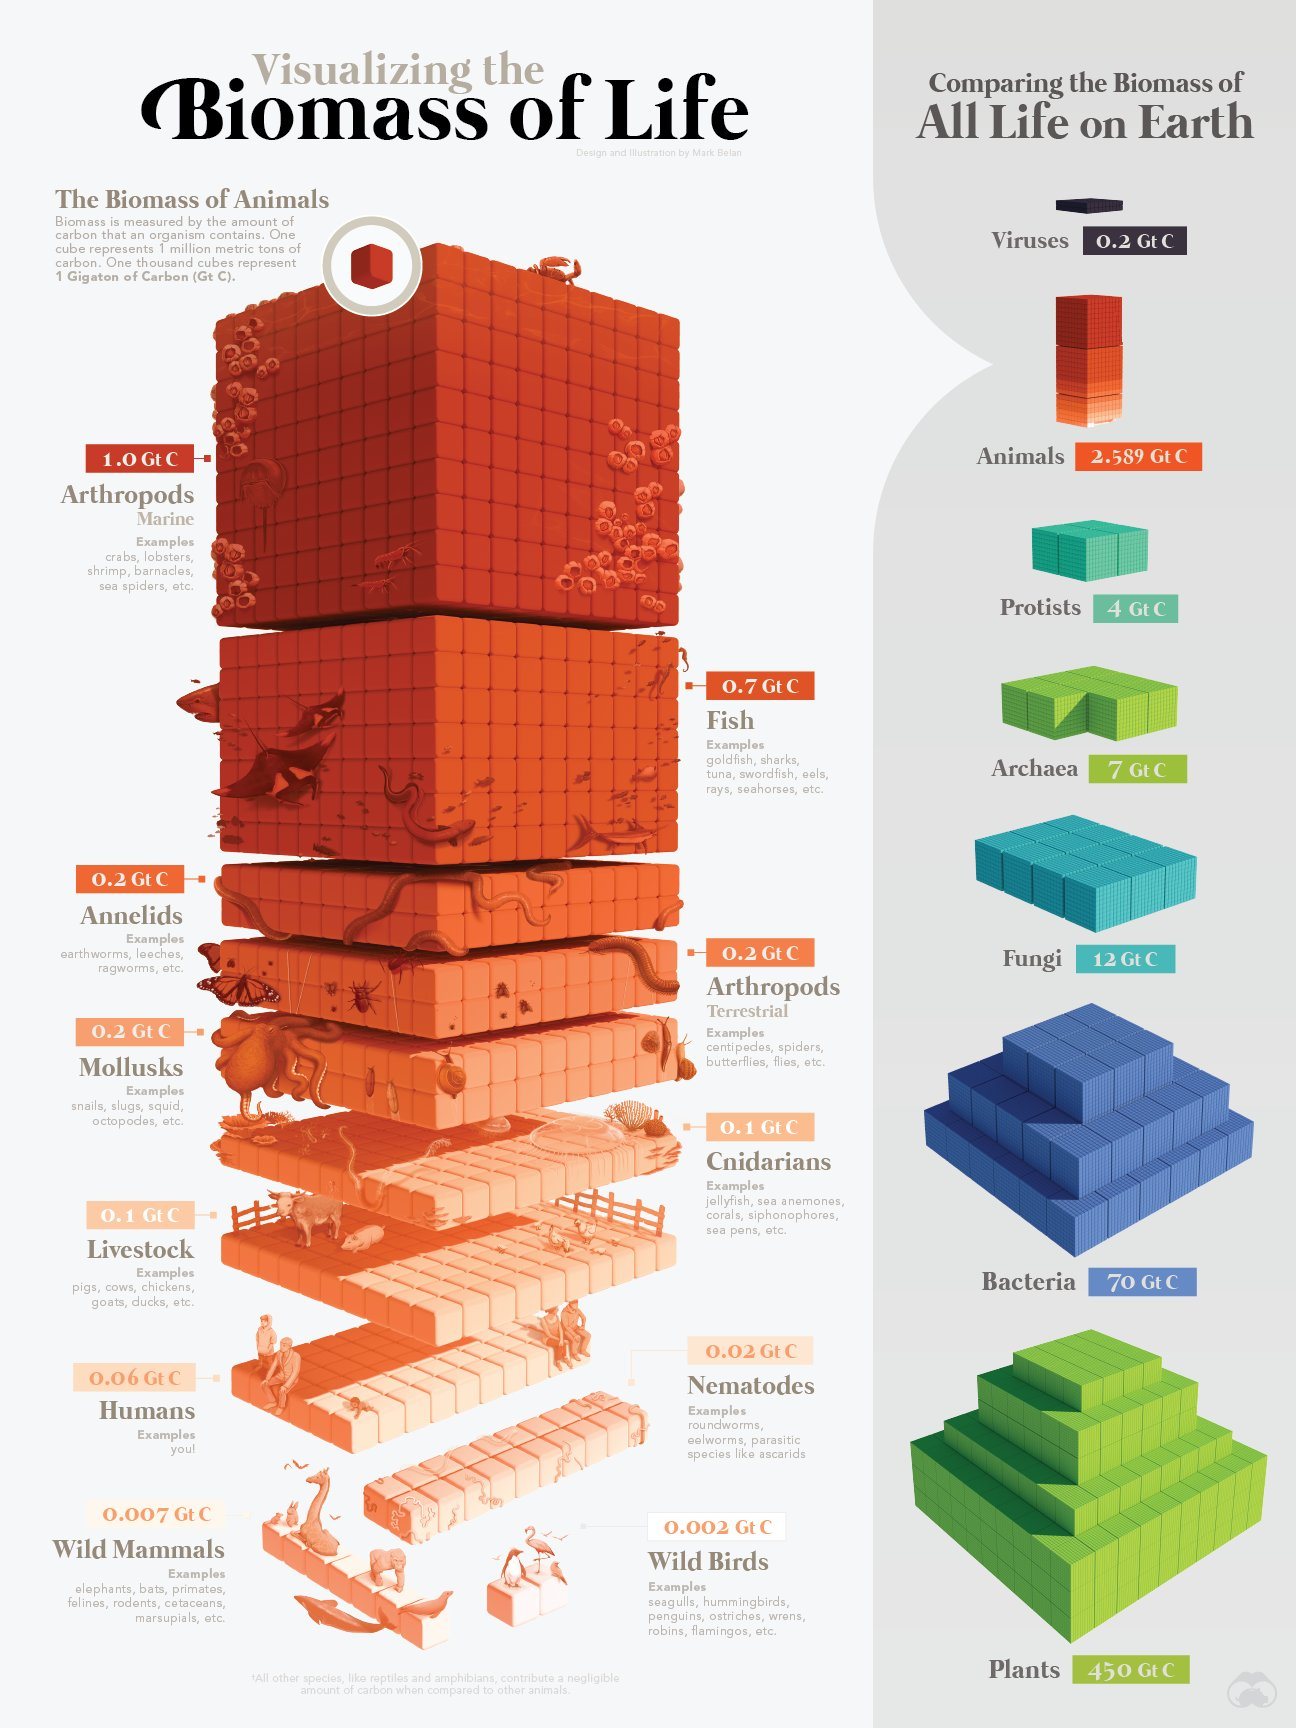
\includegraphics[width=0.8\linewidth]{../images/biomass_of_life}

\ecolumns
\end{frame}

\begin{frame}{Distinction of stages of variation in plants and
pathogens}
\protect\hypertarget{distinction-of-stages-of-variation-in-plants-and-pathogens}{}
Refer to Page 134, \citet{agrios2005plant}.
\end{frame}

\begin{frame}{Identification of physiological races and pathotypes}
\protect\hypertarget{identification-of-physiological-races-and-pathotypes}{}
\footnotesize

\begin{itemize}
\tightlist
\item
  Concepts of physiological races was introduced by Barrus in 1911.
\item
  To identify and distinguish different species of a pathogen and
  races/strains within a species `differential hosts' are used.

  \begin{description}
  \small
  \item[Differential host] are the varieties of host species used to identify physiological races of a pathogen or sets of plant cultivars used to define pathotypes of pathogen based on known susceptible and resistant reactions
  \end{description}
\item
  Maximum number of races identifiable with \(n\) number of differential
  hosts is given by relation,
\end{itemize}

\[
\small
\text{Number of races identifiable} = r^n
\] - Where,

\begin{itemize}
  \item $r$ = number of reaction types identifiable (e.g. resistant or susceptible, or others.)
  \end{itemize}

\begin{itemize}
\tightlist
\item
  If only two types of host-pathogen reaction are recorded
  (i.e.~resistant and susceptible), a set of \(n\) ideal differentials
  would identify \(2^n\) physiological races.
\item
  Ideally, each of the differential hosts should posses a single
  resistance gene different from those present in the others.
\end{itemize}
\end{frame}

\begin{frame}{}
\protect\hypertarget{section-1}{}
\ldots{}
\end{frame}

\begin{frame}{Insects and Diseases of Major Crops in Nepal}
\protect\hypertarget{insects-and-diseases-of-major-crops-in-nepal}{}
\begin{table}[H]

\caption{\label{tab:insect-pests-major}Major disease and insect pests of major cultivated crops in Nepal}
\centering
\fontsize{6}{8}\selectfont
\begin{tabular}[t]{l>{\raggedright\arraybackslash}p{20em}>{\raggedright\arraybackslash}p{20em}}
\toprule
Crop & Major insects & Major disease\\
\midrule
\cellcolor{gray!6}{Rice} & \cellcolor{gray!6}{Rice bug, rice hispa, yellow stem borer, stripped stem borer, rice gall midge, mole cricket, plant hopper} & \cellcolor{gray!6}{Bacterial blight (Xanthomonas oryzae), Blast (Pyricularia oryzae), False smut (Ustilaginoides virens), Brown leaf spot (Helminthosporium oryzae)}\\
Wheat & Armyworm, cutworm, shoot fly, stem borer, termites & Leaf spots (Helminthosporium spp), rust, leaf streak (Xanthomonas spp), loose smut\\
\cellcolor{gray!6}{Maize} & \cellcolor{gray!6}{Stalk borer, shoot fly, cutworm, jassid, armyworm} & \cellcolor{gray!6}{Rust, leaf blight (Helminthosporium maydis), smut (Specealothica reliana)}\\
Barley & Green bug, corn sawfly, fruitfly, wheat bulb fly & Barley yellow dwarf virus, powdery mildew (Erysiphe graminis sp. hordii), Net blotch (Helminthosporium sativum)\\
\bottomrule
\end{tabular}
\end{table}
\end{frame}

\hypertarget{diseases}{%
\section{Diseases}\label{diseases}}

\begin{frame}{}
\protect\hypertarget{section-2}{}
\begin{table}

\caption{\label{tab:fungal-pseudo-fungal-classification}Classification of fungi and fungal-like organisms that cause disease on plants.}
\centering
\fontsize{4}{6}\selectfont
\begin{tabular}[t]{>{\raggedright\arraybackslash}p{10em}>{\raggedright\arraybackslash}p{18em}>{\raggedright\arraybackslash}p{16em}>{\raggedright\arraybackslash}p{12em}>{\raggedright\arraybackslash}p{28em}}
\toprule
Group & Phylum (Super/Phy/Sub/Infra) & Class & Order & Features\\
\midrule
 &  &  &  & Produce a plasmodium or plasmodium like structure\\
\cmidrule{3-5}
 &  & Dictyosteliida &  & Cellular slime molds\\
\cmidrule{3-5}
\multirow{-3}{*}{\raggedright\arraybackslash Domain: Eukaryota} & \multirow{-3}{*}{\raggedright\arraybackslash Phylum: Amebozoa, Infra-phylum: Mycetozoa} & Myxogastria &  & Plasmodial slime molds\\
\cmidrule{1-5}
 & Phylum: Cercozoa (as Rhizaria is a part of SAR assemblages (Stramenopiles+Alveolates+Rhizaria), shares common ancestory with Stramenopiles) & Phytomyxea & Plasmodiophorida & Endoparasitic slime molds\\
\cmidrule{2-5}
\multirow{-2}{*}{\raggedright\arraybackslash Kingdom: Chromista} & Super-phylum: Heterokonta/Stramenopiles, Subphylum: Pseudofungi & Oomycetes & Peronosporales (Families: Albuginaceae, Peronosporaceae, Pythiaceae) (eg) & Stramenopiles have two different flagella, one having hollow tripartite hairs; Peronosporales have elongated non-septate mycelium, biflagellate zoospores in zoosporangia, oospores\\
\cmidrule{1-5}
 &  & Division: Chytridiomycota, Class: Chytridiomycetes & Chytridiales (eg) & Have zoospores with a single posterior flagellum, round or elongated mycelium\\
\cmidrule{3-5}
 &  & Division: Zygomycota &  & Produce non-motile asexual spores in sporangia. Resting spore is a zygospore\\
\cmidrule{3-5}
 &  & Division: Ascomycota &  & Produce sexual spores, ascospores, in asci. Produce nonmotile asexual spores (conidia)\\
\cmidrule{3-5}
\multirow{-4}{*}{\raggedright\arraybackslash Kingdom: Fungi} & \multirow{-4}{*}{\raggedright\arraybackslash Eumycota} & Division: Basidiomycota &  & Produce sexual spores, basidiospores, externally on a basidium\\
\bottomrule
\end{tabular}
\end{table}

(\scriptsize For a more descriptive classification refer to
\citet{agrios2005plant}, section on Classification of plant pathogenic
fungi, Chapter 11 -- Plant diseases caused by fungi.)
\end{frame}

\begin{frame}{}
\protect\hypertarget{section-3}{}
\begin{center}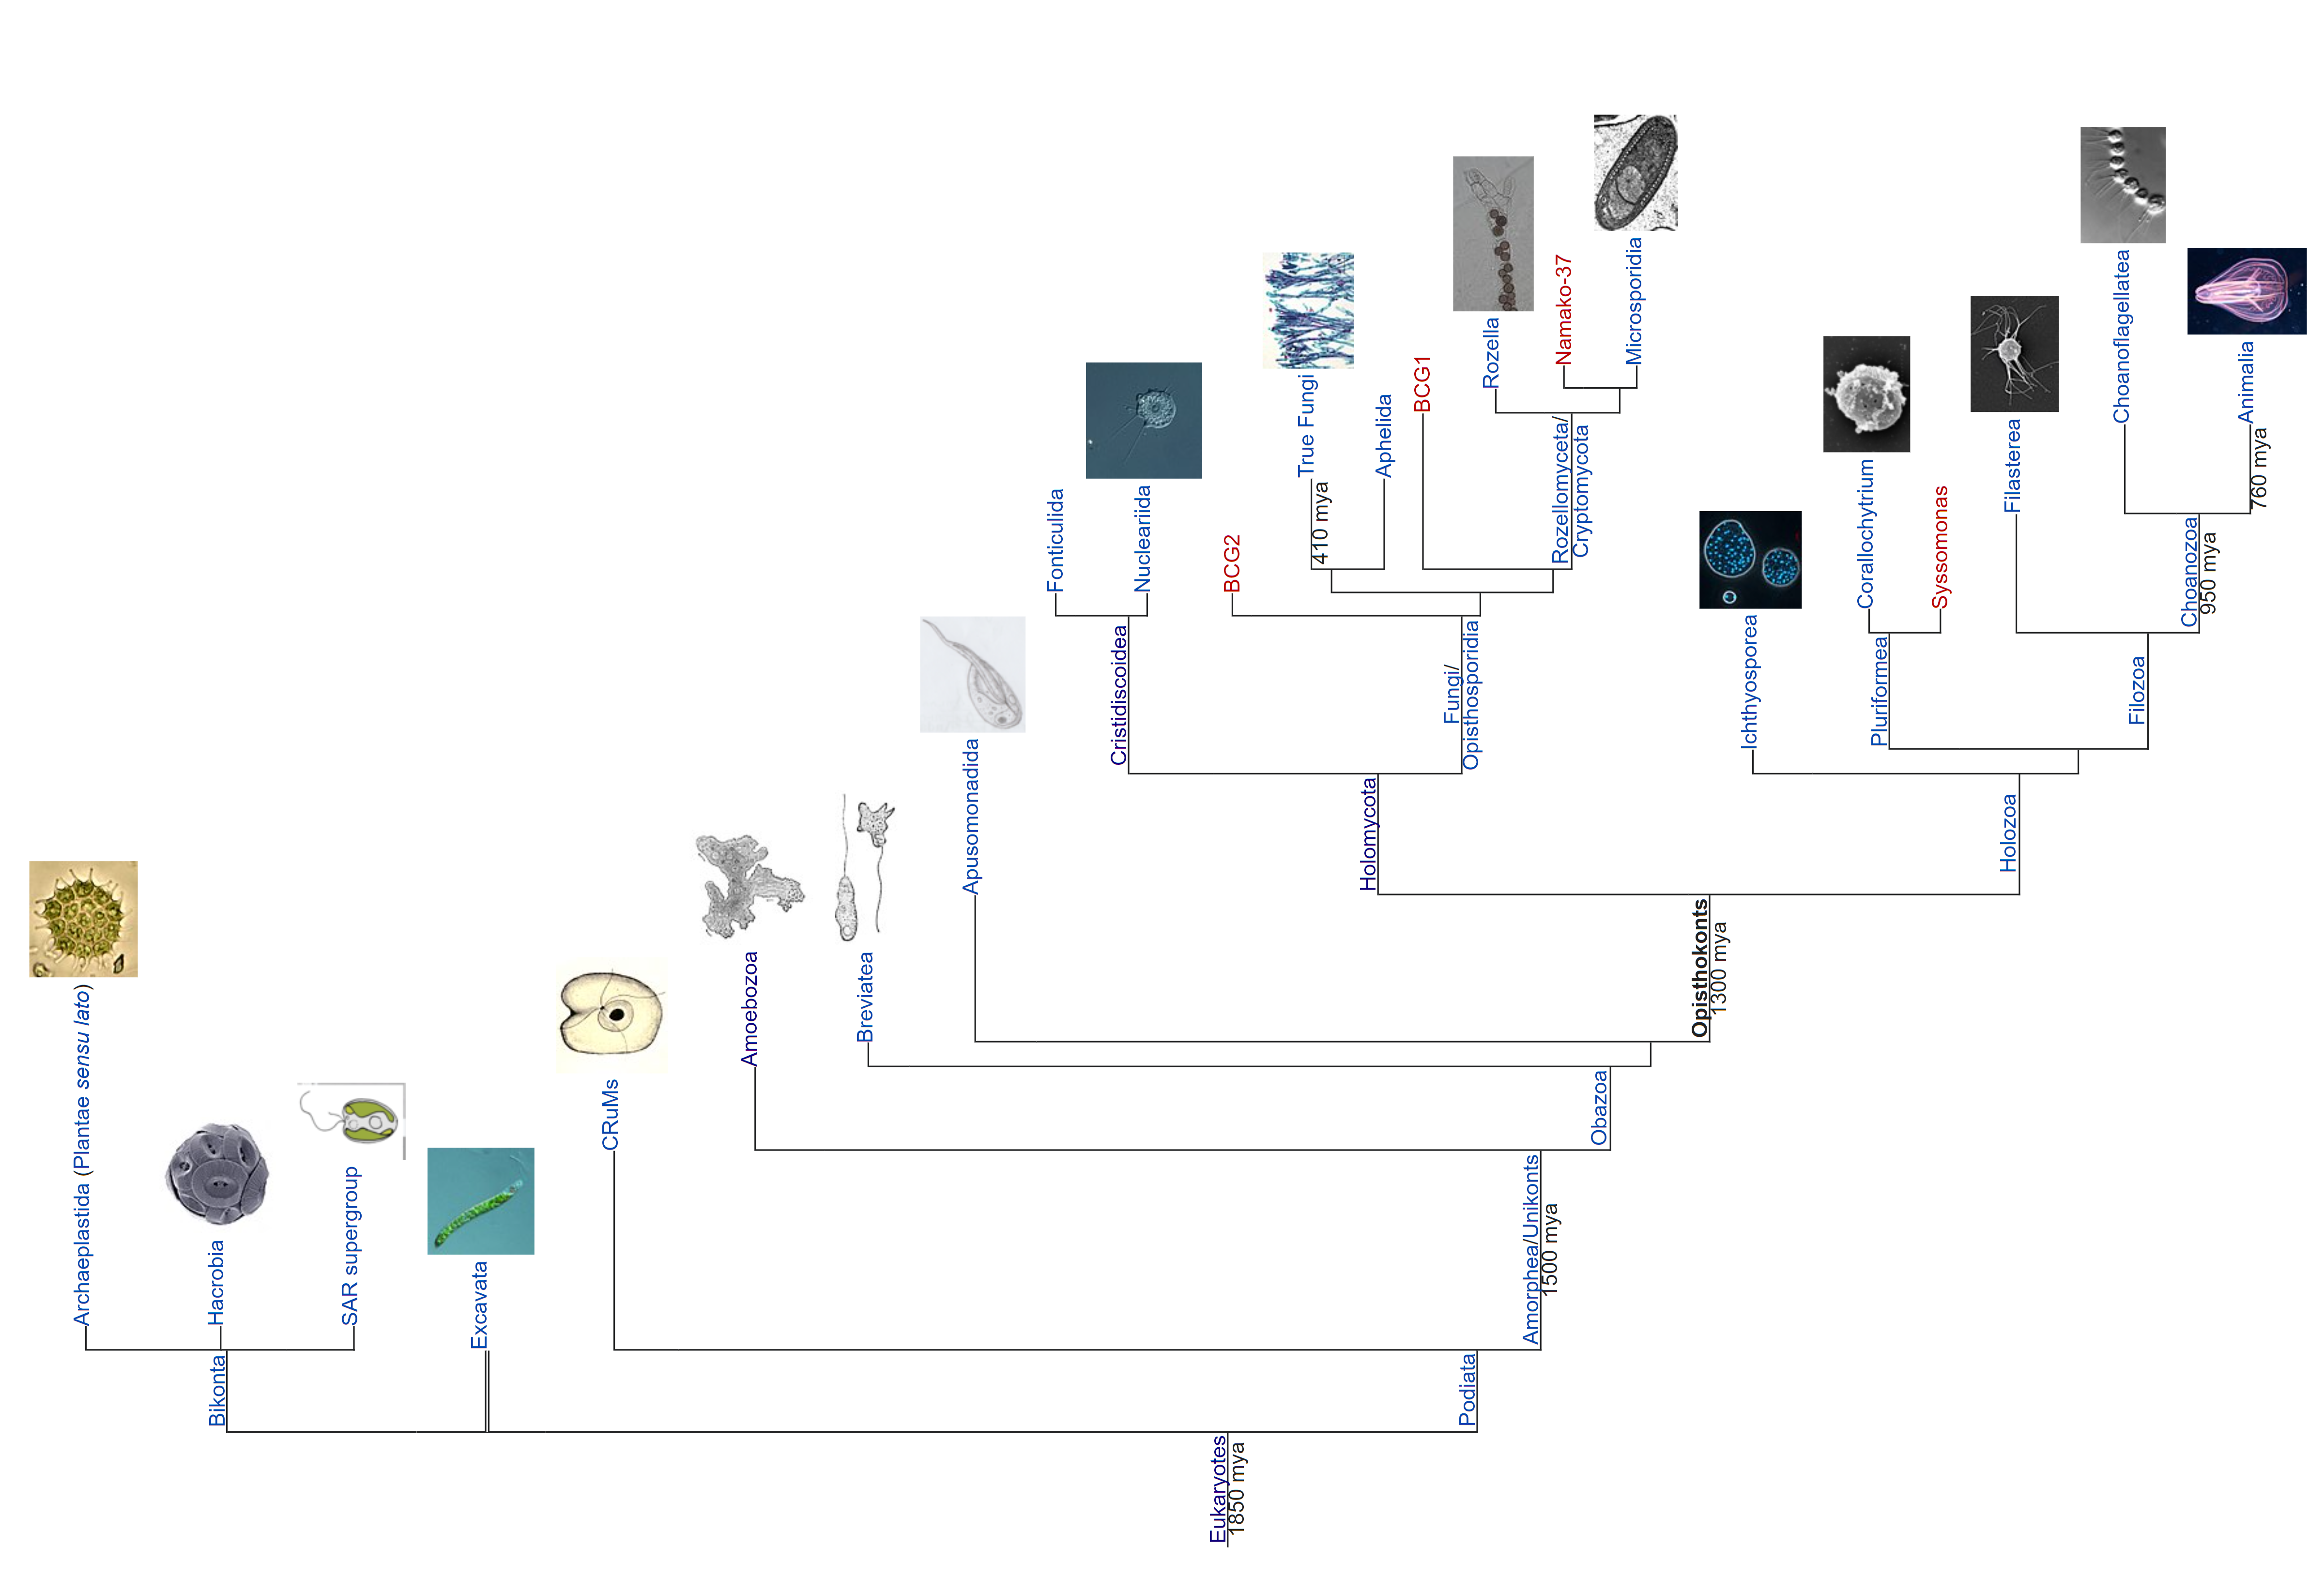
\includegraphics[width=0.84\linewidth]{../images/wiki_opisthokonta} \end{center}
\end{frame}

\begin{frame}{}
\protect\hypertarget{section-4}{}
\bcolumns
\column{0.6\textwidth}

\begin{figure}
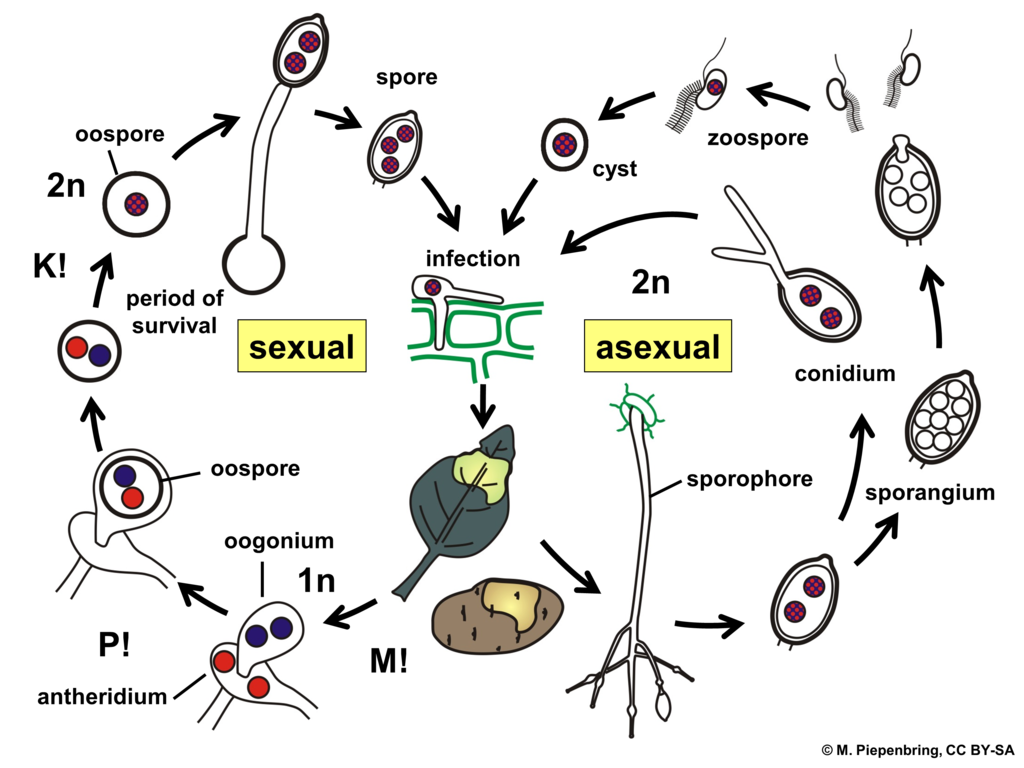
\includegraphics[width=0.9\linewidth]{../images/Phytophthora_infestans_on_potato} \caption{Life cycle of phytophthora infestans}\label{fig:phytophthora-infestans-life-cycle}
\end{figure}

\column{0.4\textwidth}

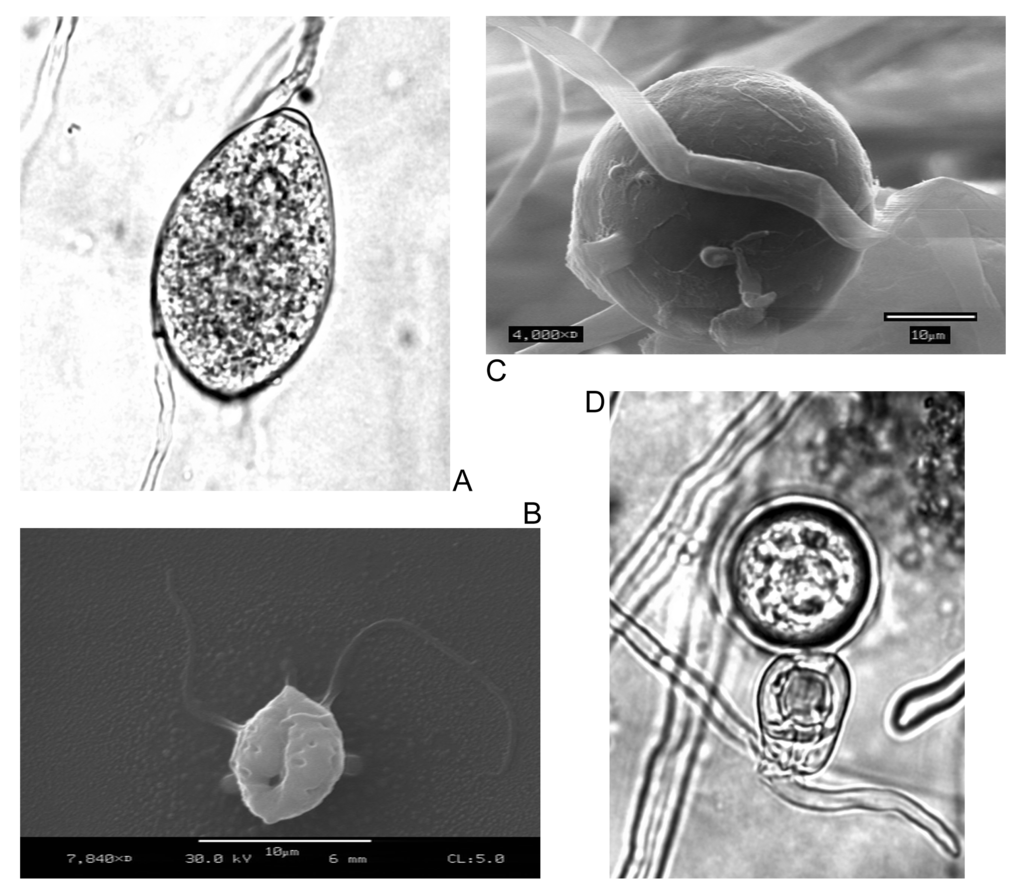
\includegraphics[width=0.8\linewidth]{../images/Phytophtora_reproduction}

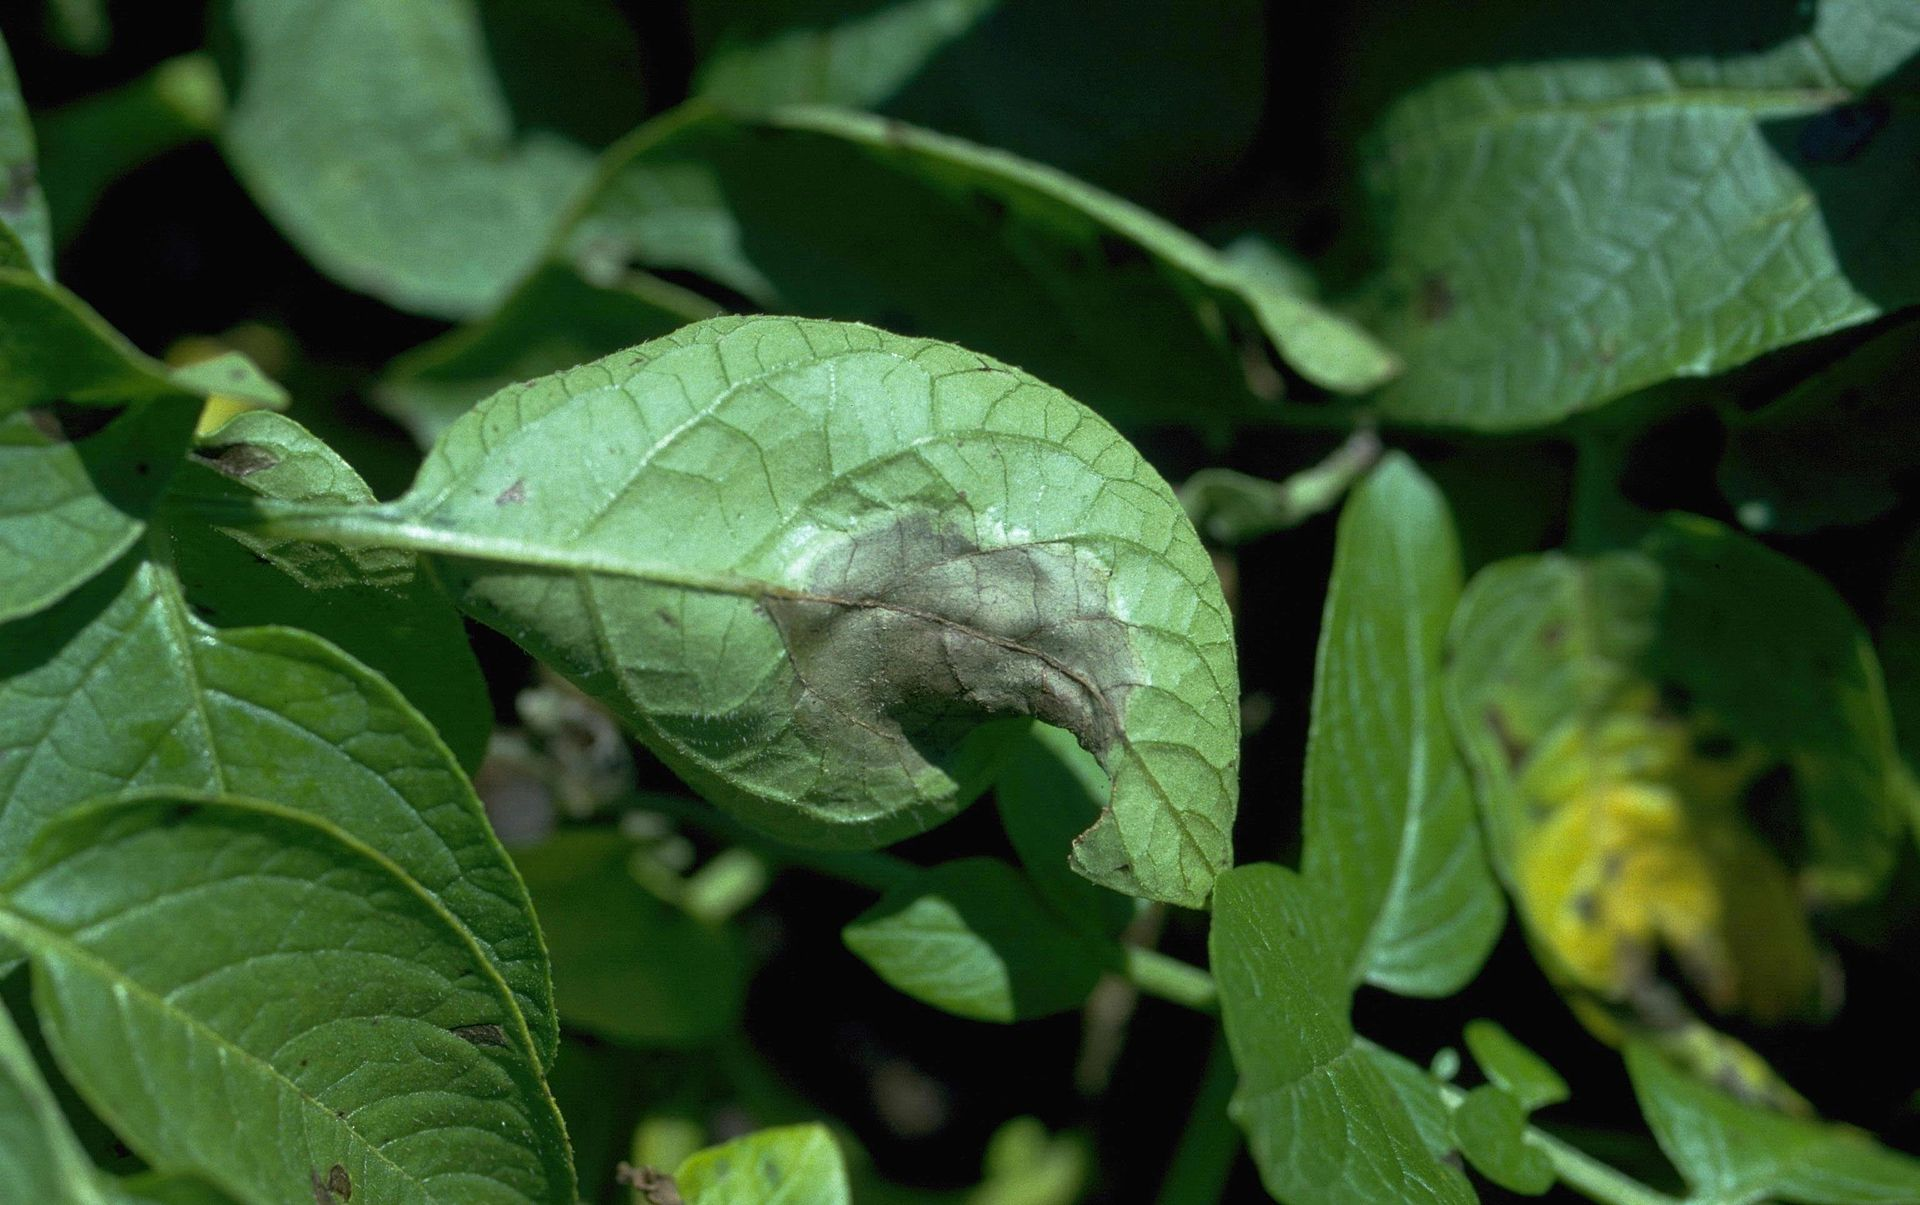
\includegraphics[width=0.8\linewidth]{../images/Late_blight_on_potato_leaf}

\ecolumns
\end{frame}

\begin{frame}{}
\protect\hypertarget{section-5}{}
\begin{itemize}
\tightlist
\item
  Most pathogenic fungi belong to phyla Ascomycota and Basidiomycota
\item
  Fungi reproduce both sexually and asexually via the production of
  spores and other structures
\item
  Basidiomycetes

  \begin{itemize}
  \tightlist
  \item
    produce sexual spores called basidiospores, on a club-shaped
    spore-producing structure called a basidium
  \item
    mostly are fleshy fungi such as common mushrooms, the puffballs, and
    the shelf fungi or conks, and are either saprophytes or cause wood
    decay, including root and stem rots of trees.
  \item
    two most destructive groups of plant pathogenic fungi -- rust
    (Pucciniomycotina) and smut (Ustilaginomycotina) -- are contained
  \item
    characterized by basidia as meiosporocysts in the sexual life stage
  \item
    karyogamy and meiosis proceed in the basidia and basidiospores are
    produced
  \item
    basidiomycetous hyphae, which have an electron-dense (multi-layered
    or visually single-layered) wall, are divided by septa into
    mononucleate, binucleate, or multinucleate segments
  \item
    according to Ainsworth and Bisby's Dictionary of Fungi (2008), there
    are 1589 genera and more than 30,000 species of Basidiomycoa (32\%
    of all described fungal taxa)
  \end{itemize}
\end{itemize}
\end{frame}

\begin{frame}{}
\protect\hypertarget{section-6}{}
\begin{itemize}
\tightlist
\item
  Ascomycota

  \begin{itemize}
  \footnotesize
  \item 98\% of lichens have an Ascomycota as the fungal part (symbiotic association) of the lichen.
  \item 2000 identified genera and 30,000 species of Ascomycota. Most ascomycetes are terrestrial or parasitic. However, some have adapted to marine or freshwater environments.
  \item Presence of a reproductive structure known as the ascus, though in some cases it has a reduced role in the life cycle.
  \item Used as yeasts in baking/brewing and treated as delicacies as truffles and morels. The mold Penicillium is used to produce the antibiotic penicillin.
  \item Many cause tree diseases, such as Dutch elm disease and apple blights. Some of the plant pathogenic ascomycetes are apple scab, rice blast, the ergot fungi, black knot, and the powdery mildews.
  \item Morels (a highly prized edible fungi) form important mycorrhizal relationships with plants, thereby providing enhanced water and nutrient uptake and, in some cases, protection from insects.
  \item The cell walls of the hyphae are variably composed of chitin and $\beta$-glucans, just as in Basidiomycota. However, these fibers are set in a matrix of glycoprotein containing the sugars galactose and mannose.
  \item The mycelium of ascomycetes is usually made up of septate hyphae. However, there is not necessarily any fixed number of nuclei in each of the divisions.
  \item The septal walls have septal pores which provide cytoplasmic continuity throughout the individual hyphae. Under appropriate conditions, nuclei may also migrate between septal compartments through the septal pores.
  \item A unique character (but not present in all ascomycetes) is the presence of Woronin bodies on each side of the septa separating the hyphal segments which control the septal pores.
  \end{itemize}
\end{itemize}
\end{frame}

\begin{frame}{}
\protect\hypertarget{section-7}{}
\begin{figure}
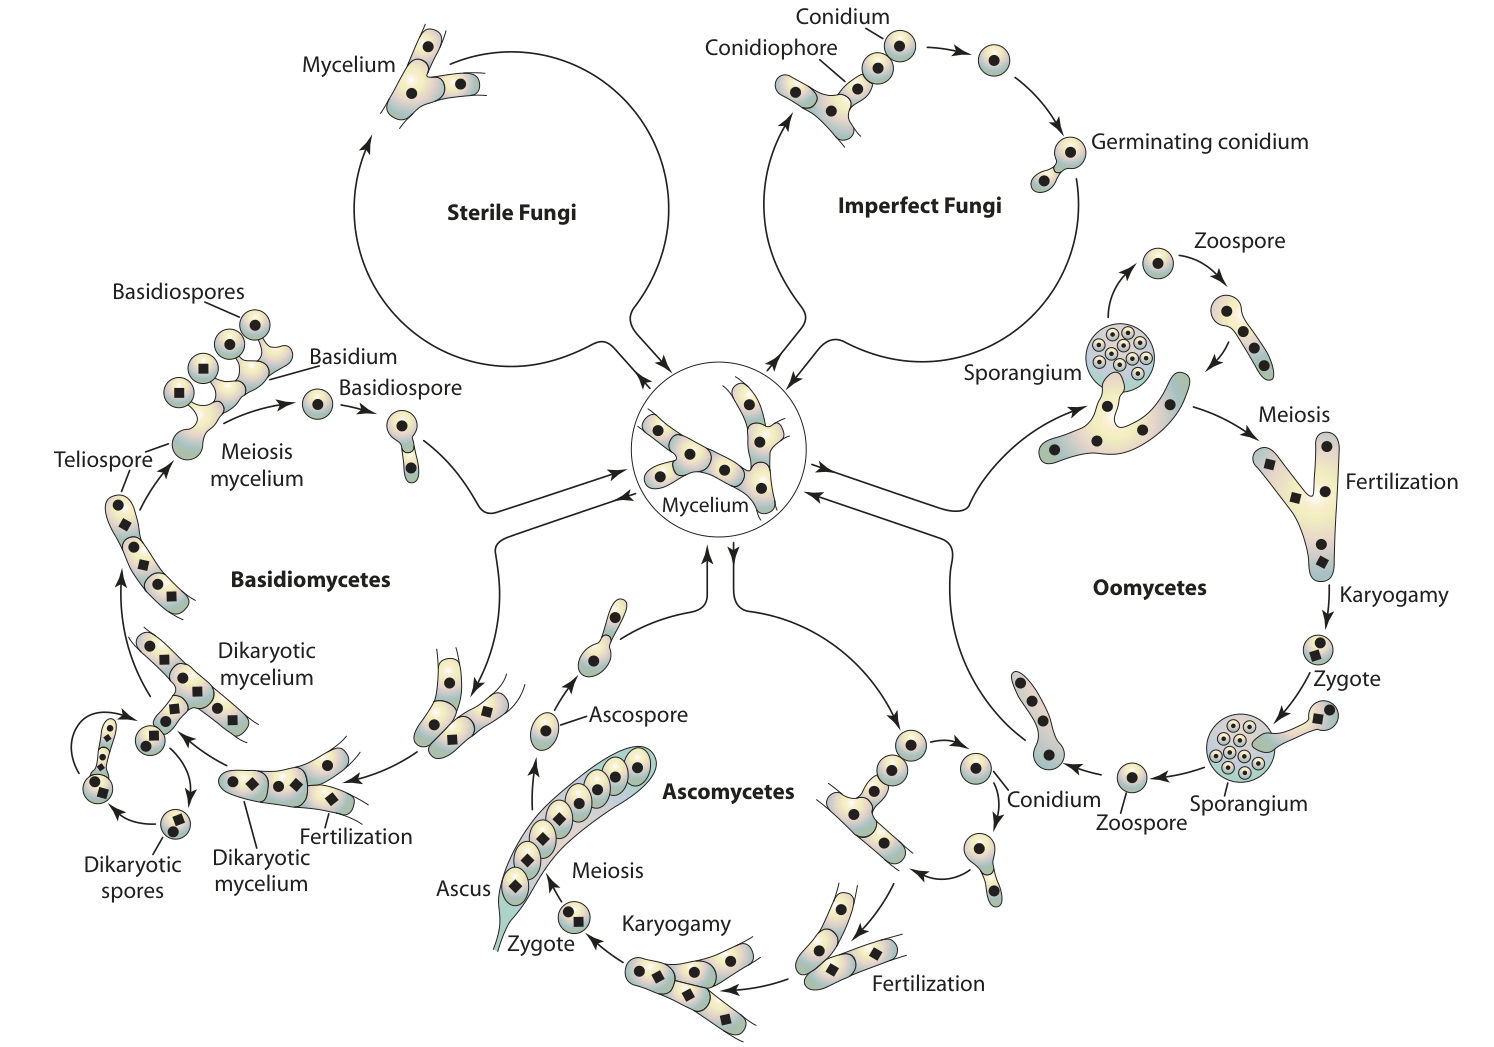
\includegraphics[width=0.72\linewidth]{../images/generalized_life_cycle_pathogenic_fungi} \caption{Schematic representation of the genralized life cycles of oomycetes and the main groups of phytopathogenic fungi.}\label{fig:life-cycle-plant-pathogenic-fungi}
\end{figure}
\end{frame}

\begin{frame}{Rust and smut}
\protect\hypertarget{rust-and-smut}{}
\begin{itemize}
\tightlist
\item
  Rust fungi are obligate parasites in nature
\item
  Notorious on grain crops (wheat, oats, barley), vegetables (bean,
  asparagus), field crops (cotton, soybeans), ornamentals (carnation,
  chrysanthemum, snapdragon) and trees (pine, apple, coffee)
\item
  Infection usually appear numerous rusty, orange, yellow, or even
  white-colored spots that rupture the epidermis. Some form swellings
  and even galls. Most rust infections are strictly local spots, but
  some may become systemic.
\item
  There are about 5000 species of rust fungi.
\item
  Sexual reproduction tends to promote rapid development of new races.
\item
  Rust caused by fungi that produce only teliospores and basidiospores
  are called microcyclic or short cycled.
\end{itemize}
\end{frame}

\begin{frame}{Common rust fungi in agriculture}
\protect\hypertarget{common-rust-fungi-in-agriculture}{}
\begin{itemize}
\tightlist
\item
  \emph{Hemileia vastatrix} (Coffee rust); Primary host is coffee plant;
  unknown alternate host. Heteroecious
\item
  \emph{Phakopsora meibomiae} and \emph{P. pachyrhizi} (Soybean rust);
  Primary host is soybean and various legumes. Unknown alternate host.
  Heteroecious
\item
  \emph{Puccinia coronata} (Crown Rust of Oats and Ryegrass); Oats are
  the primary host; Rhamnus spp. (Buckthorn) is alternate host.
  Heteroecious and macrocyclic
\item
  \emph{Puccinia graminis} (Stem rust of wheat and Kentucky bluegrass,
  or black rust of cereals); Primary hosts include: Kentucky bluegrass,
  barley, and wheat; Common barberry is the alternate host. Heteroecious
  and macrocyclic
\item
  \emph{Puccinia hemerocallidis} (Daylily rust); Daylily is primary
  host; Patrina sp is alternate host. Heteroecious and macrocyclic
\item
  \emph{Puccinia triticina} (Brown Wheat Rust) in grains
\item
  \emph{Puccinia sorghi} (Common Rust of Corn)
\item
  \emph{Puccinia striiformis} (Yellow Rust) of cereals
\item
  \emph{Uromyces appendiculatus} (Bean Rust) in common bean (Phaseolus
  vulgaris)
\item
  \emph{Puccinia melanocephala} (Brown Rust of Sugarcane)
\item
  \emph{Puccinia kuehnii} (Orange rust of Sugarcane)
\end{itemize}
\end{frame}

\begin{frame}{}
\protect\hypertarget{section-8}{}
\begin{itemize}
\tightlist
\item
  \emph{Puccinia graminis} is a macrocyclic (produces one or more of
  spermatia, aeciospores and uredospores) heteroecious fungus that
  causes wheat stem rust disease.
\item
  The repeating stage (allows the disease to persist) in this fungus
  occurs on wheat and not the alternate host, barberry.
\end{itemize}

\begin{columns}[T, onlytextwidth]
\column{0.5\textwidth}

\begin{figure}
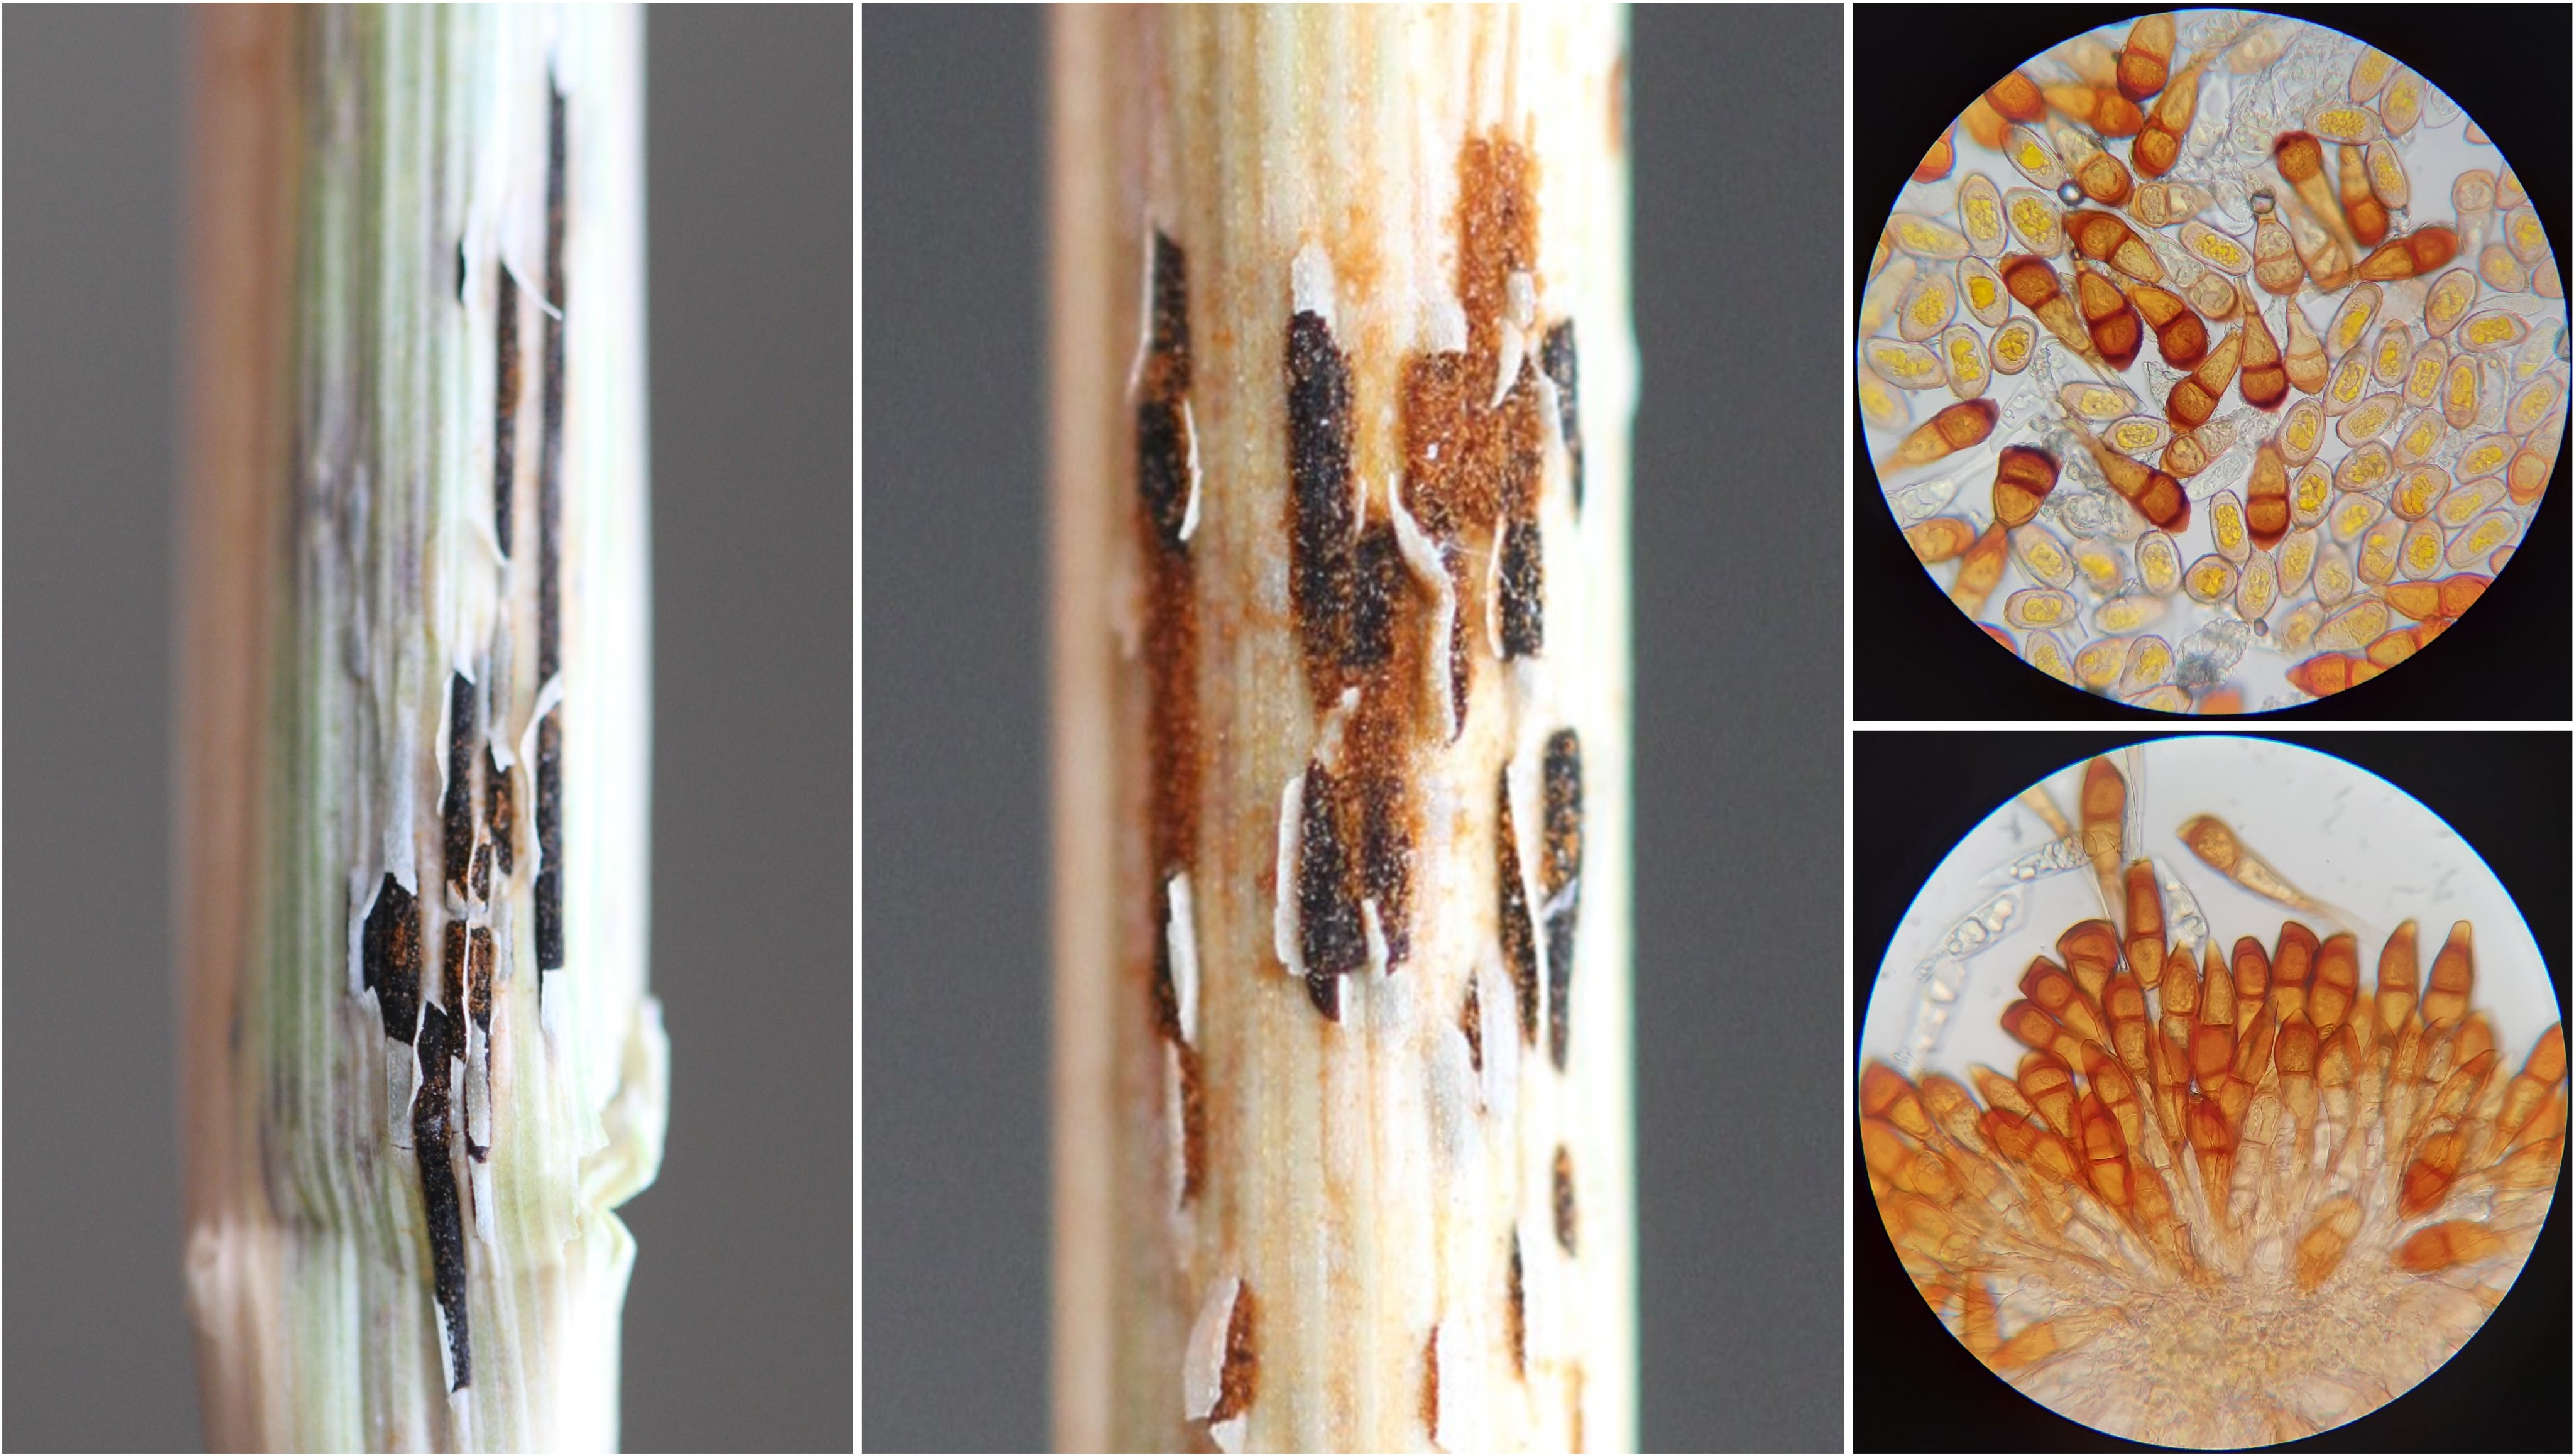
\includegraphics[width=0.8\linewidth]{../images/stem_rust_wheat_puccinia_graminis_f.sp.tritici} \caption{Stem rust of Wheat (\textit{Triticum aestivium}) caused by \textit{Puccinia graminis} f. sp. tritici, here with urediniospores and teliospores (First pic shows telia and the second a mix of telia and uredinia).}\label{fig:puccinia-graminis-wheat}
\end{figure}

\column{0.5\textwidth}

\begin{figure}
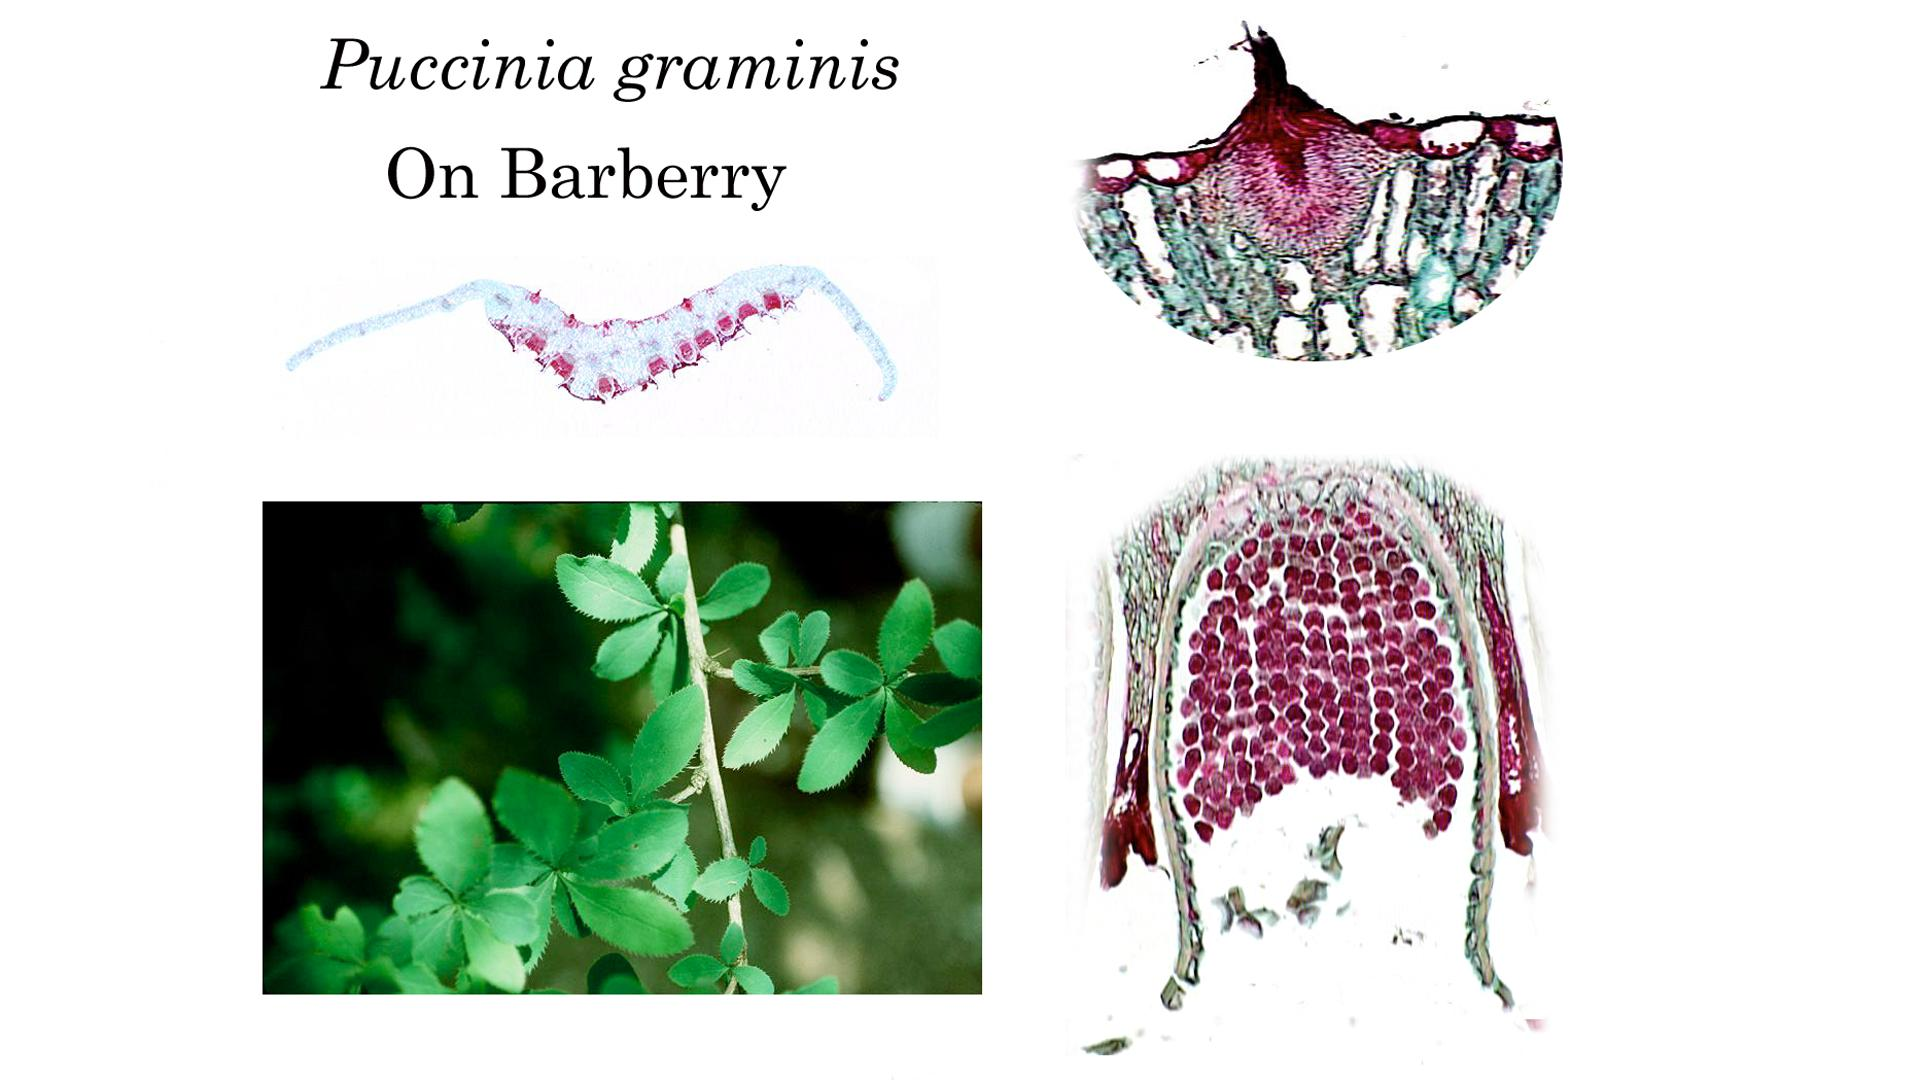
\includegraphics[width=0.85\linewidth]{../images/berberry_aecium} \caption{Wheat rust infection on barberry; Cross section of infected leaf, spermagonium on upper leaf, leafy bough of barberry, aecium with aeciospores on lower leaf surface. These spores are dikaryotic (they each have two haploid nuclei of different genetic make-up). These go on to infect wheat. The aeciospores are borne in chains and are held together by little rectangular cells called disjunctors.}\label{fig:berberry-aecium}
\end{figure}

\end{columns}
\end{frame}

\begin{frame}{}
\protect\hypertarget{section-9}{}
\begin{itemize}
\tightlist
\item
  Because there is no repeating stage in the life cycle of demicyclic
  fungi, removal of the primary or the alternate host will disrupt the
  disease cycle.
\item
  Cedar-apple rust disease, for example, can persist despite removal of
  one of the hosts since spores can be disseminated from long distances

  \begin{itemize}
  \tightlist
  \item
    severity of this disease can be managed by removal of basidiospore
    producing galls from junipers or the application of protective
    fungicides to junipers.
  \end{itemize}
\item
  Sulphur powder is known to stop spore germination. Fungicides such as
  Mancozeb and Triforine may help but may never eradicate the disease.
\end{itemize}
\end{frame}

\begin{frame}{UG99}
\protect\hypertarget{ug99}{}
\begin{columns}[T, onlytextwidth]
\column{0.6\textwidth}

It is a lineage of wheat stem rust ( \textit{Puccinia graminis} f. sp. \textit{tritici}), which is present in wheat fields in several countries in Africa and Middle east and is predicted to spread rapidly through these regions and possibly further afield, potentially causing a wheat production disaster that would affect food security worldwide. It can cause up to 100% crop losses and is virulent against many resistance genes which have previously protected against stem rust.

\column{0.4\textwidth}

\begin{figure}
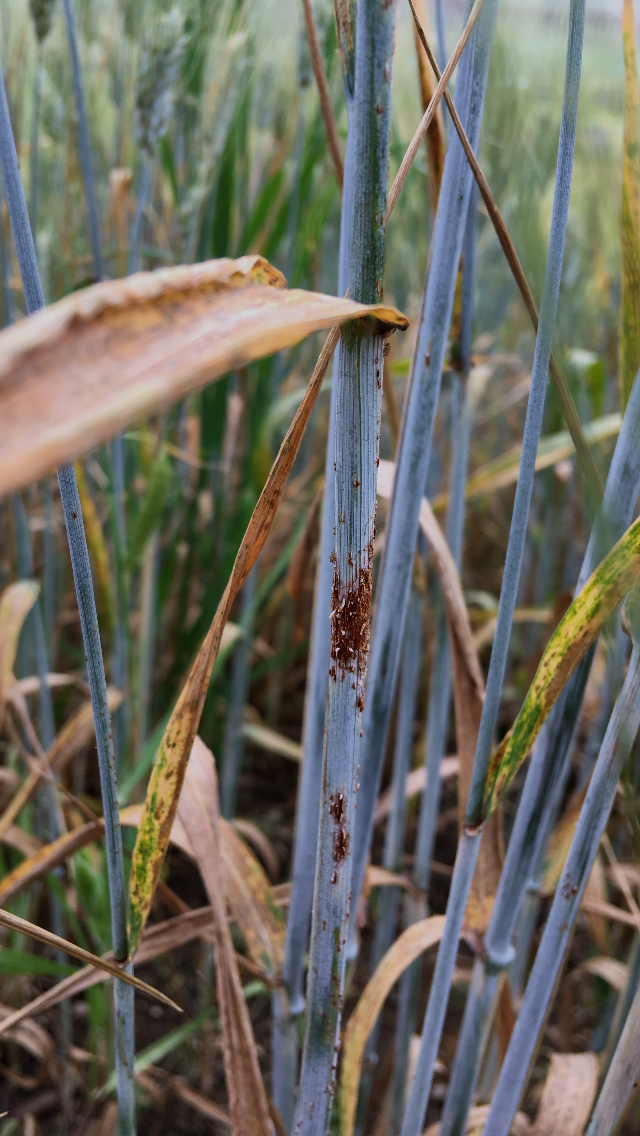
\includegraphics[width=0.6\linewidth]{../images/B5_StemRust} \caption{Stem rust (race B5) on Wheat.}\label{fig:stem-rust}
\end{figure}

\end{columns}
\end{frame}

\begin{frame}{}
\protect\hypertarget{section-10}{}
\begin{columns}[T, onlytextwidth]
\column{0.4\textwidth}

\begin{figure}
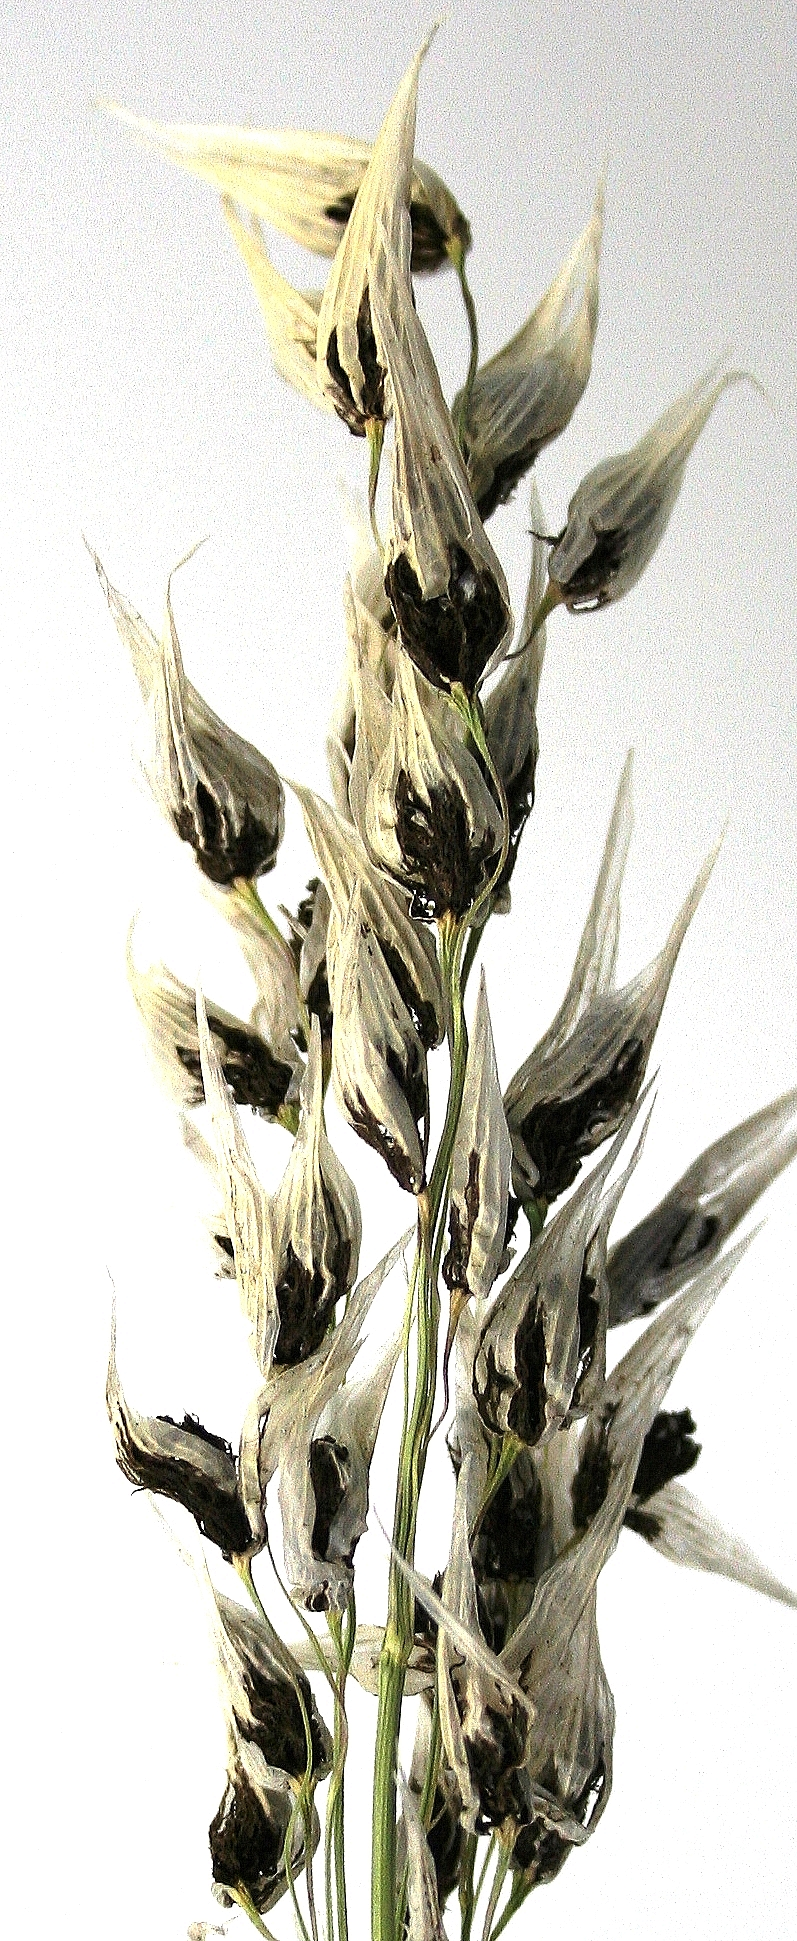
\includegraphics[width=0.45\linewidth]{../images/ustilago_avenae} \caption{Smut head of Oat caused by \textit{Ustilago avenae}.}\label{fig:avenae-smut}
\end{figure}

\column{0.6\textwidth}

\begin{figure}
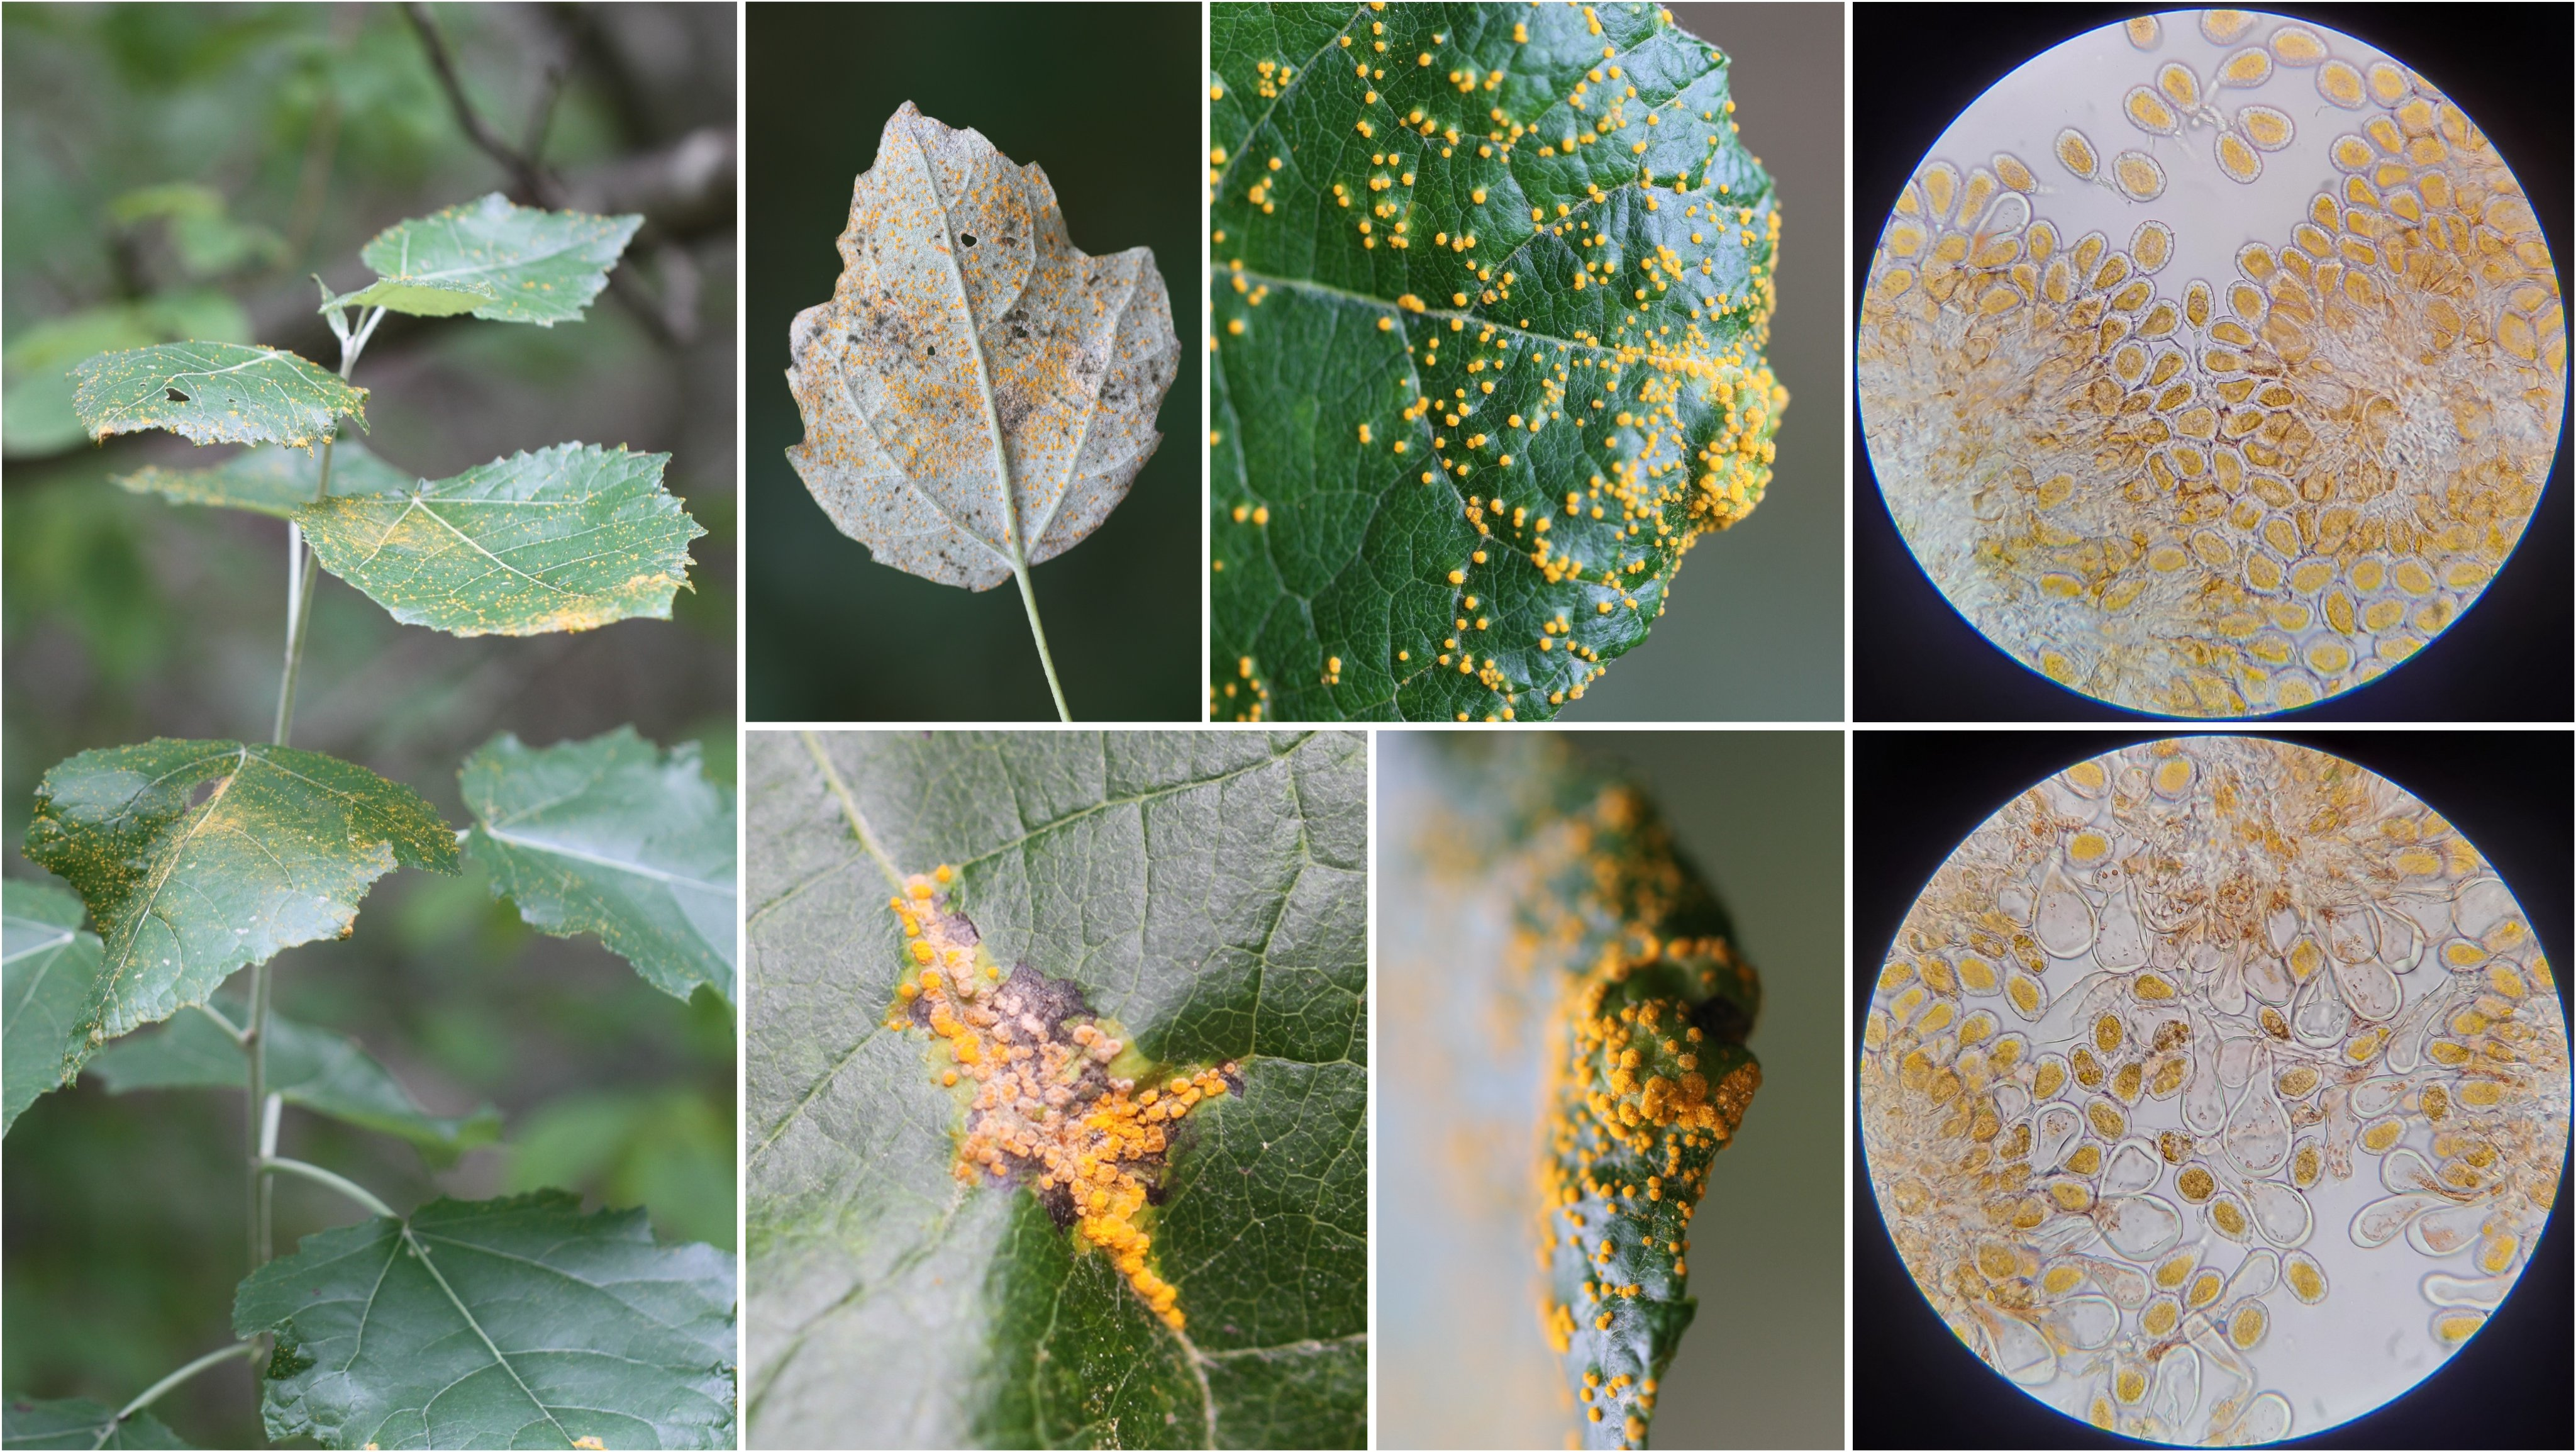
\includegraphics[width=0.95\linewidth]{../images/FdhD0Z3XoAIf1OB} \caption{Rust on White poplar \textit{Populus alba} caused by \textit{Melampsora} sp.. Uredinia are protruding on the upper face of some leaves and in cluster on ribs.}\label{fig:poplar-rust}
\end{figure}

\end{columns}
\end{frame}

\begin{frame}{}
\protect\hypertarget{section-11}{}
\begin{figure}\caption{Stem rust on UK breeding nurseries}\begin{columns}\column{0.5\textwidth}

\begin{center}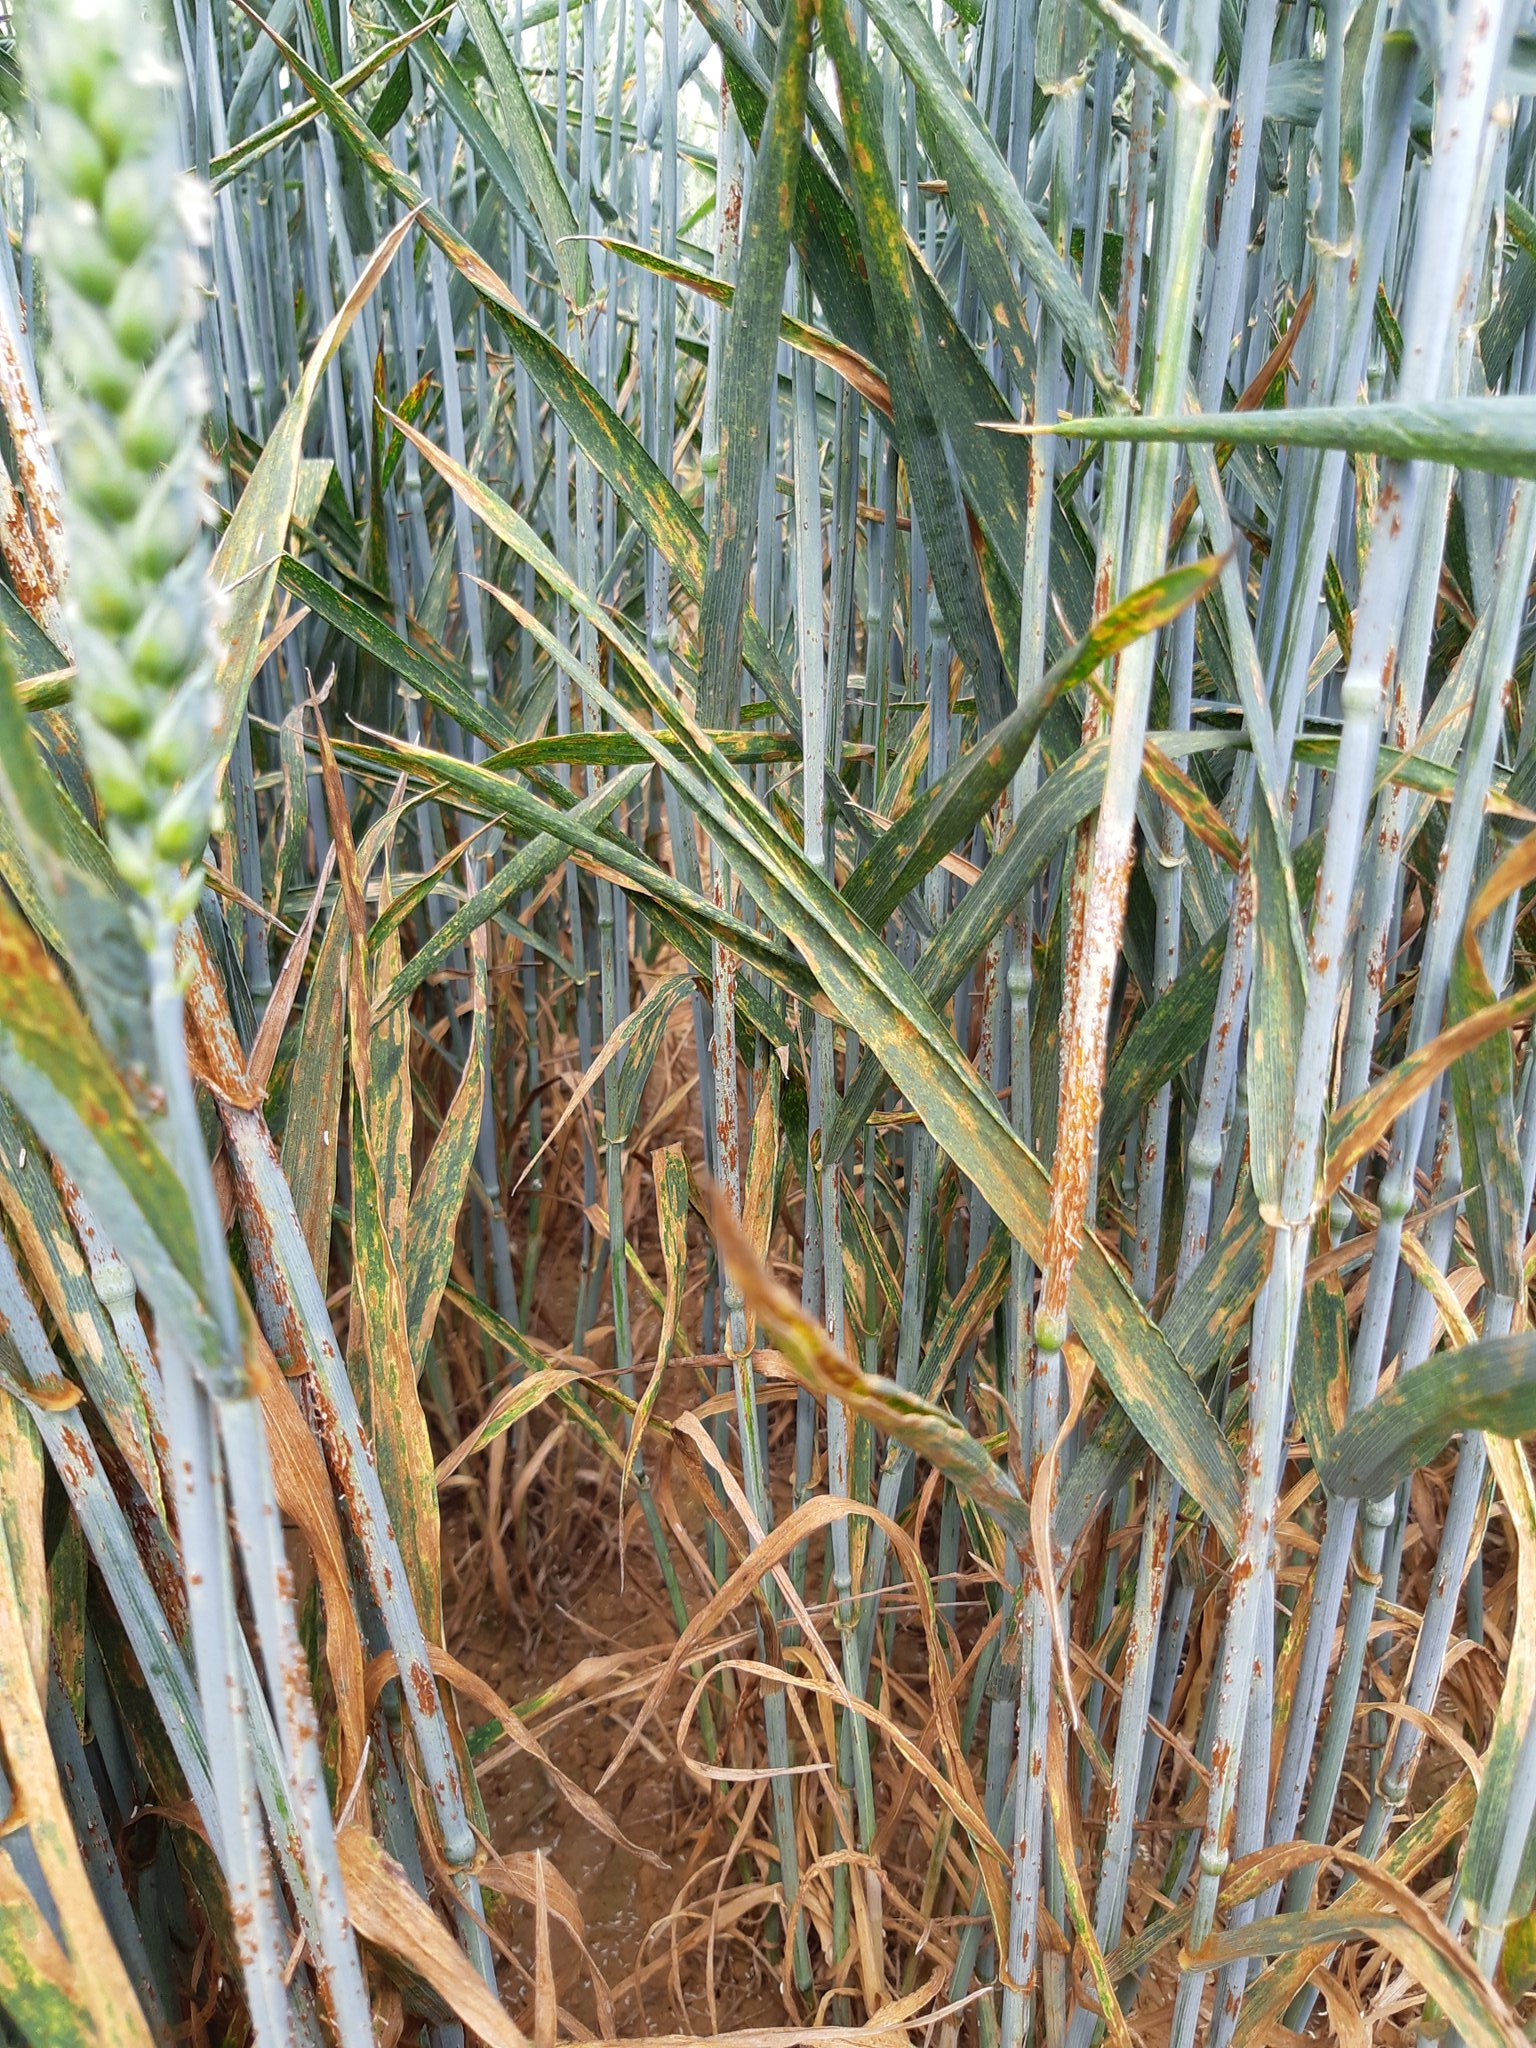
\includegraphics[width=0.55\linewidth]{../images/FWGDjevXwAEBzeT} \end{center}

\column{0.5\textwidth}

\begin{center}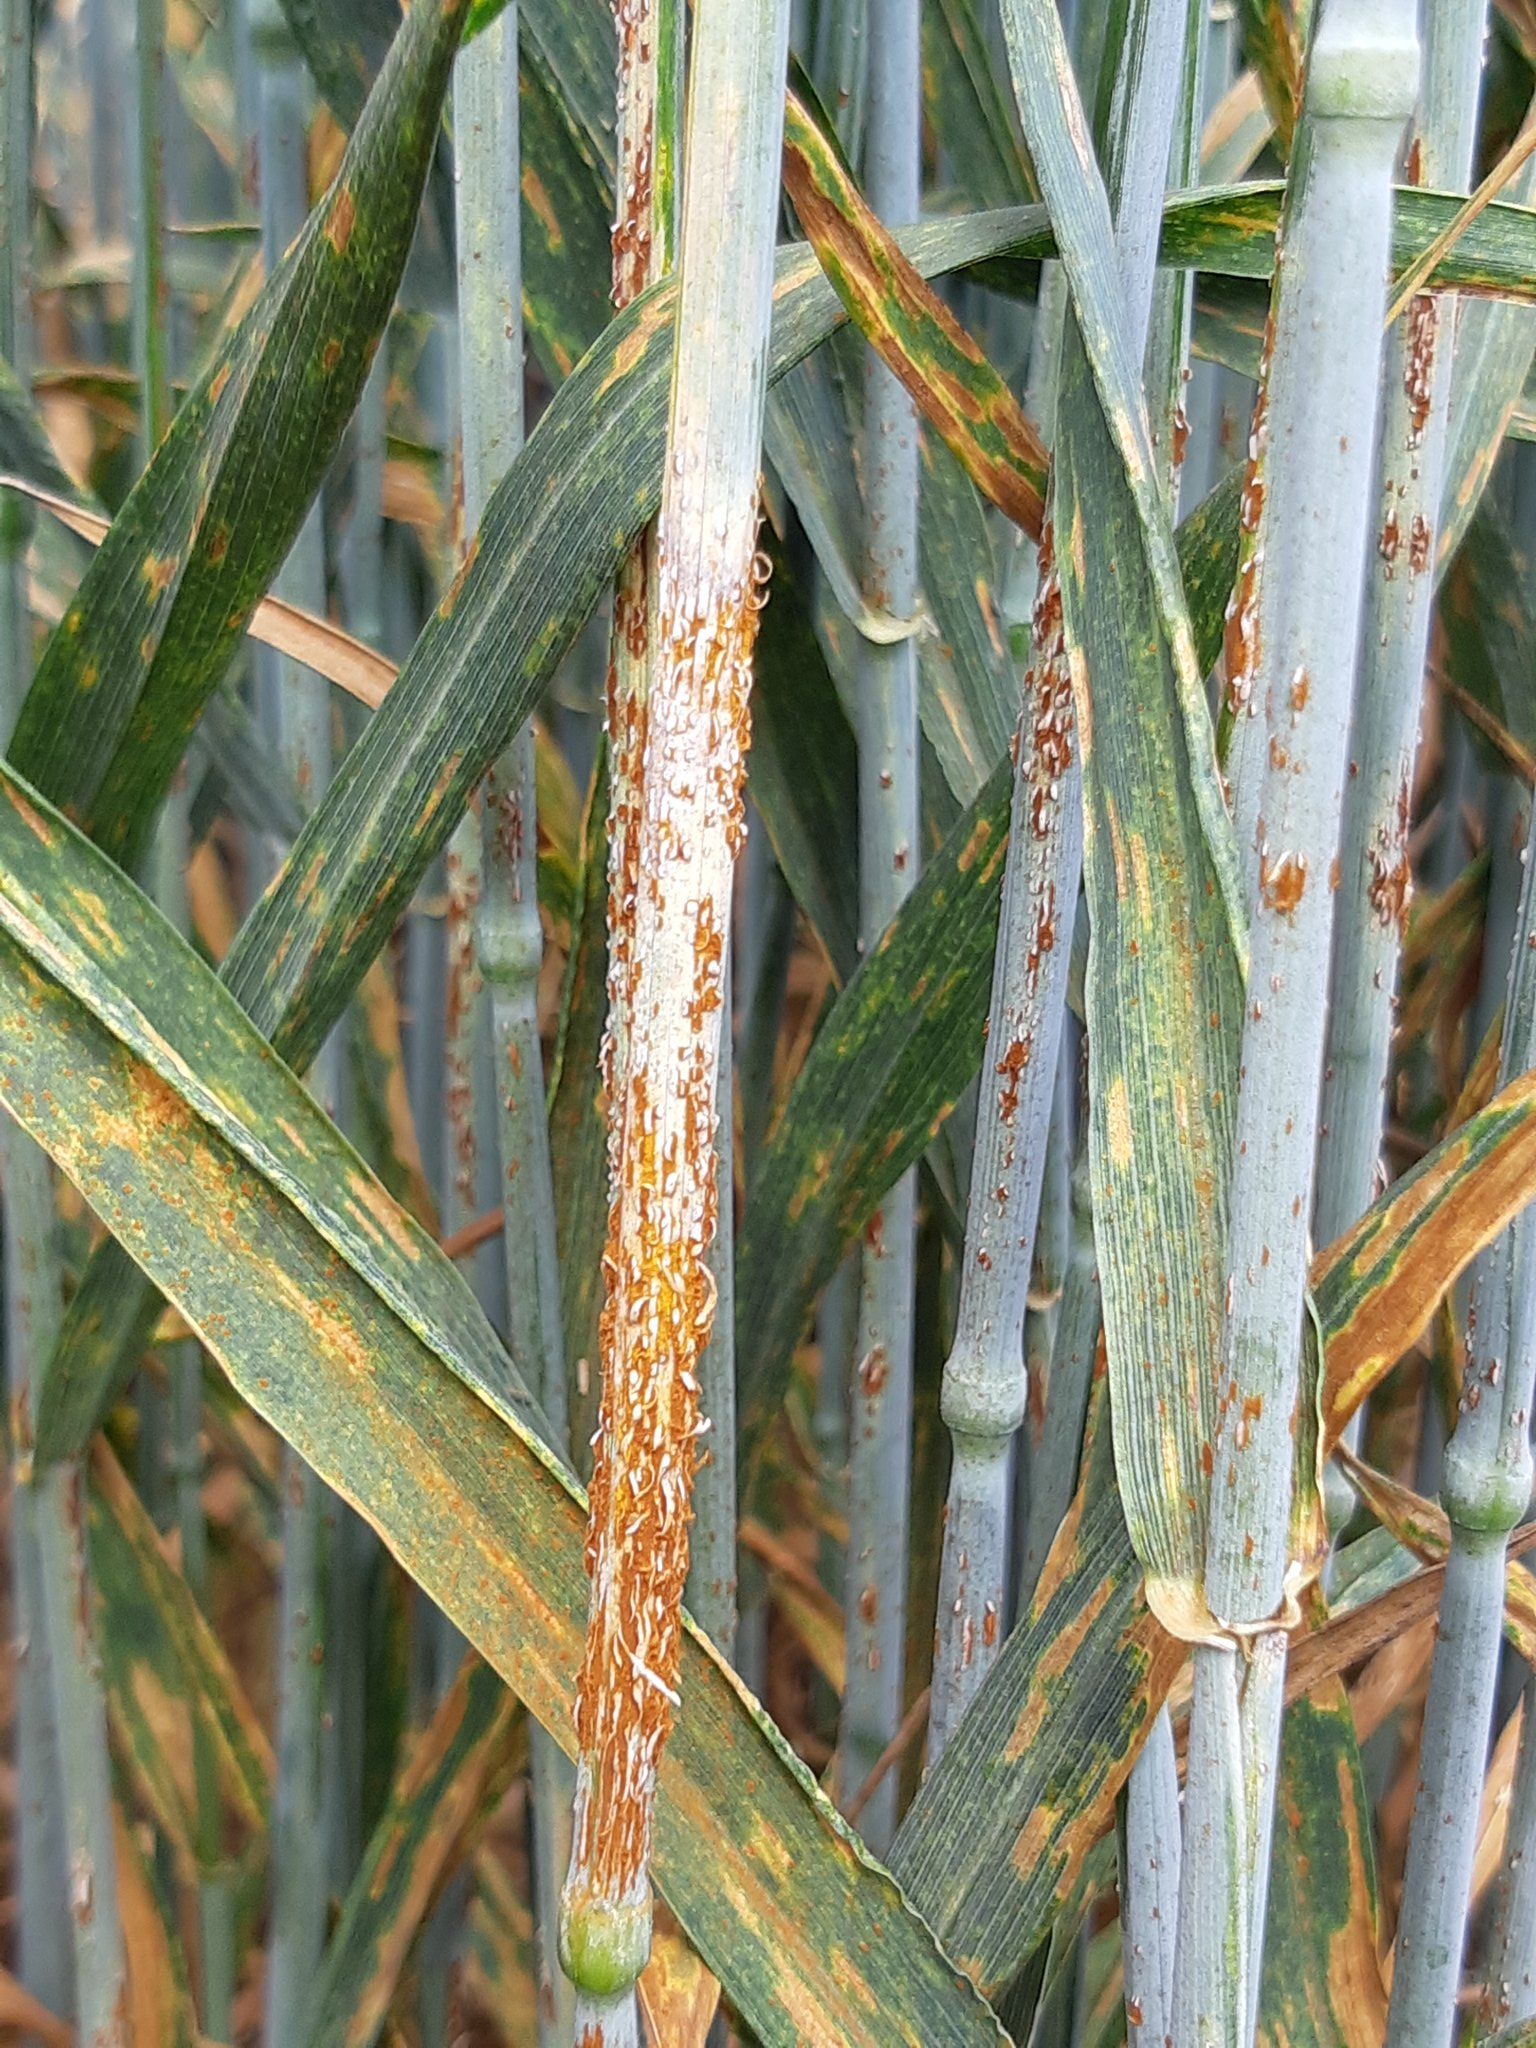
\includegraphics[width=0.55\linewidth]{../images/FWGDkkkWYAA3yF4} \end{center}

\end{columns}\end{figure}

\footnotesize

\begin{itemize}
\tightlist
\item
  Wheat stripe rust is an air-borne and destructive disease caused by a
  heteroecious rust fungus \textit{Puccinia striiformis }f.~sp.
  \textit{tritici} (Pst). Studies have demonstrated that the rust
  pathogen accomplishes sexual reproduction on susceptible barberry
  under natural conditions in spring, whereas Pst infection on barberry
  is still in blank in other seasons.
\end{itemize}
\end{frame}

\begin{frame}{}
\protect\hypertarget{section-12}{}
\begin{figure}\caption{\textit{Puccinia recondita} on \textit{Secale cereale}} 
\begin{columns}\column{0.4\textwidth}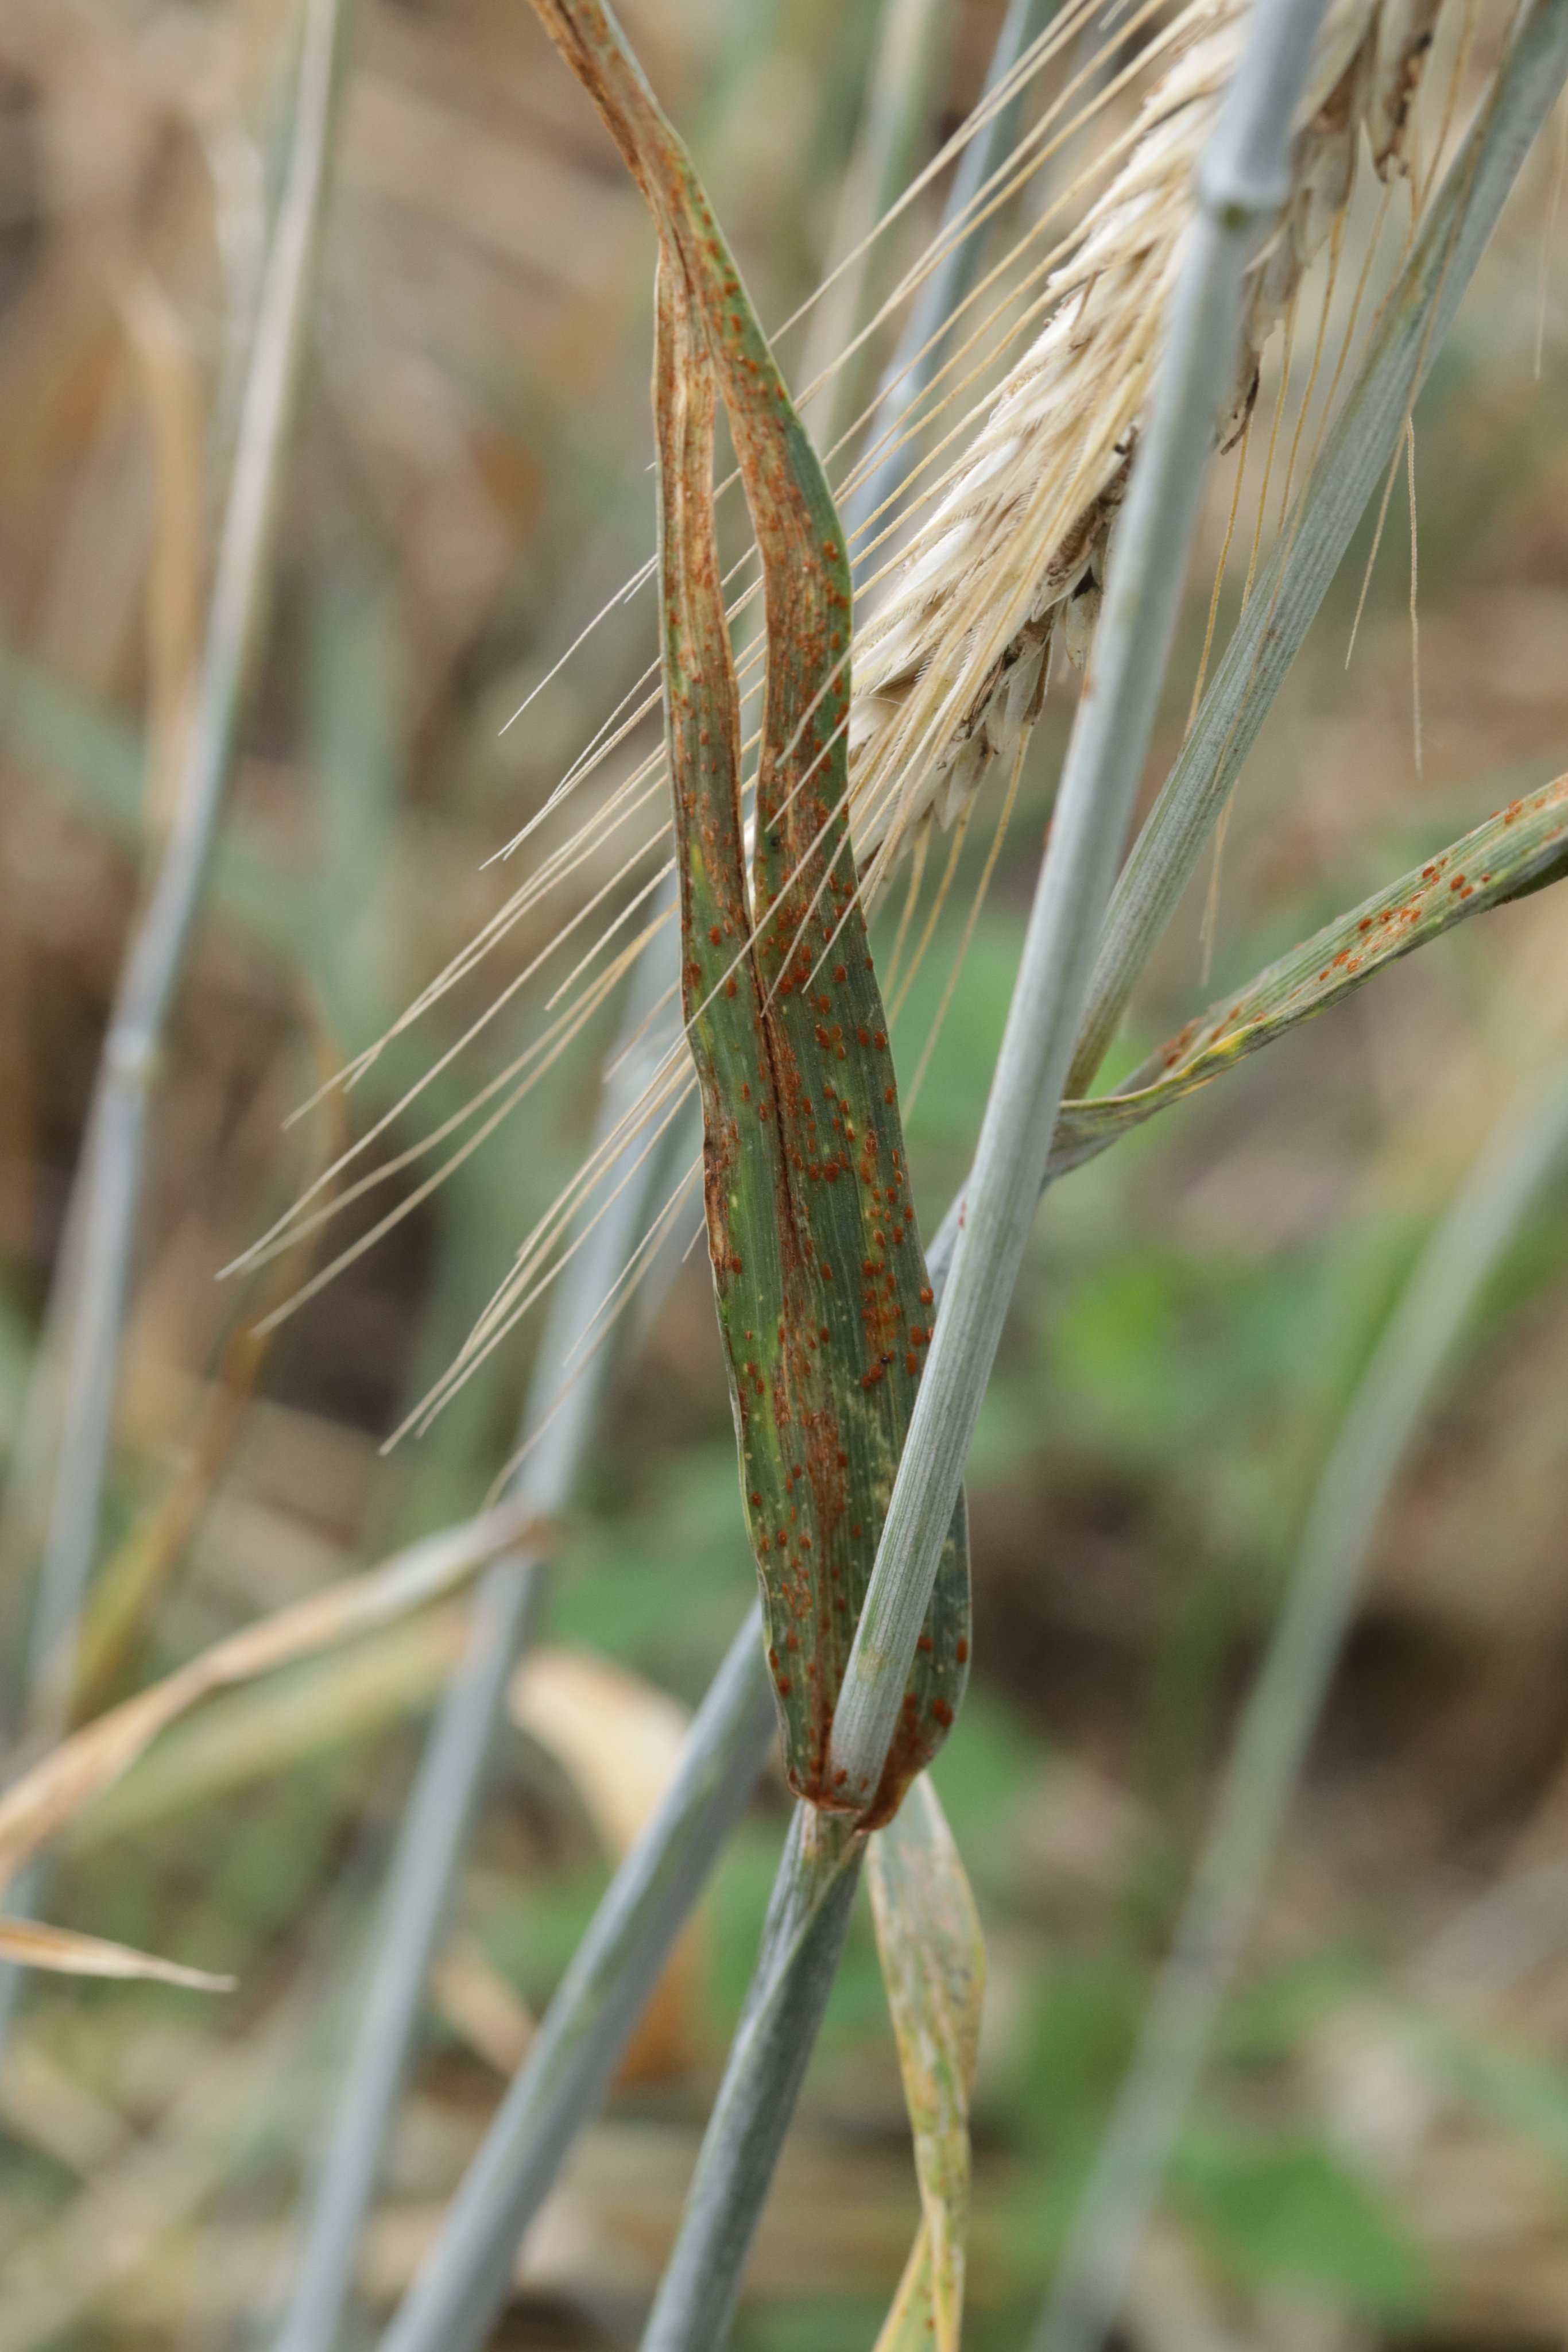
\includegraphics[width=0.72\linewidth]{../images/FYCo7NmWQAkXvRB}\column{0.6\textwidth}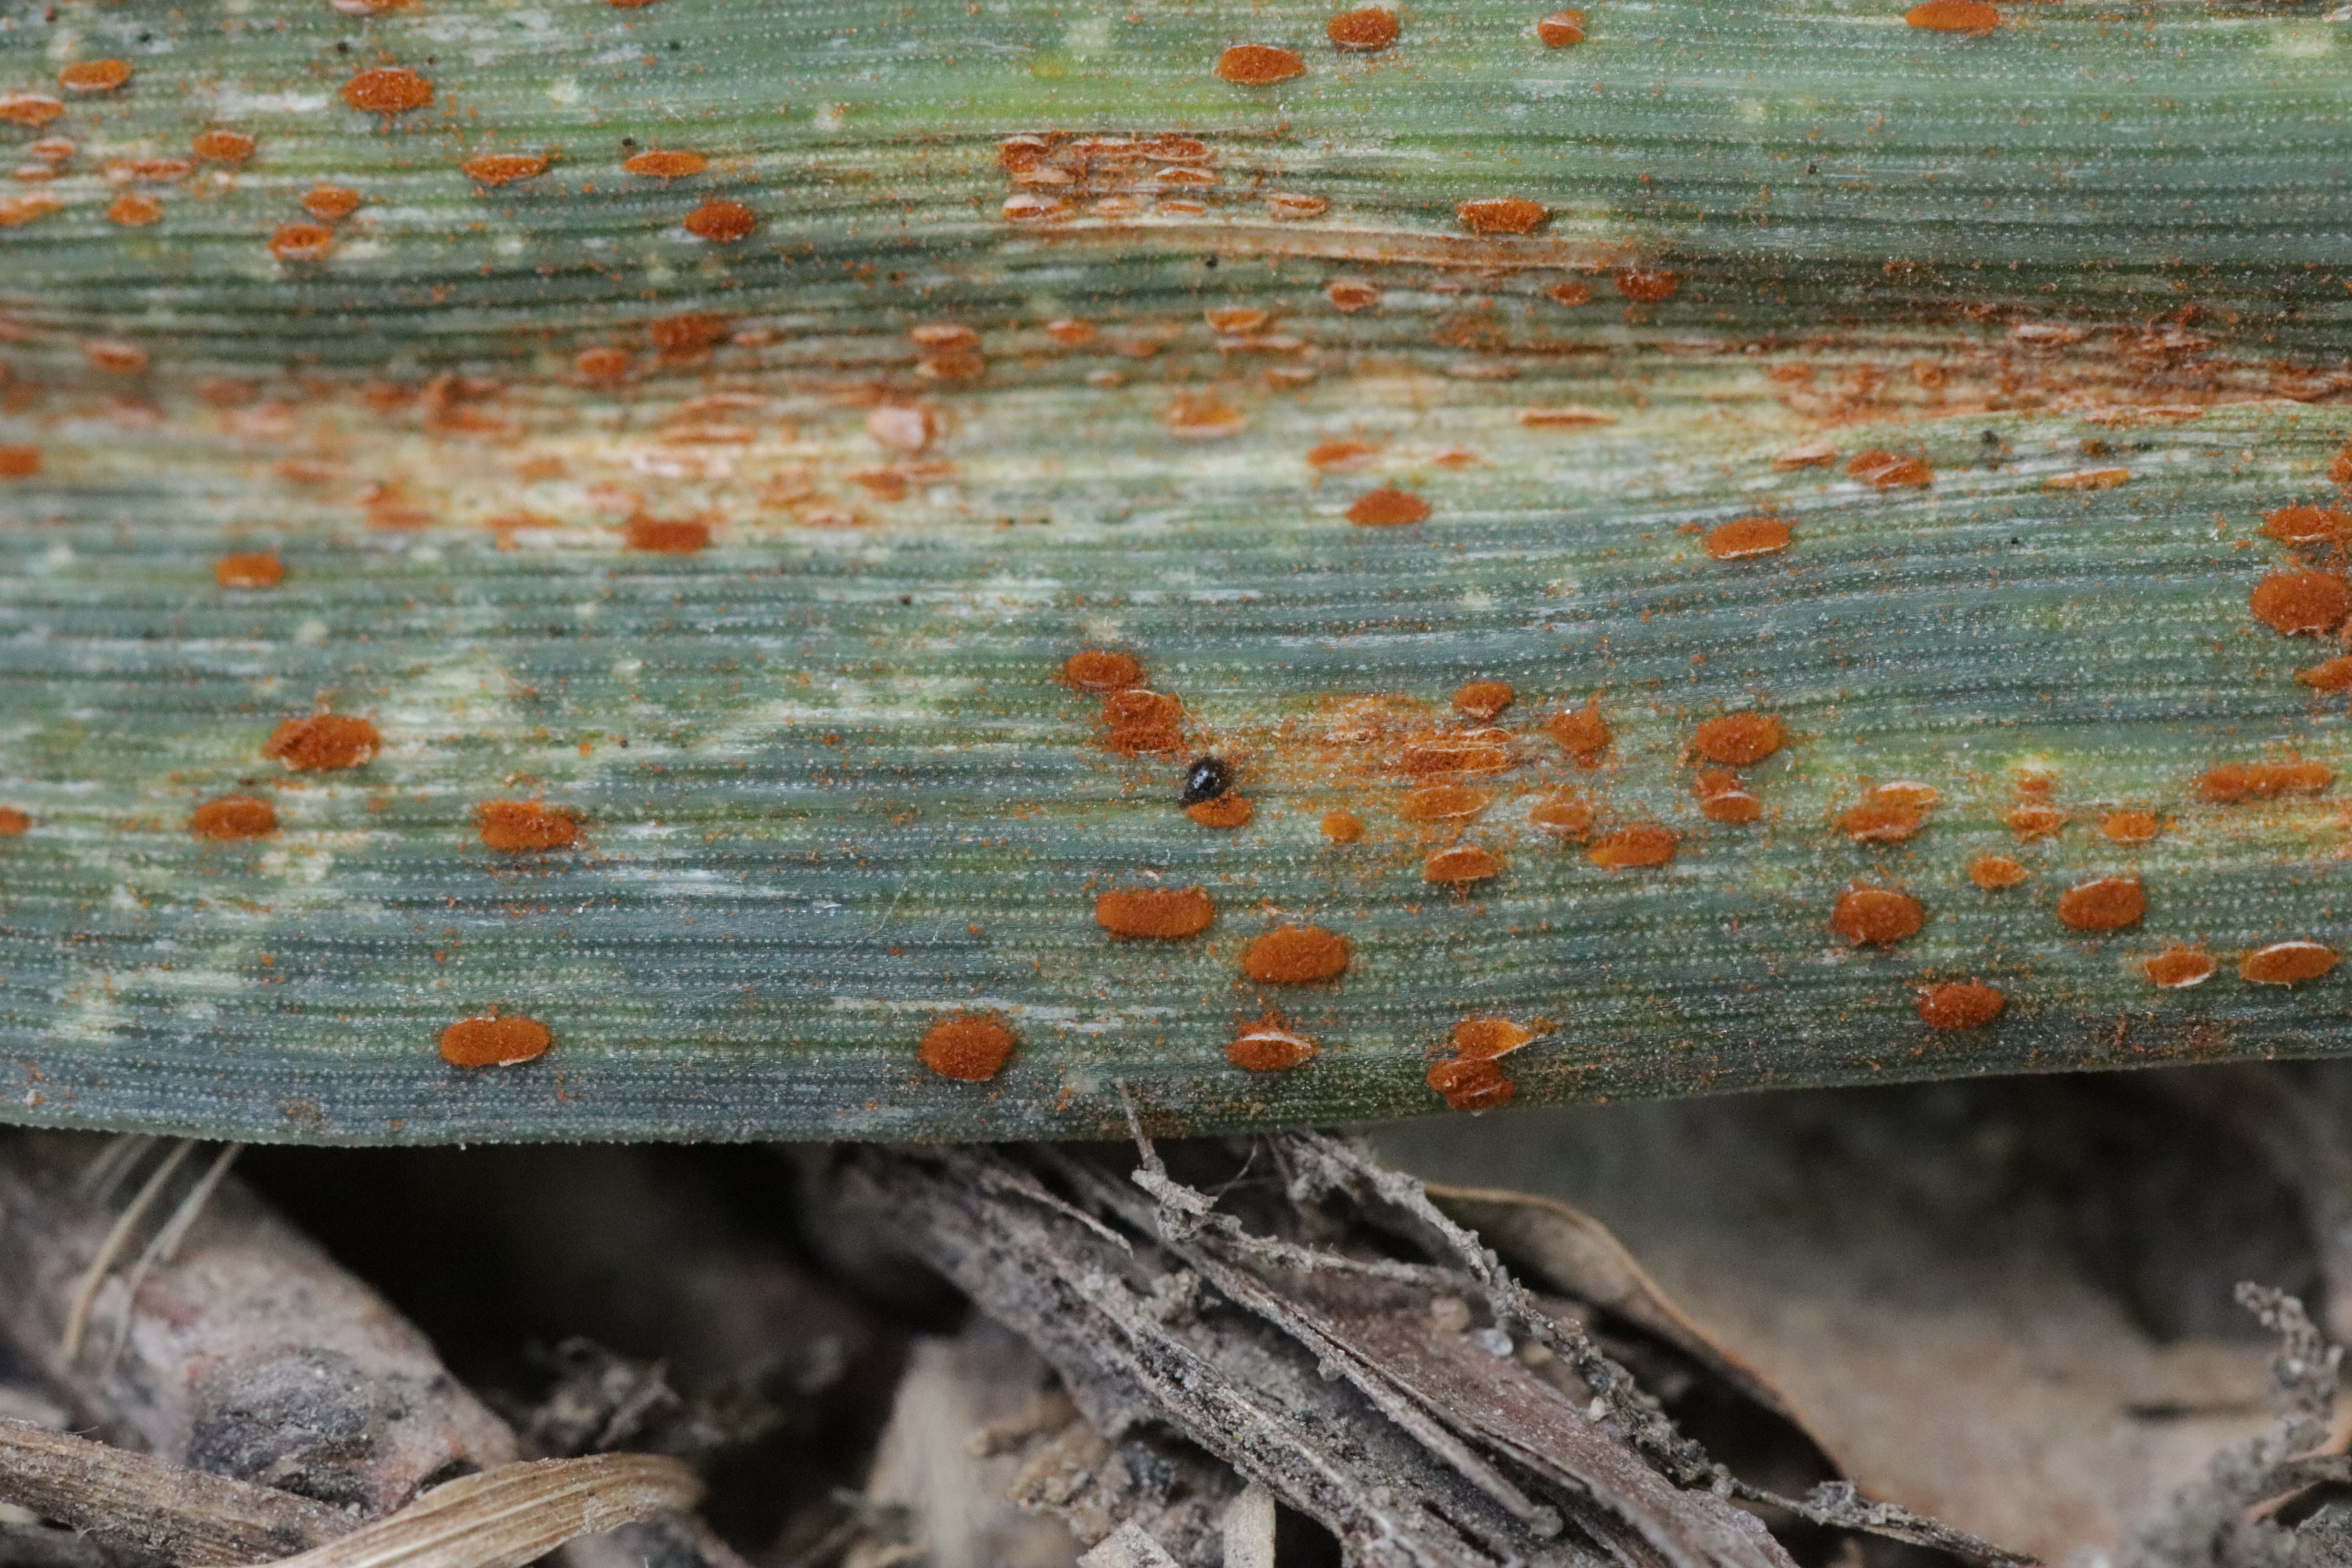
\includegraphics[width=0.6\linewidth]{../images/FYCo7NwXgAYe9r1} \\ 
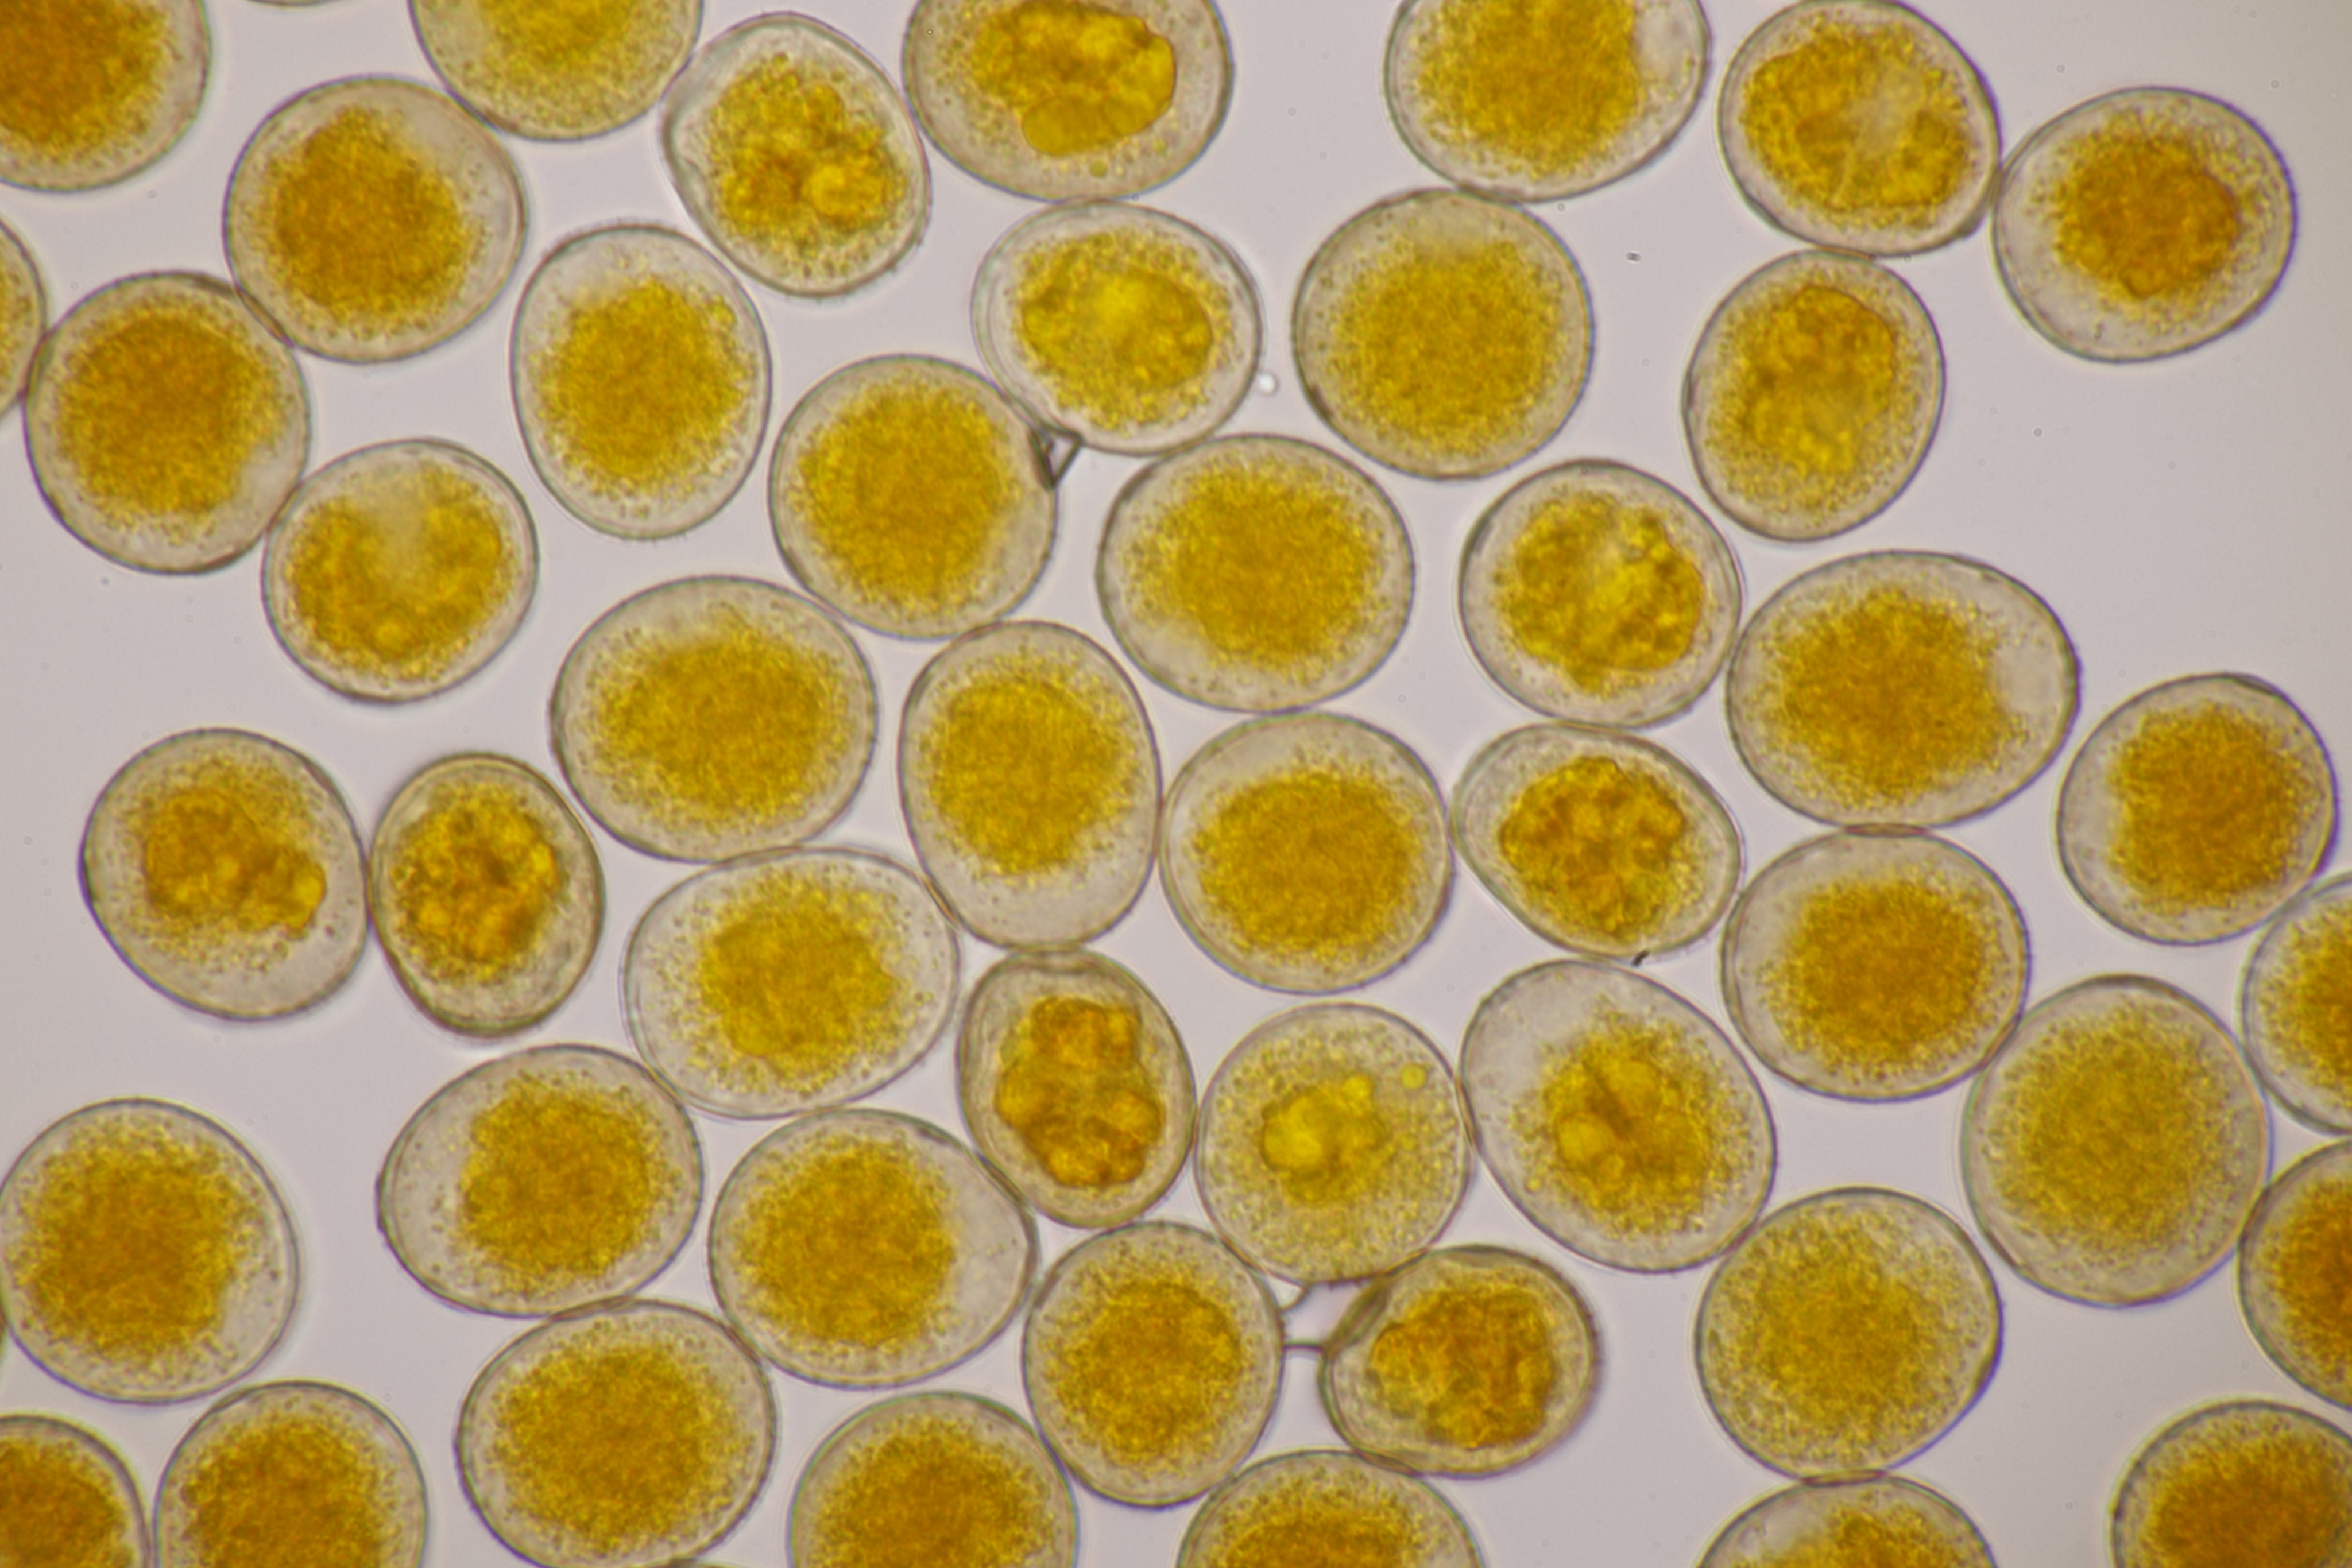
\includegraphics[width=0.6\linewidth]{../images/FYCo7NrXkAAOJZh}\end{columns}\end{figure}
\end{frame}

\begin{frame}{}
\protect\hypertarget{section-13}{}
\begin{figure}
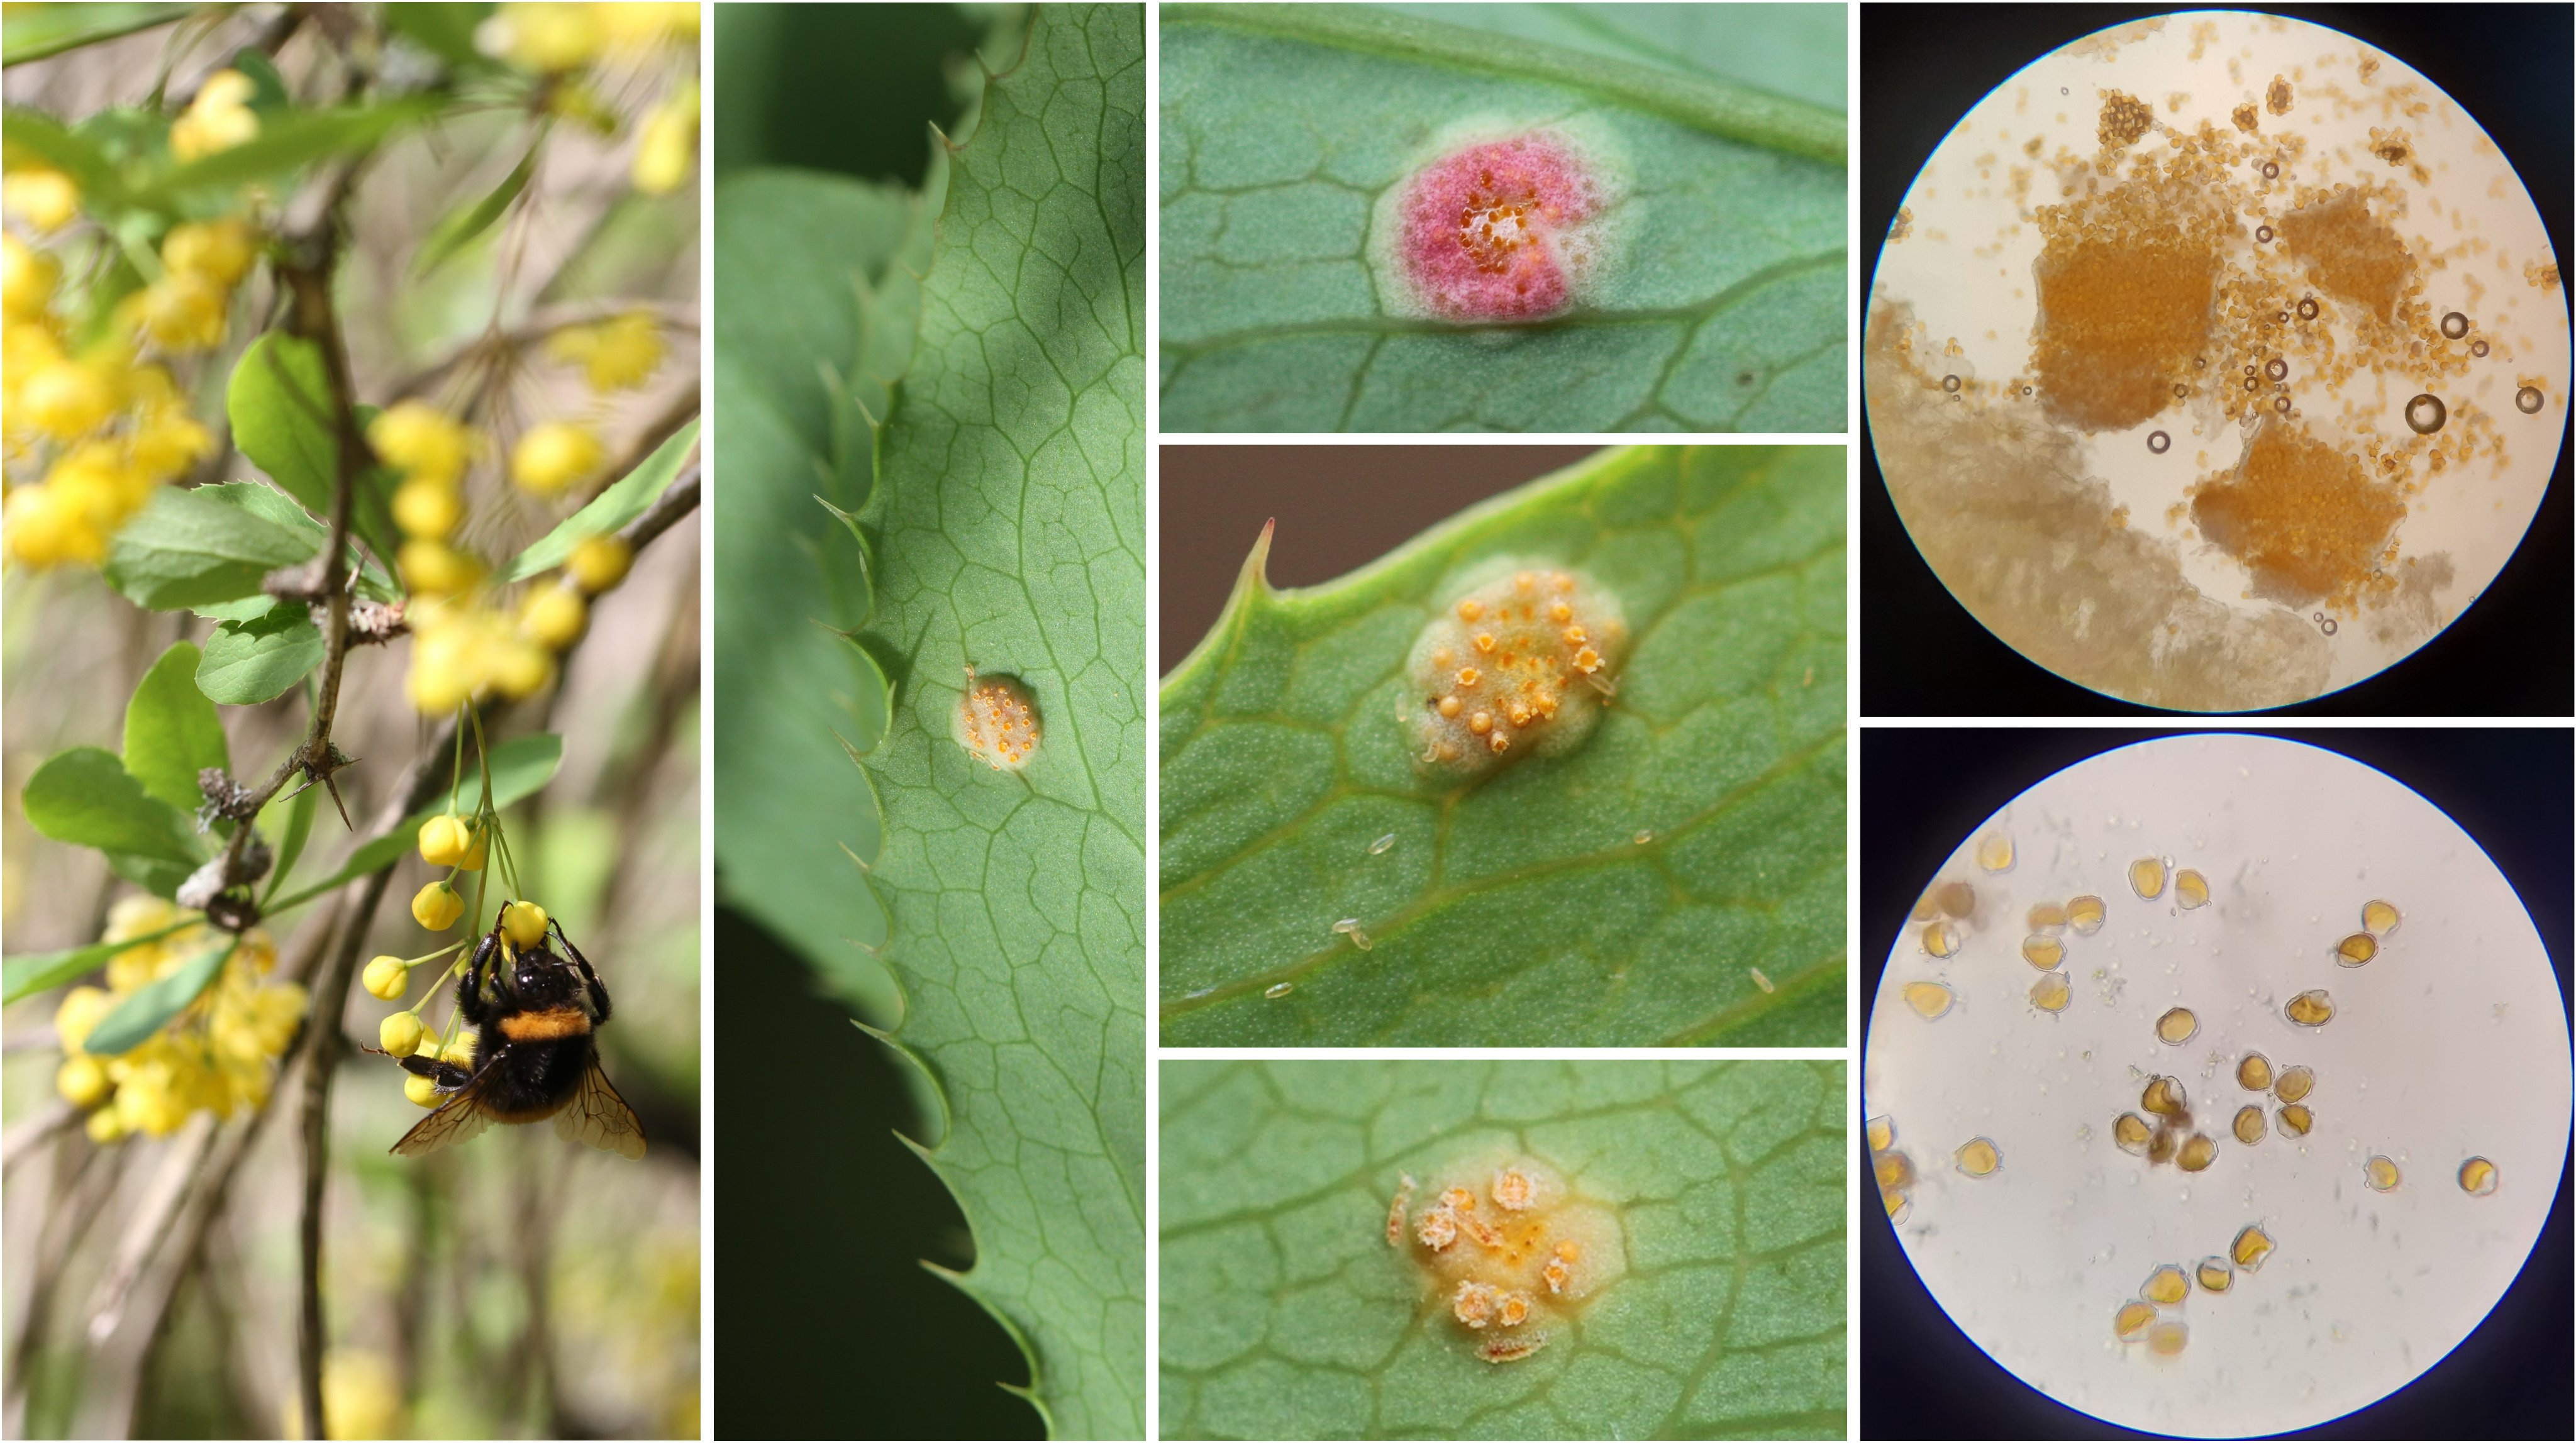
\includegraphics[width=0.36\linewidth]{../images/FRruRoiX0AE_dF0} \caption{Rust on flowering stage \textit{Berberis vulgaris} caused by \textit{Puccinia graminis} at the beginning of the aecial stage.}\label{fig:berberis-rust}
\end{figure}

\begin{figure}
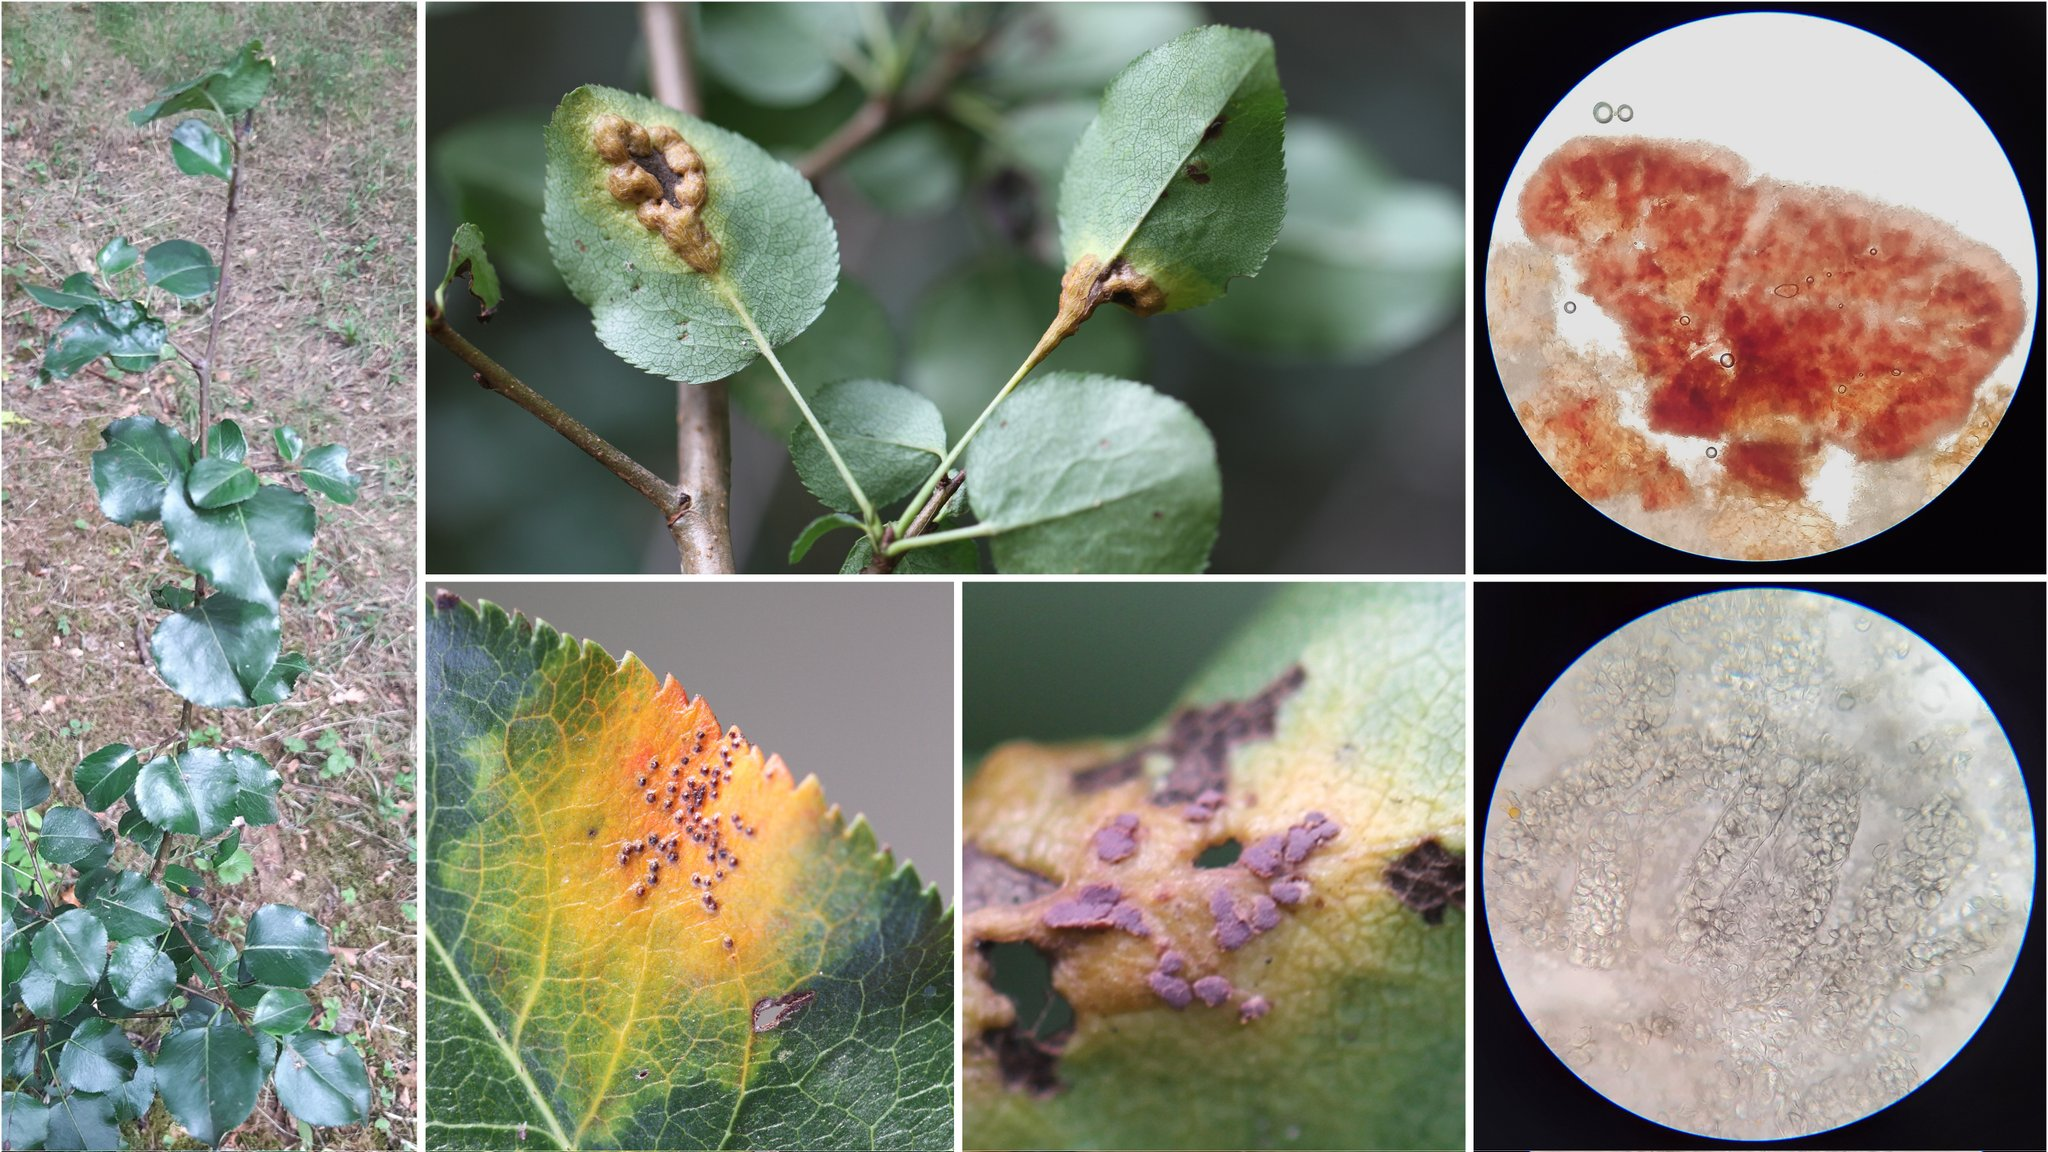
\includegraphics[width=0.38\linewidth]{../images/Fa1rQDGWAAAa8pu} \caption{Rust on a wild pear (\textit{Pyrus communis}) likely caused by \textit{Gymnosporangium sabinae}, here with a cluster of pycnia and pre-aecial tissues parasitized by \textit{Tuberculina} sp. (A hyperparasite) which is specific to Gymnosporangium.}\label{fig:pear-rust}
\end{figure}
\end{frame}

\begin{frame}{Fusarium}
\protect\hypertarget{fusarium}{}
\begin{itemize}
\tightlist
\item
  Fusariusm head blight/ear blight, foot rot, seedling blight Pathogen:
  \emph{Fusarium spp.} and \emph{Microdochium nivale}
\item
  Hosts: Wheat, barley, oats, rye triticale and grasses.
\item
  Symptoms

  \begin{itemize}
  \scriptsize
  \item Form a complex of diseases on seeds, seedlings and adult plants.
  \item \textit{Microdochium nivale} (formerly known as \textit{Fusarium nivale}) is seed-borne pathogen and causes seedling blight resulting in seedling death and thinning of plant stand.
  \item \textit{M}. spp (other than \textit{M. nivale}) cause a range of symptoms including brown lesions on stem bases, often restricted to outer leaf sheath.
  \item \textit{Fusarium lesions} often begin in the leaf sheath at the stem base where crown roots split the leaf sheath when emerging.
  \item This infection can spread up the leaf sheath causing long dark brown streaks at the stem base. The other symptom in cooler regions is brown staining of lower nodes.
  \item In older plants, fusarium infection can produce a true foot rot, where the stem base becomes brown and rotten, resulting in lodging and white heads.
  \item Symptoms are prevalent in very dry seasons as well.
  \item Ear blight causing fungus: \textit{F culmorum} and \textit{F graminearum} are common. Other are, \textit{F avenaceum}, \textit{F poae} and \textit{F langsethiae}.
  \item Infection frequently results in the whole or part of the ear becoming bleached.
  \item Symptoms seen when ears become infected during the early flowering stages, later infection may result in infection of grain but without obvious bleaching of the ears.
  \item Important due to its mycotoxin that gets accumulated in grains.
  \end{itemize}
\end{itemize}
\end{frame}

\begin{frame}{Fusarium: Life cycle}
\protect\hypertarget{fusarium-life-cycle}{}
\begin{itemize}
\tightlist
\item
  Most important source is seed but fungus survives on debris in soil
  also.
\item
  Spores are splashed in canopy causing ear blights and seed borne
  infection, in wet seasons, especially during flowering and grain
  formation.
\item
  Most fusarium species have competative saprophytic abilities which
  allow them to colonize debris and stubble in soil.
\item
  Importance:

  \begin{itemize}
  \tightlist
  \item
    When wet season coincides with flowering high levels of ear blight
    can occur.
  \item
    Due to seed borne nature of pathogen, seed treatment plays role in
    preventing seedling loss in wheat.
  \end{itemize}
\end{itemize}
\end{frame}

\begin{frame}{}
\protect\hypertarget{section-14}{}
\begin{figure}
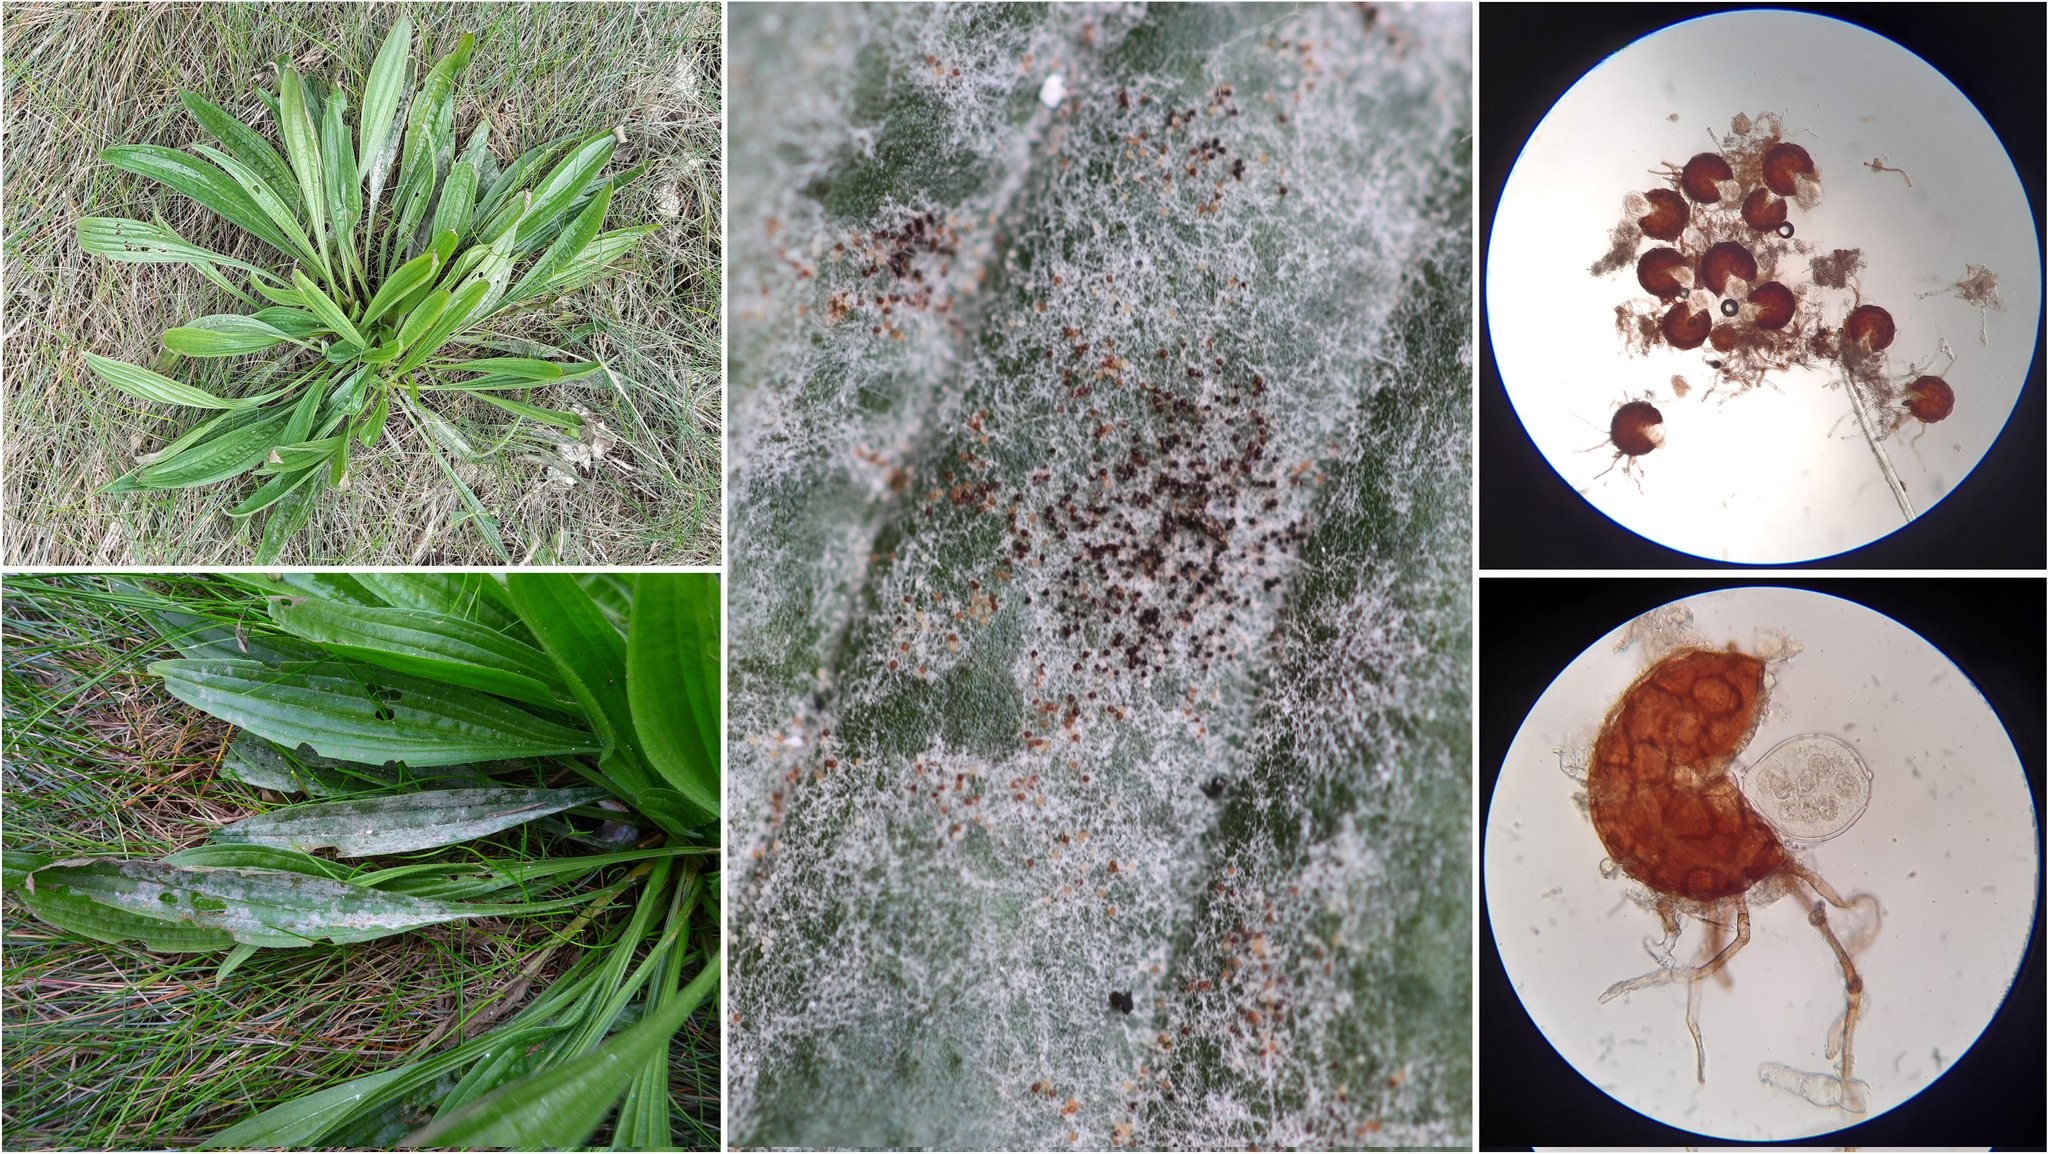
\includegraphics[width=0.38\linewidth]{../images/plantain_podosphaera_plantaginis_powdery_mildew} \caption{Powdery mildew on buckhorn plantain (\textit{Plantago lanceolata}) caused by \textit{Podosphaera plantaginis}, here with cleistothecia containing a single ascus and eight ascospores.}\label{fig:plantain-powdery-mildew}
\end{figure}

\begin{figure}
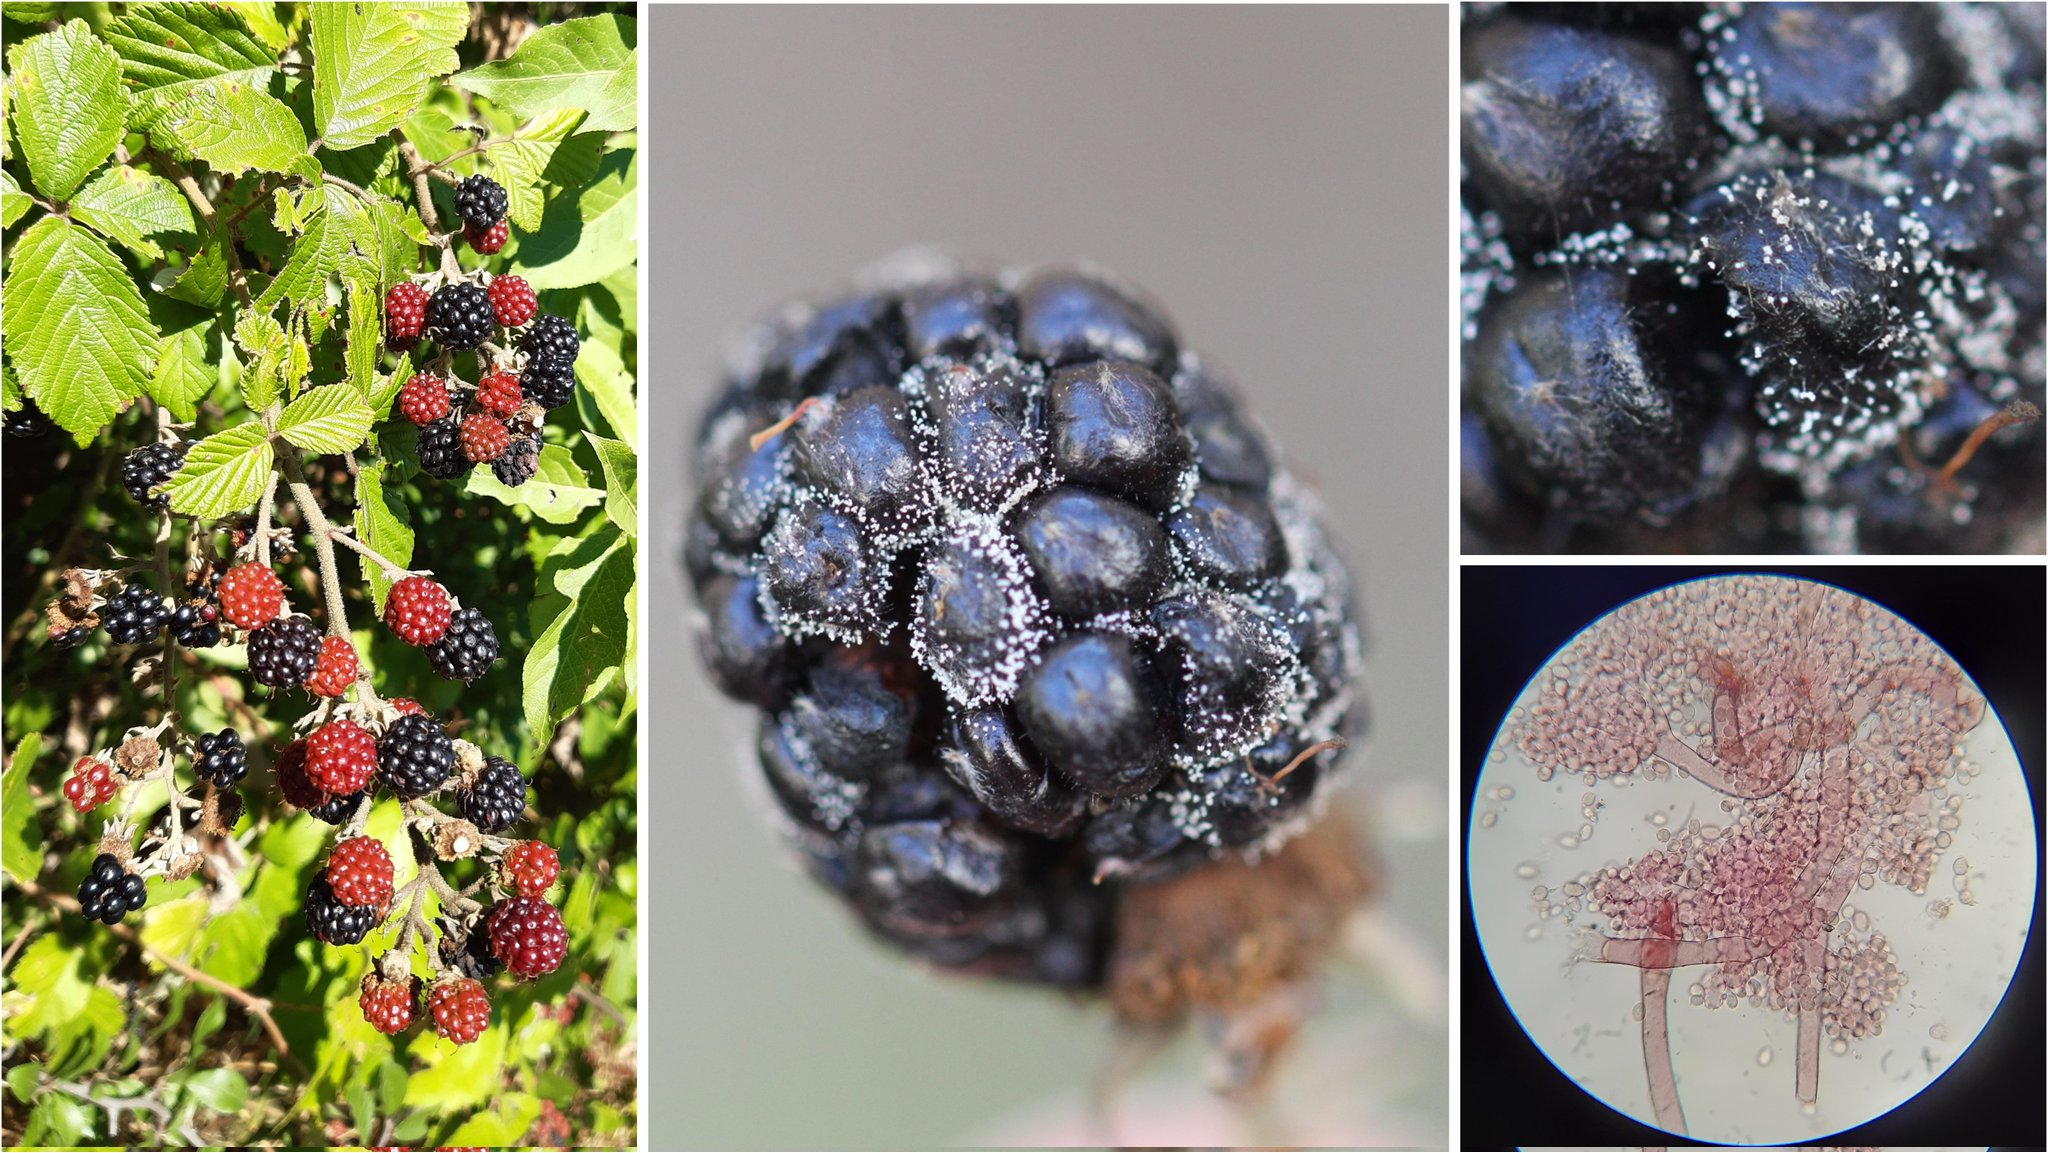
\includegraphics[width=0.38\linewidth]{../images/blackberry_botrytis_rot} \caption{Botrytis fruit rot on blackberry (\textit{Rubus fruticosus}).}\label{fig:blackberry-botrytis-rot}
\end{figure}
\end{frame}

\begin{frame}{}
\protect\hypertarget{section-15}{}
\begin{columns}[T, onlytextwidth]
\column{0.5\textwidth}

\begin{figure}
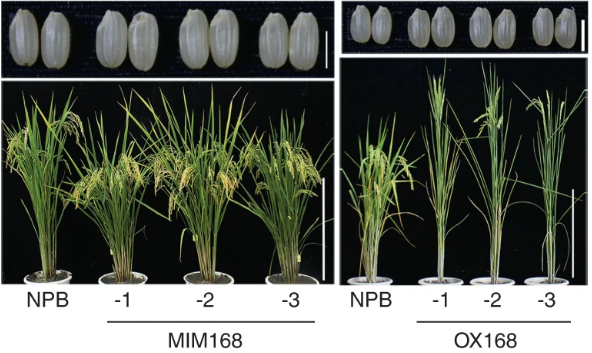
\includegraphics[width=0.9\linewidth]{../images/suppression_rice_miR168} \caption{Suppression of rice miR168 improves yield, flowering time and immunity against rice blast using a target mimic approach.}\label{fig:rice-blast-tolerance}
\end{figure}

\column{0.5\textwidth}

\begin{figure}
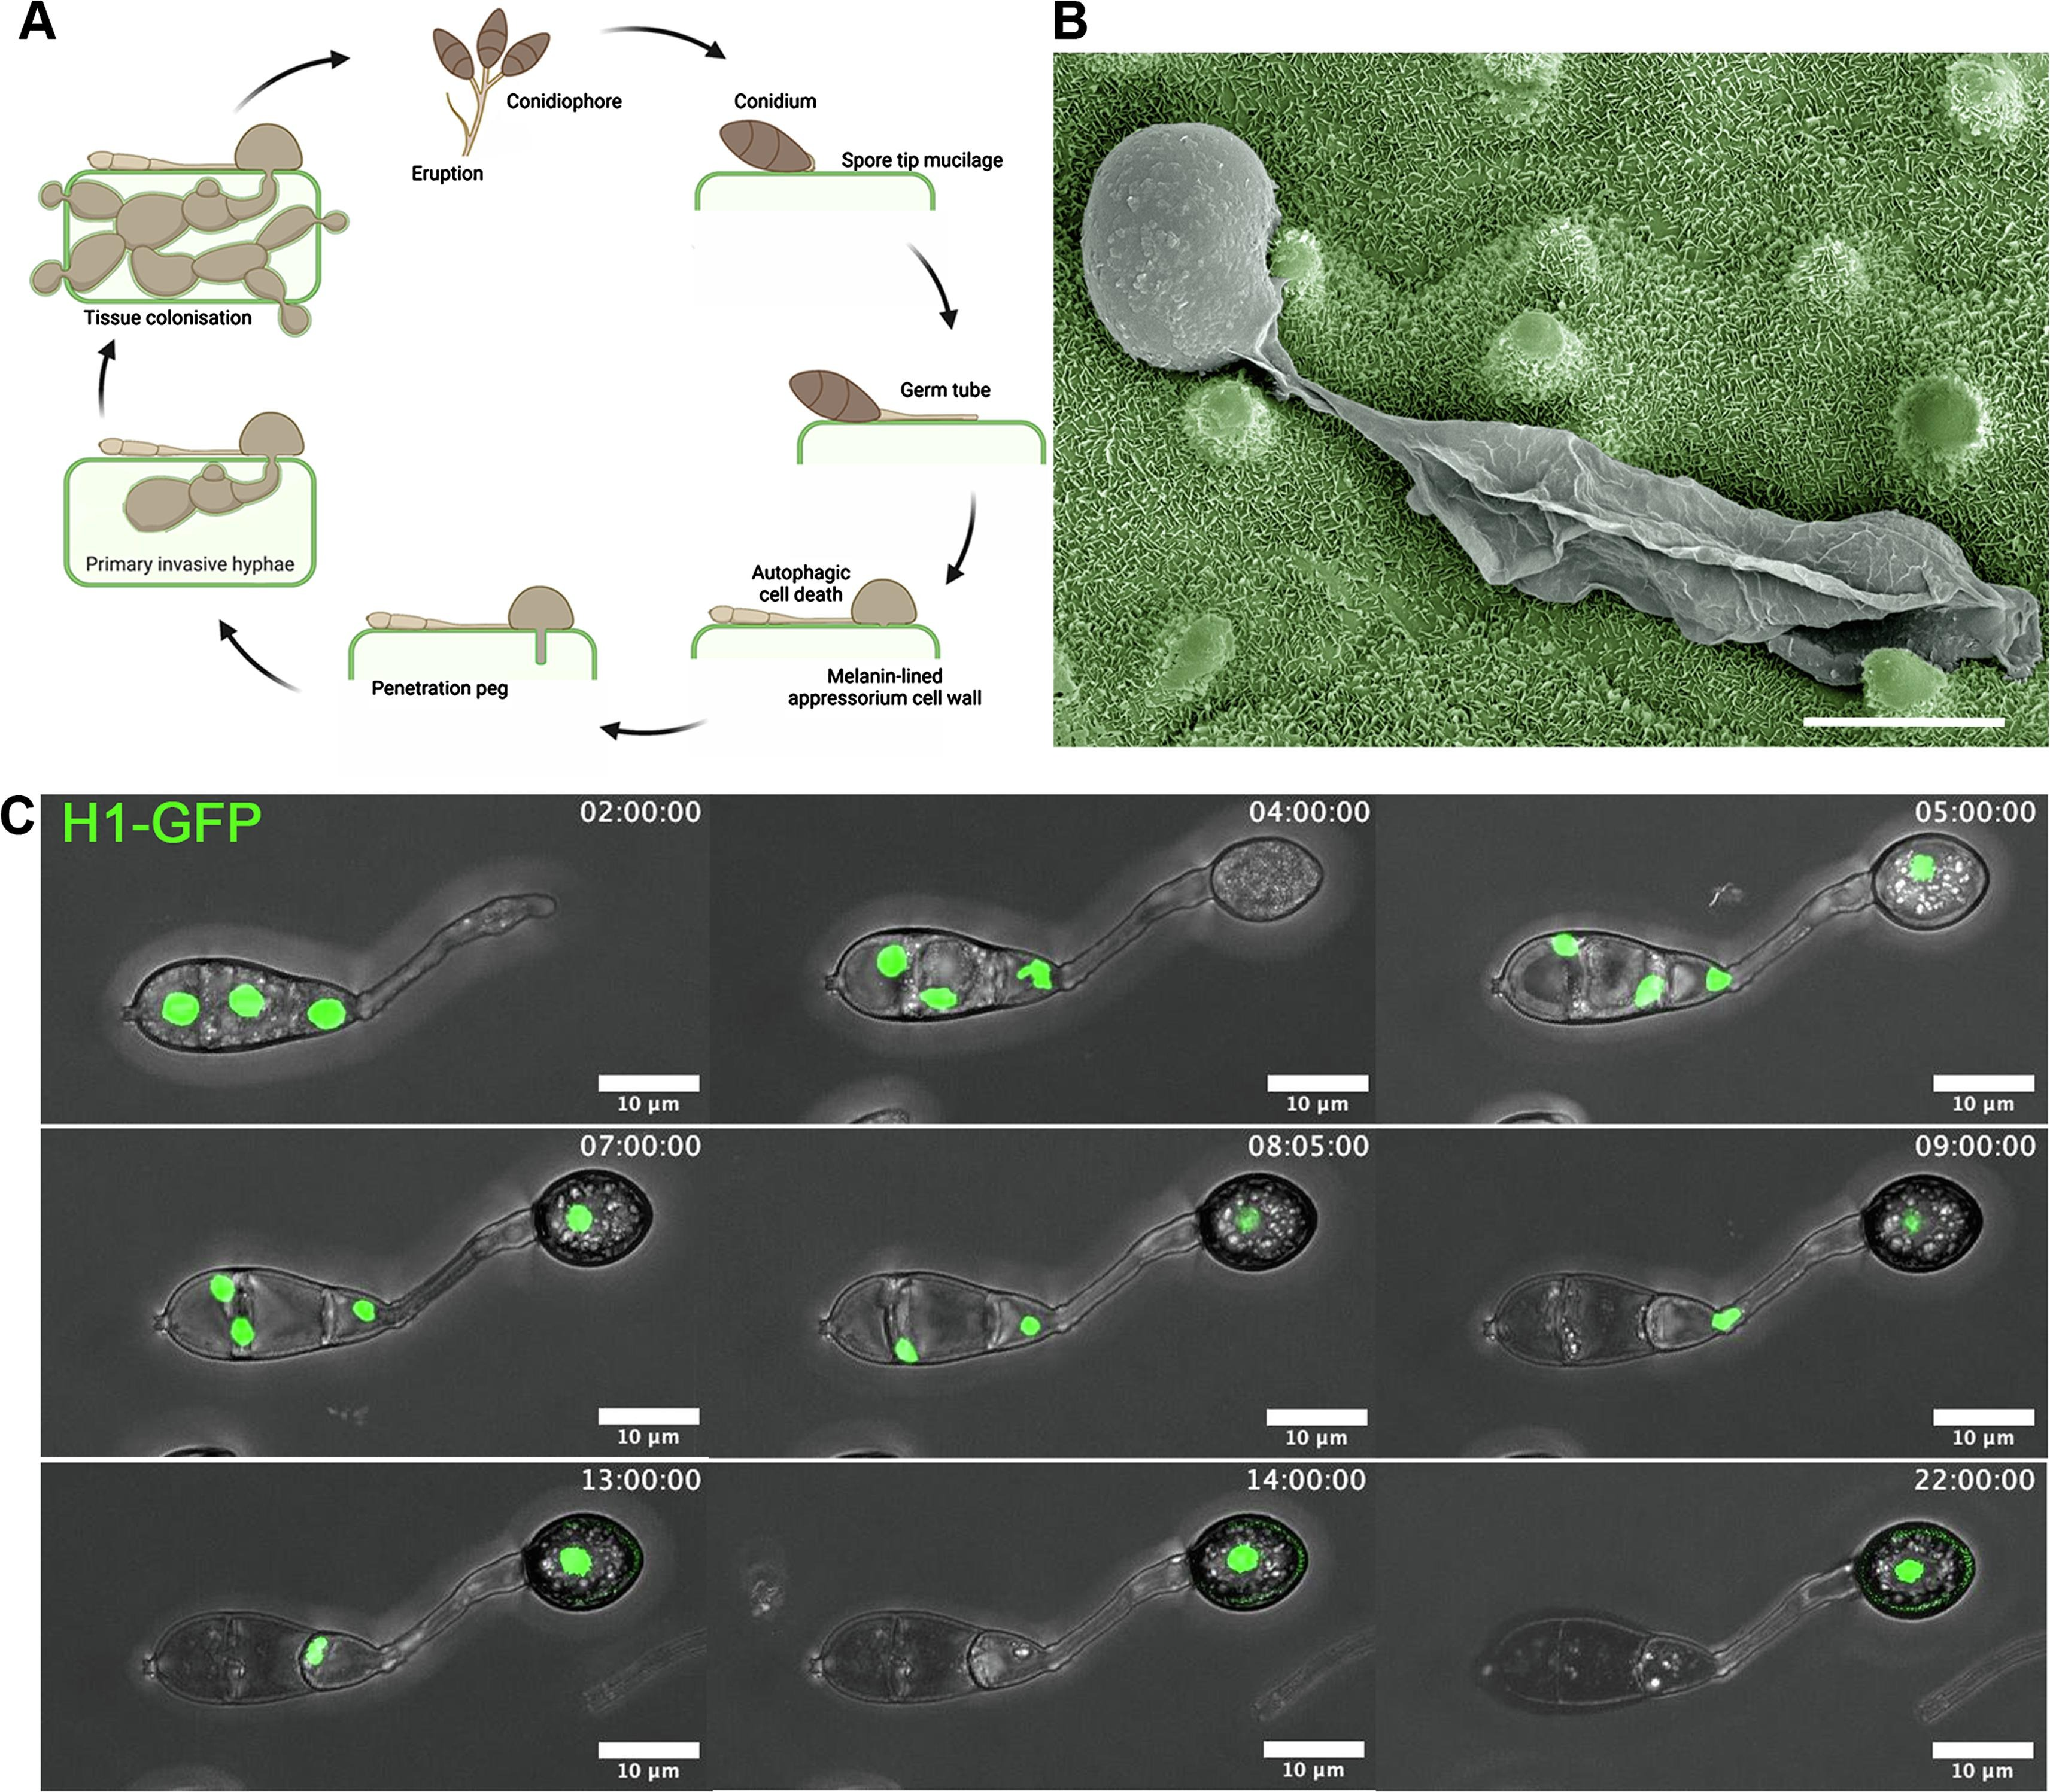
\includegraphics[width=0.9\linewidth]{../images/biology_rice_blast_magnaporthe_infection} \caption{Cell and developmental biology of plant infection by rice blast fungus \textit{Magnaporthe oryzae}.}\label{fig:rice-blast-biology}
\end{figure}

\end{columns}

\footnotesize Note: For cell and developmental biology of infection by
blast fungus, refer to \citet{eseola2021investigating}.
\end{frame}

\begin{frame}{}
\protect\hypertarget{section-16}{}
\begin{columns}[T, onlytextwidth]
\column{0.45\textwidth}

\begin{figure}
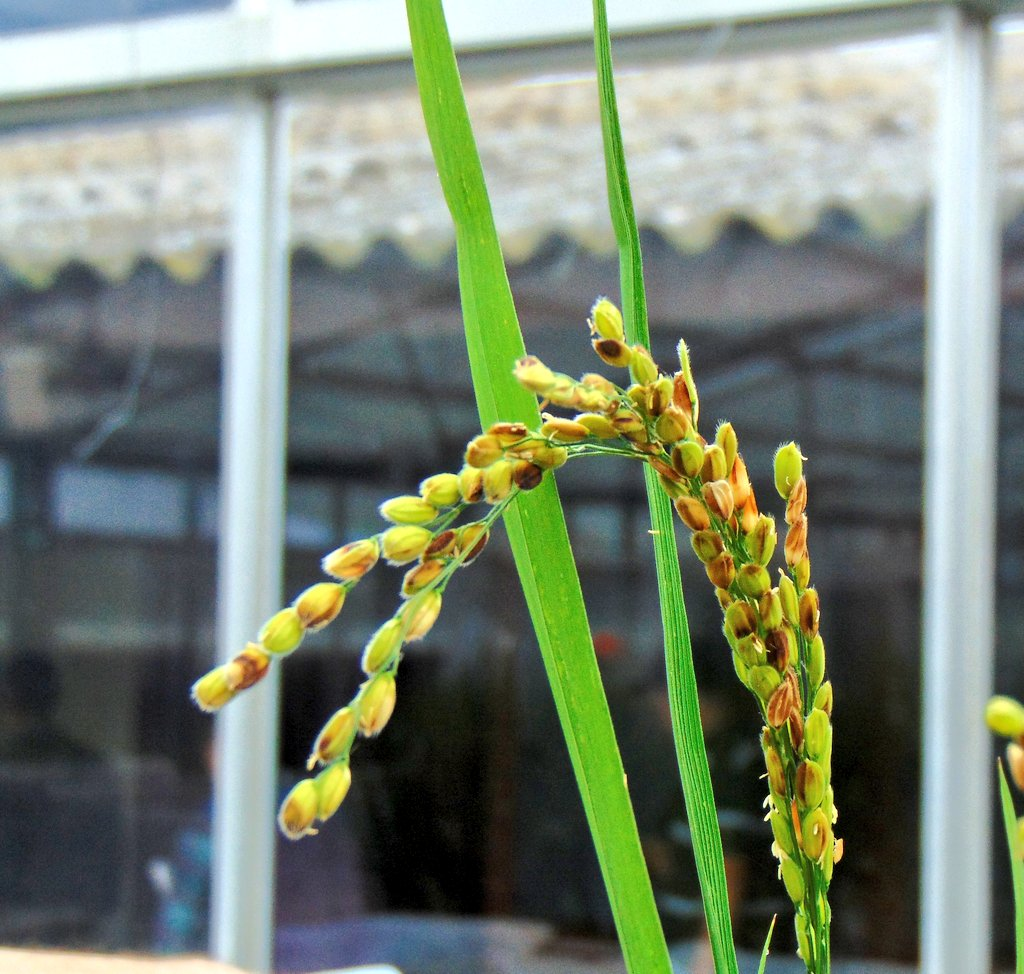
\includegraphics[width=0.84\linewidth]{../images/panicle_bast_rice} \caption{Panicle blast of rice caused by \textit{Burkholderia glumae}}\label{fig:rice-panicle-blast}
\end{figure}

\column{0.55\textwidth}

\begin{figure}
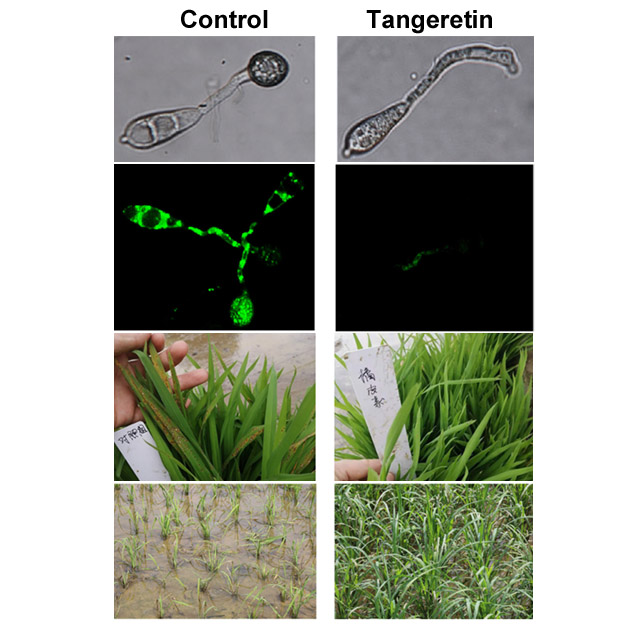
\includegraphics[width=0.85\linewidth]{../images/citrus_peel_for_blast_control} \caption{Tangeretin, an antioxidant commonly found in citrus peels, is a powerful antifungal in the fight against rice blast disease.}\label{fig:citrus-peel-rescuse}
\end{figure}

\end{columns}

\footnotesize Refer to \citet{liang2021tangeretin} on use of antioxidant
against rice blast fungus.
\end{frame}

\begin{frame}{}
\protect\hypertarget{section-17}{}
\begin{figure}
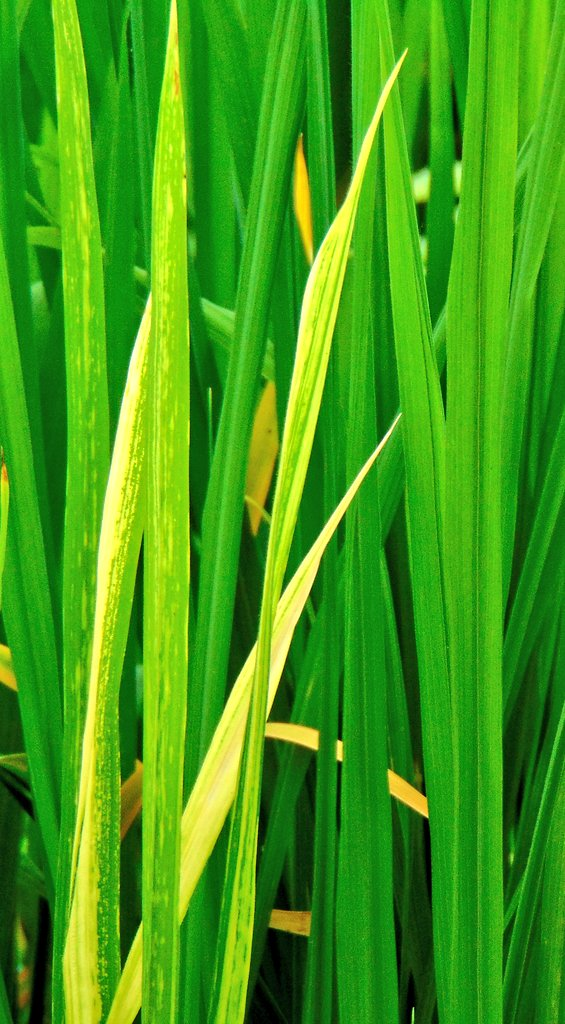
\includegraphics[width=0.25\linewidth]{../images/rice_hoja_blanca_virus} \caption{Rice hoja blanca virus}\label{fig:rice-hoja-blanca-virus}
\end{figure}
\end{frame}

\hypertarget{mechanisms-of-infection}{%
\section{Mechanisms of infection}\label{mechanisms-of-infection}}

\begin{frame}{Mechanisms of infection}
\footnotesize

\begin{itemize}
\tightlist
\item
  Pathogens act in a variety of pathways to cause infection
\item
  In pathogens that show a high level of gene flow, greater genetic
  diversity exists
\item
  In pathogens reproducing asexually (with no recombination), entire
  genotypes are transferred from one population to another -- phenomena
  called genotype flow
\item
  Hardy spores or propagules (rust and powdery mildew) can spread over
  long distances, sometimes encompassing entire continents.
\item
  Soil-borne fungi and nematodes move slowly and are present in small
  areas.
\item
  Gene flow reduces genetic differences between populations, preventing
  delays in drastic evolution of the population in different
  geographical areas.
\item
  Population size affects phenomena such as mutation, genetic drift and
  selection

  \begin{itemize}
  \footnotesize
  \item $\Uparrow$ population size $\thicksim$ $\Uparrow$ mutants alleles are conserved
  \item $\Uparrow$ population size $\thicksim$ $\Uparrow$ rare alleles are preserved under genetic drift 
  \end{itemize}
\end{itemize}
\end{frame}

\begin{frame}{}
\protect\hypertarget{section-18}{}
\begin{figure}
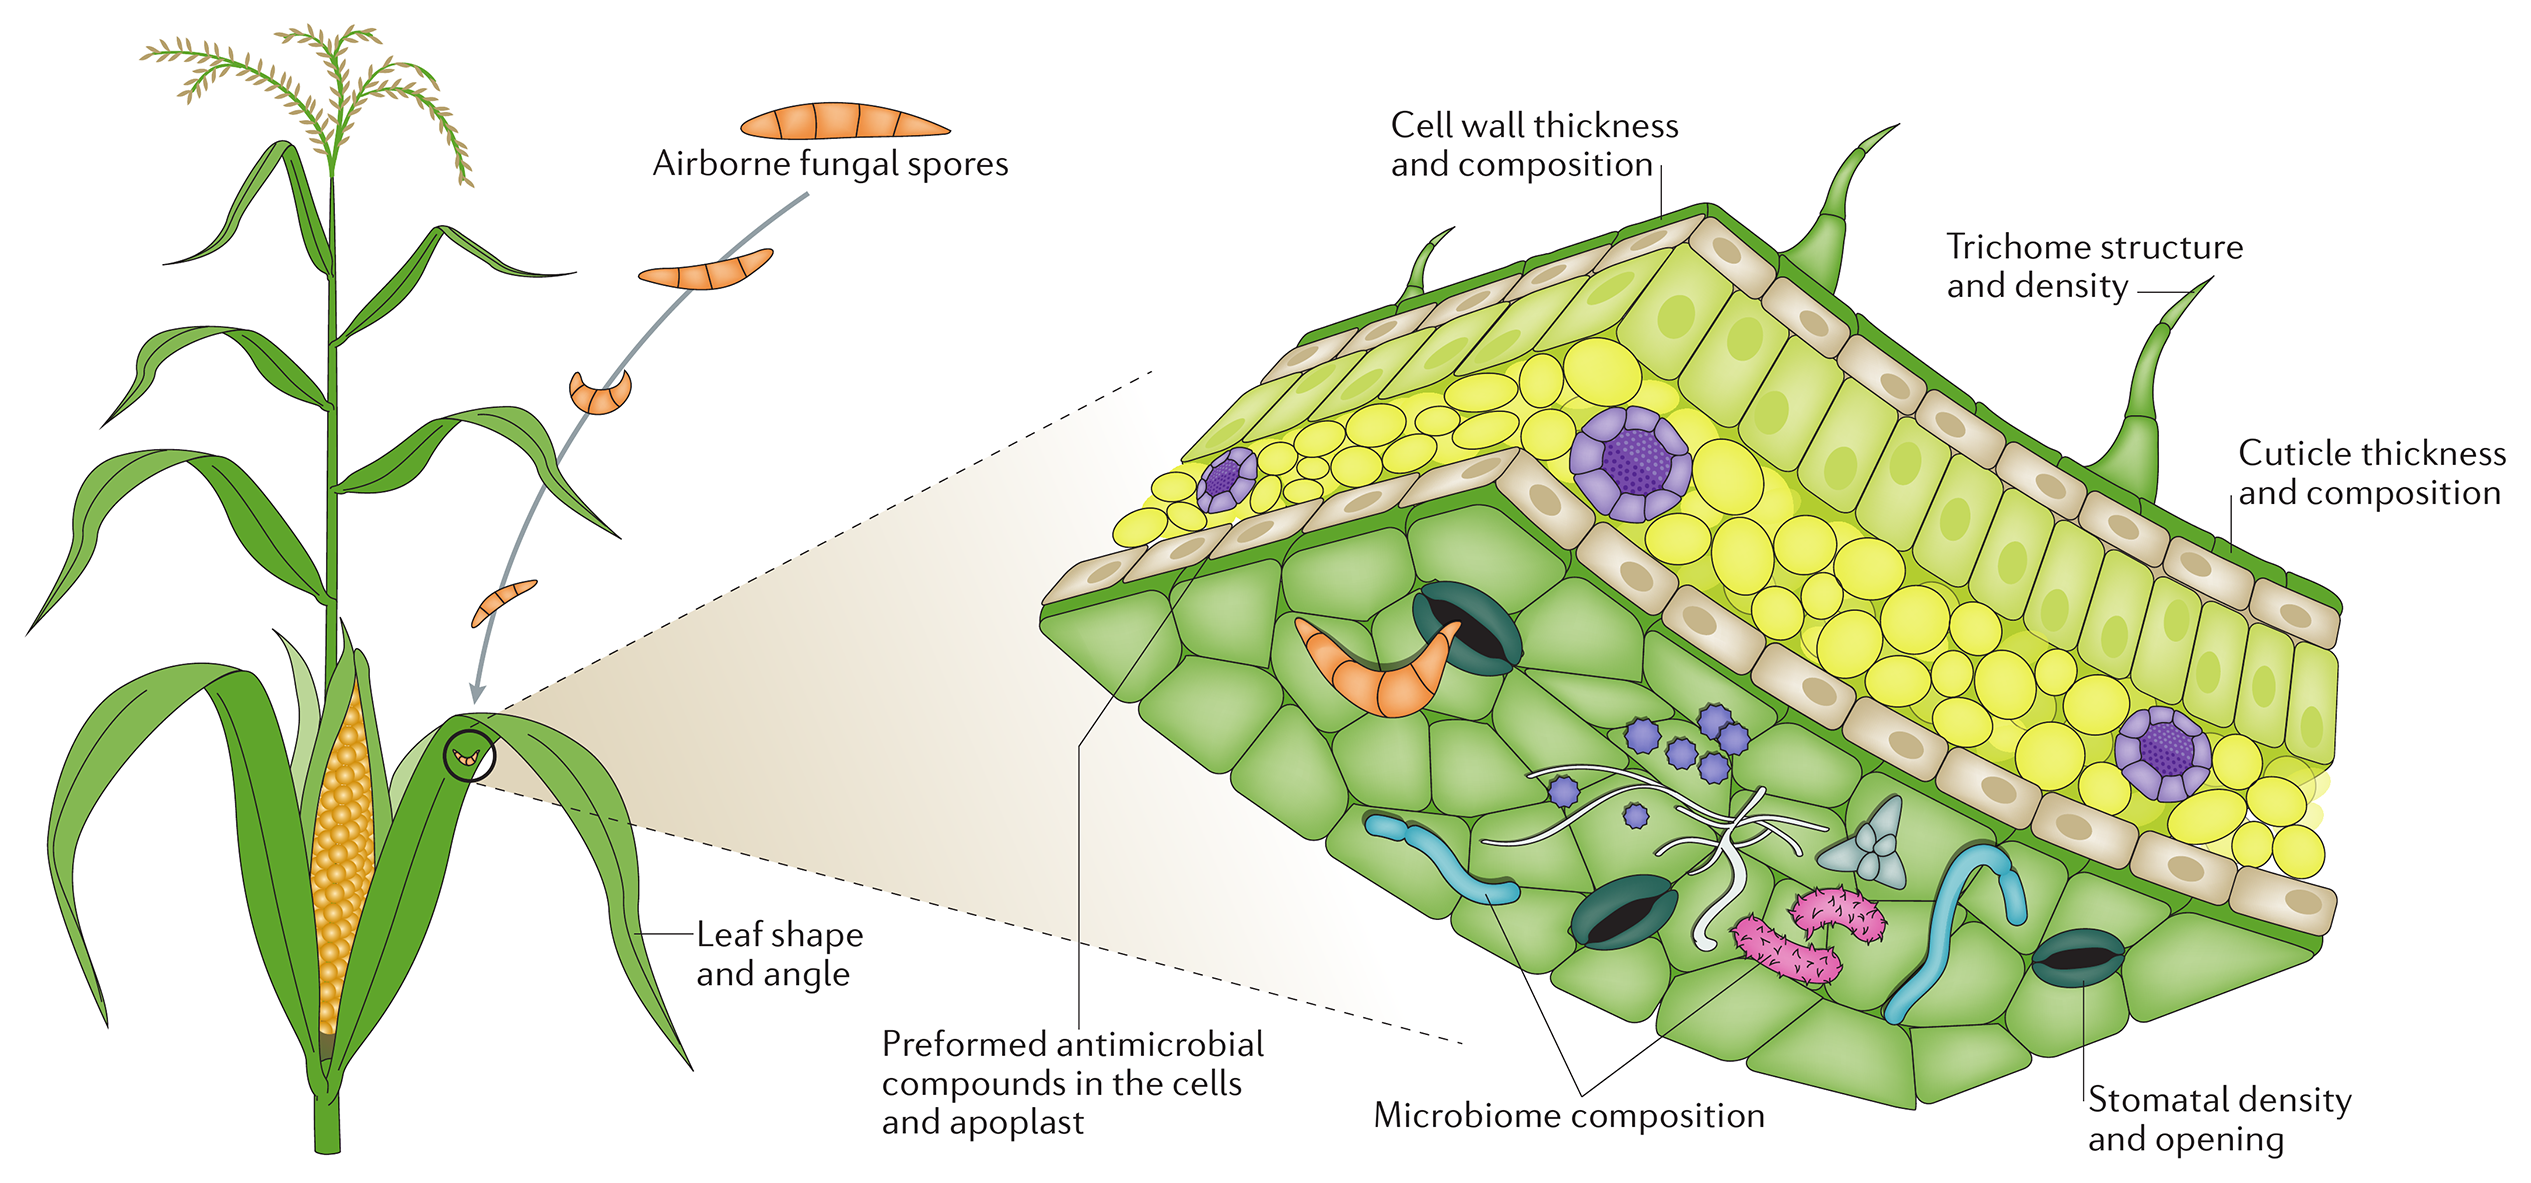
\includegraphics[width=0.8\linewidth]{../images/infection_process_plants_extracellular} \caption{Resistance mechanisms at the tissue level. At the organismal and tissue levels, the success of a pathogen can be influenced by a range of features of the morphology, biochemistry and microbiome of the plant.}\label{fig:infection-mechanism-extracellular}
\end{figure}
\end{frame}

\begin{frame}{}
\protect\hypertarget{section-19}{}
\begin{figure}
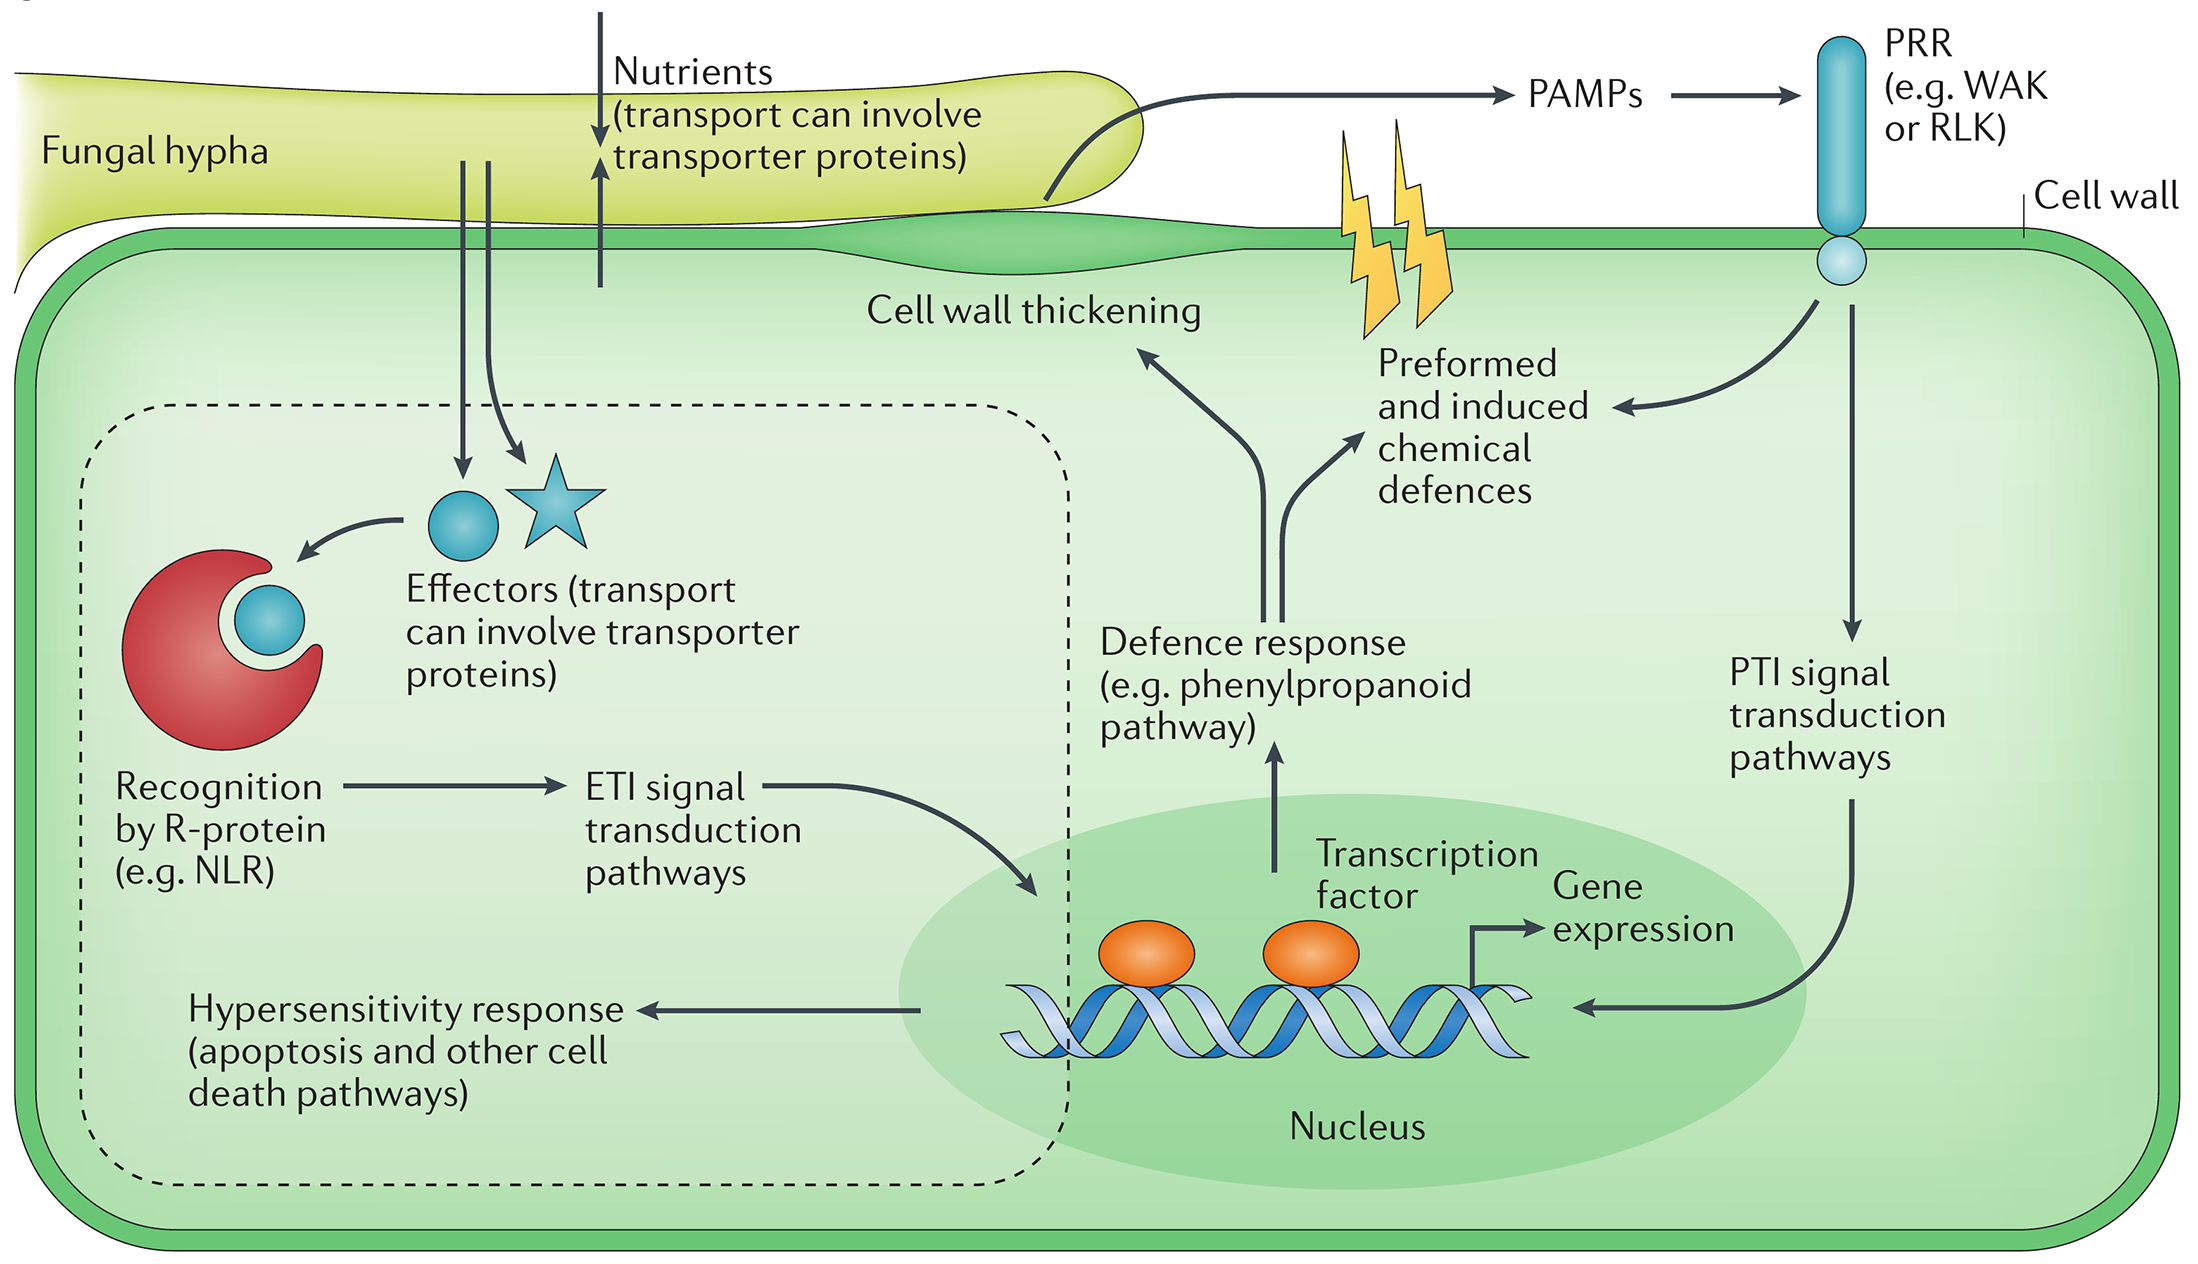
\includegraphics[width=0.78\linewidth]{../images/infection_process_plants_intracellular} \caption{At cellular level, factors that affect the ability of a pathogen to infect its plant host include defence responses triggered by recognition events in the host via PRRs, such as WAKs or RLKs, and resistance proteins (R-proteins), such as NLR proteins, nutrient availability in the apoplast and cytoplasm; pre-existing chemical factors; and cell wall constitution. These factors are affected by host genotype and are potential causes of quantitative variation. Qualitative variation in resistance usually, though not always, occurs at the level of resistance gene-effector interactions.}\label{fig:infection-mechanism-intracellular}
\end{figure}
\end{frame}

\hypertarget{genome-comparisons-of-plant-pathogens-filamentous}{%
\section{Genome comparisons of plant pathogens
(filamentous)}\label{genome-comparisons-of-plant-pathogens-filamentous}}

\begin{frame}{}
\protect\hypertarget{section-20}{}
\begin{figure}
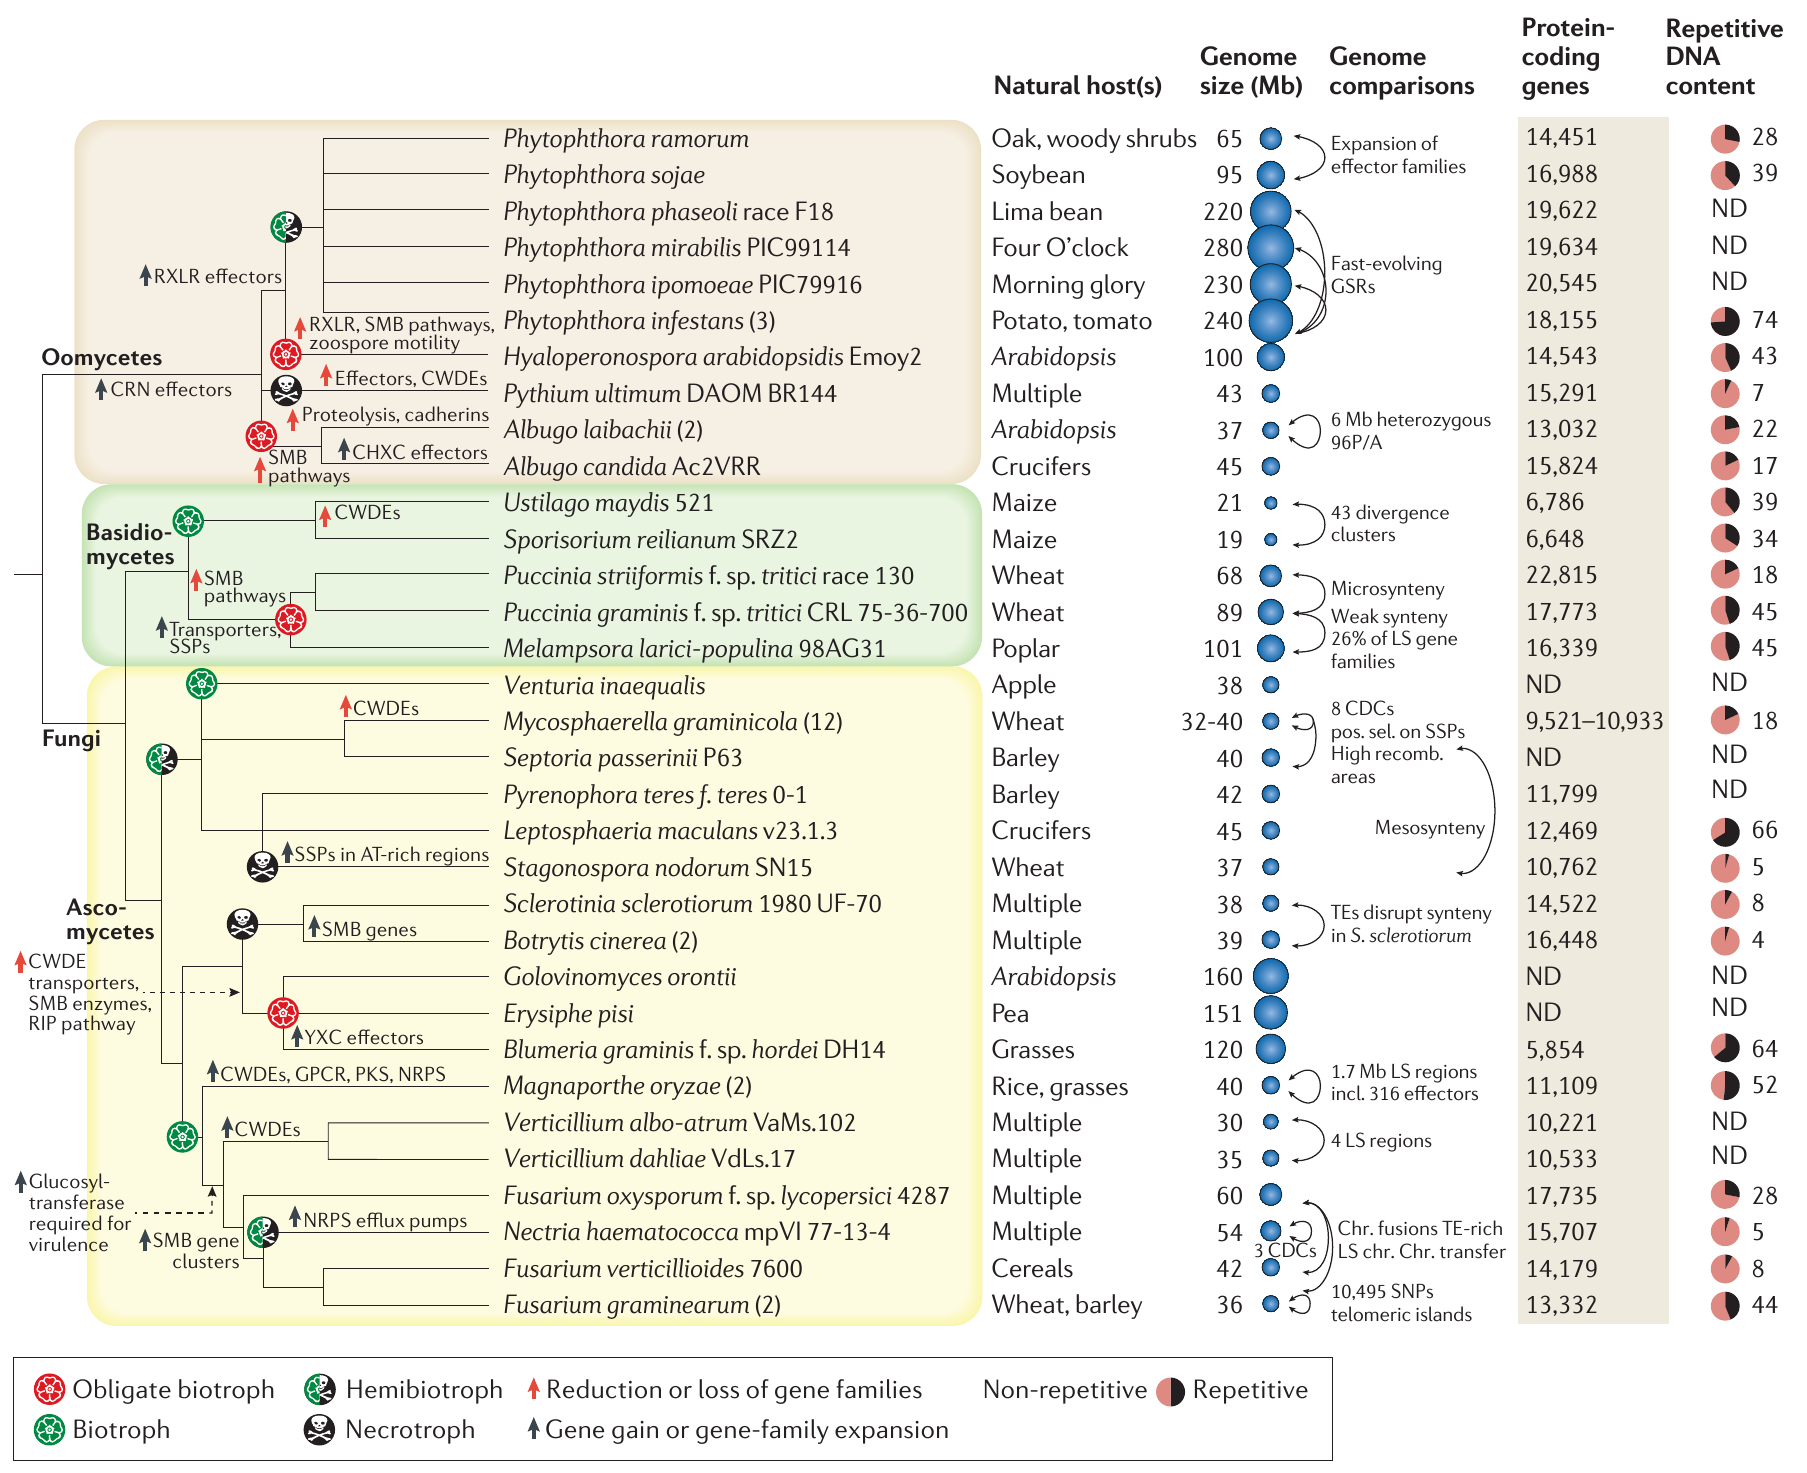
\includegraphics[width=0.4\linewidth]{../images/genome_comparison_pathogenic_fungi} \caption{Main features of sequenced filamentous plant pathogen genomes. Filamentous eukaryotic plant pathogens belong to either the fungi or the stramenopiles (oomycetes). The representative phylogeny depicts filamentous plant pathogens with sequenced genomes and has been generated using iTOL with NCBI taxonomy identifiers (branch lengths are arbitrary). Isolate identifier, or the number of isolates sequenced, is indicated next to the species name. Pathogen lifestyles and major variations in gene families are indicated along the tree branches. The principal host plants, genome size, main insights gained from genome comparisons, number of predicted protein-coding genes and repetitive DNA content (as a percentage of genome size) are shown next to the tree branches. CDC, conditionally dispensible chromosome; chr., chromosome; CNV, copy number variation; CRN, Crinkler; CWDE, cell wall-degrading enzyme; GPCR, G protein coupled receptor; GSR, gene-sparse region; incl., including; LS, lineage-specific; ND, not determined; NRPS, non-ribosomal peptide synthetase; P/A, presence/absence; PKS, polyketide synthase; pos. sel., positive selection; rec., recombination; RIP, repeat-induced point; SMB, secondary metabolite biosynthesis; SNPs, single-nucleotide polymorphisms; SSP, small secreted protein; TE, transposable element}\label{fig:pathogenic-fungi-genome-compare}
\end{figure}
\end{frame}

\hypertarget{insects}{%
\section{Insects}\label{insects}}

\begin{frame}{Major insects of Rice}
\protect\hypertarget{major-insects-of-rice}{}
\renewcommand{\arraystretch}{0.6}

\begin{table}

\caption{\label{tab:insects-damage}Major insects of rice and nature of their damange}
\centering
\fontsize{5}{7}\selectfont
\begin{tabular}[t]{>{\raggedright\arraybackslash}p{8em}>{\raggedright\arraybackslash}p{14em}>{\raggedright\arraybackslash}p{18em}}
\toprule
Damaged part & Insect & Scientific name\\
\midrule
 & Rice ear cutting caterpillar & \textit{Mythimna seperata}\\
\cmidrule{2-3}
 & Rice swarming caterpillar & \textit{Spodoptera mauritia}\\
\cmidrule{2-3}
 & Rice leaf folder & \textit{Cnaphalocrosis medinalis}\\
\cmidrule{2-3}
 & Rice caseworm & \textit{Nymphyla dpunctalis}\\
\cmidrule{2-3}
 & Rice grasshopper & \textit{Hyeroglyphus banian}\\
\cmidrule{2-3}
 & Rice hispa & \textit{Dickladispa armigera}\\
\cmidrule{2-3}
\multirow{-7}{8em}{\raggedright\arraybackslash Leaf} & Field cricket & \textit{Gryllus bimaculatus}\\
\cmidrule{1-3}
 & Yellow stem borer & \textit{Scripophaga incertulus}\\
\cmidrule{2-3}
 & Rice pink borer & \textit{Sesamia inferens}\\
\cmidrule{2-3}
 & Gall midge & \textit{Orselolia oryzae}\\
\cmidrule{2-3}
\multirow{-4}{8em}{\raggedright\arraybackslash Stem} & Striped stem borer & \textit{Chilo partellus}\\
\cmidrule{1-3}
 & Brown plant hopper & \textit{Nilaparvata lugens}\\
\cmidrule{2-3}
 & Rice thrips & \textit{Stenochaetothrips biformis}\\
\cmidrule{2-3}
\multirow{-3}{8em}{\raggedright\arraybackslash Tender shoots} & Green leaf hopper & \textit{Nephotettix virisens}\\
\cmidrule{1-3}
Root & Mole cricket & \textit{Gryllotalpa africana}\\
\cmidrule{1-3}
 & Rice earhead bug & \textit{Leptocorisa oratorious}\\
\cmidrule{2-3}
\multirow{-2}{8em}{\raggedright\arraybackslash Grain, flower} & Flower/pollen beetle & \textit{Chiloloba acuta}\\
\bottomrule
\end{tabular}
\end{table}
\end{frame}

\begin{frame}{Major Insects of Fruits and Vegetables}
\protect\hypertarget{major-insects-of-fruits-and-vegetables}{}
\renewcommand{\arraystretch}{0.6} 
\begin{table}

\caption{\label{tab:major-insects-fruits-vegetables}Insect pests of fruits and vegetables}
\centering
\fontsize{4}{6}\selectfont
\begin{tabular}[t]{>{\raggedright\arraybackslash}p{6em}>{\raggedright\arraybackslash}p{10em}>{\raggedright\arraybackslash}p{14em}>{\raggedright\arraybackslash}p{12em}>{\raggedright\arraybackslash}p{8em}>{\raggedright\arraybackslash}p{10em}}
\toprule
Crop group & Common name & Scientific name & Family & Control & Remark\\
\midrule
 & Wolly aphid & Eriosoma langierum & Hemiptera &  & \\
\cmidrule{2-6}
 & San jose scale & Quadraspidiotus perniciosus & Hemiptera &  & \\
\cmidrule{2-6}
 & Stem borer & Apriona cinera & Coleoptera &  & \\
\cmidrule{2-6}
 & Root borer & Dorysthenes hugeli & Coleoptera &  & \\
\cmidrule{2-6}
\multirow{-5}{6em}{\raggedright\arraybackslash Apple} & Codling moth & Cydia pomonella & Lepidoptera &  & \\
\cmidrule{1-6}
 & Rhizome weevil & Cosmopolites sordidus & Coleoptera &  & \\
\cmidrule{2-6}
 & Pseudostem weevil & Odoiporus longicollis & Coleoptera &  & \\
\cmidrule{2-6}
 & Skipper & Erionata thrax thrax & Lepidoptera &  & \\
\cmidrule{2-6}
 & Leaf and fruit scarring beetle & Nodostoma viridipennis & Coleoptera &  & \\
\cmidrule{2-6}
 & Aphid & Pentalonia nigronervosa & Hemiptera &  & \\
\cmidrule{2-6}
 & Lace-wing bug & Stephanitis typica & Hemiptera &  & \\
\cmidrule{2-6}
\multirow{-7}{6em}{\raggedright\arraybackslash Banana} & Fruit fly & Bactrocera musae & Hemiptera (Tephritidae) &  & \\
\cmidrule{1-6}
 & Tent caterpillar & Malacosoma indicum & Lepidoptera &  & Also affects apricot and walnut\\
\cmidrule{2-6}
\multirow{-2}{6em}{\raggedright\arraybackslash Peach} & Leaf curl aphid & Brachycaudia helichrysi & Hemiptera &  & \\
\bottomrule
\end{tabular}
\end{table}
\end{frame}

\begin{frame}{}
\protect\hypertarget{section-21}{}
\begin{table}

\caption{\label{tab:unnamed-chunk-3}Insect pests of fruits and vegetables (...continued)}
\centering
\fontsize{4}{6}\selectfont
\begin{tabular}[t]{>{\raggedright\arraybackslash}p{5em}>{\raggedright\arraybackslash}p{13em}>{\raggedright\arraybackslash}p{14em}>{\raggedright\arraybackslash}p{14em}>{\raggedright\arraybackslash}p{7em}>{\raggedright\arraybackslash}p{12em}}
\toprule
Crop group & Common name & Scientific name & Family & Control & Remark\\
\midrule
 & Citrus psylla & Diaphorina citri & Hemiptera &  & \\
\cmidrule{2-6}
 & Oriental fruit fly & Bactocera dorsalis & Diptera (Tephritidae) &  & \\
\cmidrule{2-6}
 & Stink bug & Rhynchocoris poseidon & Hemiptera &  & \\
\cmidrule{2-6}
 & Red scale & Aonideiella aurantii & Hemiptera &  & \\
\cmidrule{2-6}
 & Citrus aphid & Toxoptera citricidus & Hemiptera &  & \\
\cmidrule{2-6}
 & Orange stem borer & Stomatimum barbatum & Coleoptera &  & \\
\cmidrule{2-6}
\multirow{-7}{5em}{\raggedright\arraybackslash Citrus} & Citrus mealy bug & Planococcus citri & Hemiptera &  & \\
\cmidrule{1-6}
 & Hopper & Idioscopus nitidulus & Hemiptera (Cicadellidae) &  & \\
\cmidrule{2-6}
 & Fruit fly & Bactrocera dorsalis & Hemiptera (Tephritidae) &  & \\
\cmidrule{2-6}
 & Mealy bug & Drosicha mangiferae & Hemiptera &  & \\
\cmidrule{2-6}
 & Stem borer & Bactrocera rufomaculata & Coleoptera &  & \\
\cmidrule{2-6}
 & Leaf webber & Orthaga spp. & Lepidoptera &  & \\
\cmidrule{2-6}
 & Stone weevil & Sternochetus mangiferae & Coleoptera &  & \\
\cmidrule{2-6}
 & Gall psyllid & Apsylla cistella & Hemiptera &  & \\
\cmidrule{2-6}
\multirow{-8}{5em}{\raggedright\arraybackslash Mango} & Slug caterpillar, Mango leaf cutting weevil &  &  &  & \\
\bottomrule
\end{tabular}
\end{table}
\end{frame}

\begin{frame}{}
\protect\hypertarget{section-22}{}
\begin{table}

\caption{\label{tab:unnamed-chunk-4}Insect pests of fruits and vegetables (...continued)}
\centering
\fontsize{5}{7}\selectfont
\begin{tabular}[t]{>{\raggedright\arraybackslash}p{6em}>{\raggedright\arraybackslash}p{12em}>{\raggedright\arraybackslash}p{14em}>{\raggedright\arraybackslash}p{14em}>{\raggedright\arraybackslash}p{8em}>{\raggedright\arraybackslash}p{8em}}
\toprule
Crop group & Common name & Scientific name & Family & Control & Remark\\
\midrule
 & Rice weevil & Sitophus oryzae & Coleoptera (Curculionidae) &  & \\
\cmidrule{2-6}
 & Maize weevil & Sitophus zeamais & Coleoptera (Curculionidae) &  & \\
\cmidrule{2-6}
 & Angoumois grain moth & Sitotroga cerealella & Lepidoptera (Gelechiidae) &  & \\
\cmidrule{2-6}
 & Lesser grain borer & Rhizopertha dominica & Coleoptera (Bostrichidae) &  & \\
\cmidrule{2-6}
 & Rice moth & Corcyra cephalonica & Lepidoptera (Pyralidae) &  & \\
\cmidrule{2-6}
 & Khapra beetle & Trogoderma granarium & Coleoptera (Dermastidae) &  & \\
\cmidrule{2-6}
 & Pulse beetle & Callosobruchus chinensis & Coleoptera (Bruchidae) &  & \\
\cmidrule{2-6}
 & Cowpea beetle & Callosobruchus maculates & Coleoptera (Bruchidae) &  & \\
\cmidrule{2-6}
 & Rust red flour beetle & Tribolium castaneum & Coleoptera (Tenebrionidae) &  & \\
\cmidrule{2-6}
 & Confused flour beetle & Tribolium confusum & Coleoptera (Tenebrionidae) &  & \\
\cmidrule{2-6}
 & Warehouse moth & Ephestia cautella & Lepidoptera (Pyralidae) &  & \\
\cmidrule{2-6}
 & Indian meal moth & Plodia interpunctella & Lepidoptera (Phycitidae) &  & \\
\cmidrule{2-6}
 & Bean weevil & Acanthoscelides obtectus & Coleoptera (Bruchidae) &  & \\
\cmidrule{2-6}
\multirow{-14}{6em}{\raggedright\arraybackslash Storage pests} & Granary weevil & Sitophilus granaries & Coleoptera (Curculionidae) &  & \\
\bottomrule
\end{tabular}
\end{table}
\end{frame}

\begin{frame}{}
\protect\hypertarget{section-23}{}
\begin{table}

\caption{\label{tab:unnamed-chunk-5}Insect pests of fruits and vegetables (...continued)}
\centering
\fontsize{4}{6}\selectfont
\begin{tabular}[t]{>{\raggedright\arraybackslash}p{6em}>{\raggedright\arraybackslash}p{12em}>{\raggedright\arraybackslash}p{15em}>{\raggedright\arraybackslash}p{14em}>{\raggedright\arraybackslash}p{6em}>{\raggedright\arraybackslash}p{16em}}
\toprule
Crop group & Common name & Scientific name & Family & Control & Remark\\
\midrule
 & Shoot and fruit borer & Leucinodes orbonalis & Lepidoptera &  & \\
\cmidrule{2-6}
 & Leaf folder & Eublemma olivacea & Lepidoptera &  & \\
\cmidrule{2-6}
 & Leaf webber & Herpetogramma bipuncatalis & Lepidoptera &  & \\
\cmidrule{2-6}
 & Spotted beetle & Epilachna vigintioctopunctata & Coleoptera &  & \\
\cmidrule{2-6}
\multirow{-5}{6em}{\raggedright\arraybackslash Brinjal} & Aphid, Cotton jassid, Tobaccoo caterpillar, Soybean hairy caterpillar, White fly, Green semilooper, Grasshopper, Red ant, White grub &  &  &  & Minor insects\\
\cmidrule{1-6}
 & Potato tuber moth & Phthorimaea operculella & Lepidoptera &  & \\
\cmidrule{2-6}
 & Red ant & Dorylus orientalis & Hymenoptera &  & \\
\cmidrule{2-6}
\multirow{-3}{6em}{\raggedright\arraybackslash Potato} & Silver white fly & Bemisia tabaci & Homoptera &  & Variants of white flies of economic importance are: Aleurocanthus woglumi (citrus blackfly), which, in spite of its color, is a whitefly that attacks citrus. Aleyrodes proletella (cabbage whitefly), is a pest of various Brassica crops. Trialeurodes vaporariorum (greenhouse whitefly), a major pest of greenhouse fruit, vegetables, and ornamentals.\\
\bottomrule
\end{tabular}
\end{table}
\end{frame}

\begin{frame}{}
\protect\hypertarget{section-24}{}
\begin{table}

\caption{\label{tab:unnamed-chunk-6}Insect pests of fruits and vegetables (...continued)}
\centering
\fontsize{4}{6}\selectfont
\begin{tabular}[t]{>{\raggedright\arraybackslash}p{5em}>{\raggedright\arraybackslash}p{10em}>{\raggedright\arraybackslash}p{15em}>{\raggedright\arraybackslash}p{12em}>{\raggedright\arraybackslash}p{6em}>{\raggedright\arraybackslash}p{22em}}
\toprule
Crop group & Common name & Scientific name & Family & Control & Remark\\
\midrule
 & American bollworm/Fruit borer & Helicoverpa armigera & Noctuidae &  & Bolls how regular, circular bore holes; A single larvae can damage 30-40 bolls; Inundative release of egg parasitoid, Trichogramma spp., at 6.25 cc/ha at 15 days interval, 3 times from 45 DAS; Releasing of predator Chrysoperla carnea 100000/ha at 6th, 13th and 14th week after sowing; During bolling and maturation apply one of the following (1000 liter per hectare spray): Quinalphos 25EC 2.0 liter per hectare, Carbaryl 50 WP 2.5 kg per hectare, Cypermethrin 10 EC 600-800 ml per hectare.\\
\cmidrule{2-6}
 & Pink bollworm & Pectinophora gossypiella & Lepidoptera (Gelechiidae) &  & \\
\cmidrule{2-6}
 & Spotted bollworm & Earias vittella & Lepidoptera (Noctuidae) &  & \\
\cmidrule{2-6}
 & Tobaccoo cutworm & Spodoptera litura & Lepidoptera (Noctuidae) &  & \\
\cmidrule{2-6}
 & Cotton aphid & Aphis gossypii & Hemiptera (Aphididae) &  & \\
\cmidrule{2-6}
 & Thrips & Thrips tabaci & Thysanoptera &  & \\
\cmidrule{2-6}
 & White fly & Bemisia tabaci & Hemiptera (Aleyrodidae) &  & \\
\cmidrule{2-6}
\multirow{-8}{5em}{\raggedright\arraybackslash Cotton} & Red cotton bug & Dysdercus cingulatus & Hemiptera (Pyrrhocoridae) &  & \\
\bottomrule
\end{tabular}
\end{table}
\end{frame}

\begin{frame}{}
\protect\hypertarget{section-25}{}
\begin{table}

\caption{\label{tab:unnamed-chunk-7}Insect pests of fruits and vegetables (...continued)}
\centering
\fontsize{4}{6}\selectfont
\begin{tabular}[t]{>{\raggedright\arraybackslash}p{6em}>{\raggedright\arraybackslash}p{12em}>{\raggedright\arraybackslash}p{14em}>{\raggedright\arraybackslash}p{14em}>{\raggedright\arraybackslash}p{14em}>{\raggedright\arraybackslash}p{8em}}
\toprule
Crop group & Common name & Scientific name & Family & Control & Remark\\
\midrule
 & Cabbage butterfly & Pieris brassicae & Lepidoptera & Dichlorovos 76 EC, Nuvan 1 ml, Malation 50\% EC 2ml & \\
\cmidrule{2-6}
 & Diamond-back moth & Plutella xylostella & Lepidoptera & DBM lure, Azadirachtin 0.003\% EC, Beauveria bassiana, Emamectin benzoate, Cypermethrin 10\% EC 2ml & \\
\cmidrule{2-6}
 & Tobaccoo caterpillar & Spodoptera litura & Lepidoptera & Spodo-lure & \\
\cmidrule{2-6}
 & Mustard aphid & Lipaphis erysimi & Homoptera & Augmentation of natural predators Lady bird beetle (Coccinella septumpunctata) and Syrphid fly; Malathion 50 EC 1.5-2 ml per liter of water & \\
\cmidrule{2-6}
 & Mustard sawfly & Athalia lugens & Hymenoptera & Summer ploughing & \\
\cmidrule{2-6}
 & Cutworm & Agrotis ipsilon, A. segetum & Lepidoptera &  & \\
\cmidrule{2-6}
 & Flea beetle & Phyllotreta cruciferae & Coleoptera &  & \\
\cmidrule{2-6}
\multirow{-8}{6em}{\raggedright\arraybackslash Cruciferous vegetables} & Semi looper & Thysanoplusia orichalcea & Lepidoptera &  & \\
\bottomrule
\end{tabular}
\end{table}
\end{frame}

\begin{frame}{}
\protect\hypertarget{section-26}{}
\begin{table}

\caption{\label{tab:unnamed-chunk-8}Insect pests of fruits and vegetables (...continued)}
\centering
\fontsize{4}{6}\selectfont
\begin{tabular}[t]{>{\raggedright\arraybackslash}p{6em}>{\raggedright\arraybackslash}p{12em}>{\raggedright\arraybackslash}p{14em}>{\raggedright\arraybackslash}p{14em}>{\raggedright\arraybackslash}p{14em}>{\raggedright\arraybackslash}p{8em}}
\toprule
Crop group & Common name & Scientific name & Family & Control & Remark\\
\midrule
 & Re pumpkin beetle & Aulacophora foevicolis & Coleoptera &  & \\
\cmidrule{2-6}
 & Cucurbit stink bug & Cordius janus & Hemiptera &  & \\
\cmidrule{2-6}
 & Pumpkin fruit fly & Bactrocera cucurbitae & Diptera &  & \\
\cmidrule{2-6}
 & Spotted beetle & Epilachna vigintioctopunctata & Coleoptera &  & \\
\cmidrule{2-6}
\multirow{-5}{6em}{\raggedright\arraybackslash Cucurbit crops} & Cutworm, Semi-looper, Flea beetle, Aphid, White fly, Stem boring beetle, Banded blister beetle & Mylabris orientalis &  &  & Minior insects\\
\cmidrule{1-6}
 & Aphid & Aphis gossypii, Myzus persicae & Hemiptera &  & \\
\cmidrule{2-6}
 & Pea leaf miner & Liriomyza huidobrensis & Agromyzidae &  & \\
\cmidrule{2-6}
\multirow{-3}{6em}{\raggedright\arraybackslash Solanaceous crops} & Cutworm, Spotted beetle, White grub, Wireworm, Tobaccoo caterpillar, Flea beetle, Soybean, Hairy caterpillar &  &  &  & Minor insects\\
\bottomrule
\end{tabular}
\end{table}
\end{frame}

\begin{frame}{}
\protect\hypertarget{section-27}{}
\begin{table}

\caption{\label{tab:unnamed-chunk-9}Insect pests of fruits and vegetables (...continued)}
\centering
\fontsize{5}{7}\selectfont
\begin{tabular}[t]{>{\raggedright\arraybackslash}p{6em}>{\raggedright\arraybackslash}p{10em}>{\raggedright\arraybackslash}p{14em}>{\raggedright\arraybackslash}p{12em}>{\raggedright\arraybackslash}p{8em}>{\raggedright\arraybackslash}p{8em}}
\toprule
Crop group & Common name & Scientific name & Family & Control & Remark\\
\midrule
 & Tomato fruit borer & Helicoverpa armigera & Lepidoptera &  & \\
\cmidrule{2-6}
 & Jassid & Amarasca biguttula & Hemiptera &  & \\
\cmidrule{2-6}
\multirow{-3}{6em}{\raggedright\arraybackslash Tomato} & Tomato leaf miner & Tuta absoluta & Lepidoptera &  & \\
\cmidrule{1-6}
 & White stem borer & Xylotrechus quadripes & Coleoptera &  & \\
\cmidrule{2-6}
 & Berry borer & Hypothenemus hampei & Coleoptera &  & \\
\cmidrule{2-6}
 & Shoot-hole borer & Xylosandrus compactus & Coleoptera &  & \\
\cmidrule{2-6}
 & Stripped mealy bug & Ferrisia virgata & Hemiptera &  & \\
\cmidrule{2-6}
 & Helmet scale & Saissetia coffeae & Hemiptera &  & \\
\cmidrule{2-6}
\multirow{-6}{6em}{\raggedright\arraybackslash Coffee} & Gren bug & Coccus viridis & Hemiptera &  & \\
\cmidrule{1-6}
 & Mosquito/Plant bug & Belopeltis theivora & Hemiptera &  & \\
\cmidrule{2-6}
 & Red spider mite & Oligonychus coffeae & Acarina &  & \\
\cmidrule{2-6}
 & Scarlet mite & Brevipalpus phoenicis & Acarina &  & \\
\cmidrule{2-6}
\multirow{-4}{6em}{\raggedright\arraybackslash Tea} & Purple mite & Calacarus carinatus & Acarina &  & \\
\bottomrule
\end{tabular}
\end{table}
\end{frame}

\hypertarget{bibliography}{%
\section{Bibliography}\label{bibliography}}

\begin{frame}{References}
\protect\hypertarget{references}{}
\end{frame}

          \begin{frame}[allowframebreaks]{}
    \bibliographytrue
    \bibliography{./../bibliographies.bib}
    \end{frame}
  


\end{document}
